\chapter{Eksperimenti in rezultati}\label{sec:eksperimenti}

\section{Optimizacije in implementacije}

\subsection{Optimizacija HOOF deskriptorjev}
Parameter $N_{HOOF}$ smo določili na podlagi rezultatov evaluacije v tabeli \ref{tab:nhoof} in grafov korelacije med referenčnimi podatki in predikcijo \ref{fig:corr-hoof}. Za evaluacijo smo uporabili učne vzorce hrbtne kamere preliminarnih laboratorijskih testov. Evaluirali smo samo za podatke energijske porabe $W$. Pridobljene značilke deskriptorjev smo normirali na intervalu $[-1,1]$ in jih uporabili za učenje regresijskega modela z metodo podpornih vektorjev $\epsilon$-SVR in jedrom RBF. Metode so podrobneje predstavljene v poglavju \ref{sec:matematicni-modeli}. Za določitev optimalnih parametrov, ki so predstavljeni v tabeli \ref{tab:nhoof-param}, smo uporabili optimizacijsko metodo mrežnega iskanja \cite{hsu2003practical}. Rezultate smo filtrirali še s Kalmanovim filtrom, ki je predstavljen v \ref{sec:kalmanov-filter}.

\begin{table}[htb]
	\centering
    \begin{tabular}{S[table-format=2.0] S[table-format=2.3] S[table-format=1.3] S[table-format=1.3] S[table-format=1.3]}
    \toprule
    \thead{$\mathbf{N_{HOOF}}$} & \thead{$\mathbf{C}$} & \thead{$\mathbf{\gamma}$} & \thead{$\mathbf{\epsilon}$} & \thead{MSE} \\ 
    \midrule
    30 & 8 & 0.707 & 0.812 & 7.903 \\
    60 & 8 & 0.354 & 0.379 & 7.320 \\
    120 & 11.314 & 0.177 & 0.536 & 6.998 \\
    160 & 11.314 & 0.125 & 0.616 & 6.832 \\
    \bottomrule
    \end{tabular}
    \caption[Optimalni parameteri RBF jedra modelov za določitev $N_{HOOF}$]{Optimalni parametri RBF jedra za modele z različnim številom stolpcev $N_{HOOF}$ v HOOF deskriptorju.}
    \label{tab:nhoof-param}
\end{table}

V tabeli \ref{tab:nhoof} lahko vidimo, da se povečevanjem števila stolpcev rezultati bistveno ne razlikujejo. Najbojlši rezultate nam sicer daje $120$ stolpcev, vendar pa smo za potrebe naše metode uporabili $N_{HOOF}=60$, ki je ravno tako dal zadovoljive rezultate. S takim številom smo zagotovili dobro delovanje glede na minimalno vrednost, še vseeno pa ne gre za tako veliko število, ko bi do izraza prišle amplitude šumnih vektorjev.

\begin{table}[htb]
	\centering
    \begin{tabular}{S[table-format=2.0] S[table-format=1.3] S[table-format=1.3] S[table-format=1.3] S[table-format=2.2]}
    \toprule
    \thead{$\mathbf{N_{HOOF}}$} & \thead{$\mathbf{r}$} & \thead{RAE} & \thead{RRSE} & \thead{nSV [\%]}\\
    \midrule%nSV
    30 & 0.978 & 0.296 & 0.304 & \boldentry{2.2}{62.81}\\%18089
    \boldentry{2.0}{60} & 0.980 & 0.277 & 0.289 & 81.21\\%23388
    120 & \boldentry{1.3}{0.983} & \boldentry{1.3}{0.261} & \boldentry{1.3}{0.273} & 74.39\\%21424
    160 & 0.982 & 0.272 & 0.284 & 71.68\\%20644
    \bottomrule
    \end{tabular}
    \caption[Rezultati evaluacije modelov z različnim $N_{HOOF}$]{Rezultati evaluacije modelov z različnim številom stolpcev $N_{HOOF}$ HOOF deskriptorja. Optimalni rezultati so odebeljeni. Kljub dobrim rezultatom modela z $N_{HOOF}=120$ smo izbrali $N_{HOOF}=60$, ker nanj šum manj vpliva.}
    \label{tab:nhoof}
\end{table}

\begin{figure}[htb]
	\centering
    \begin{subfigure}[t]{0.45\columnwidth}
    	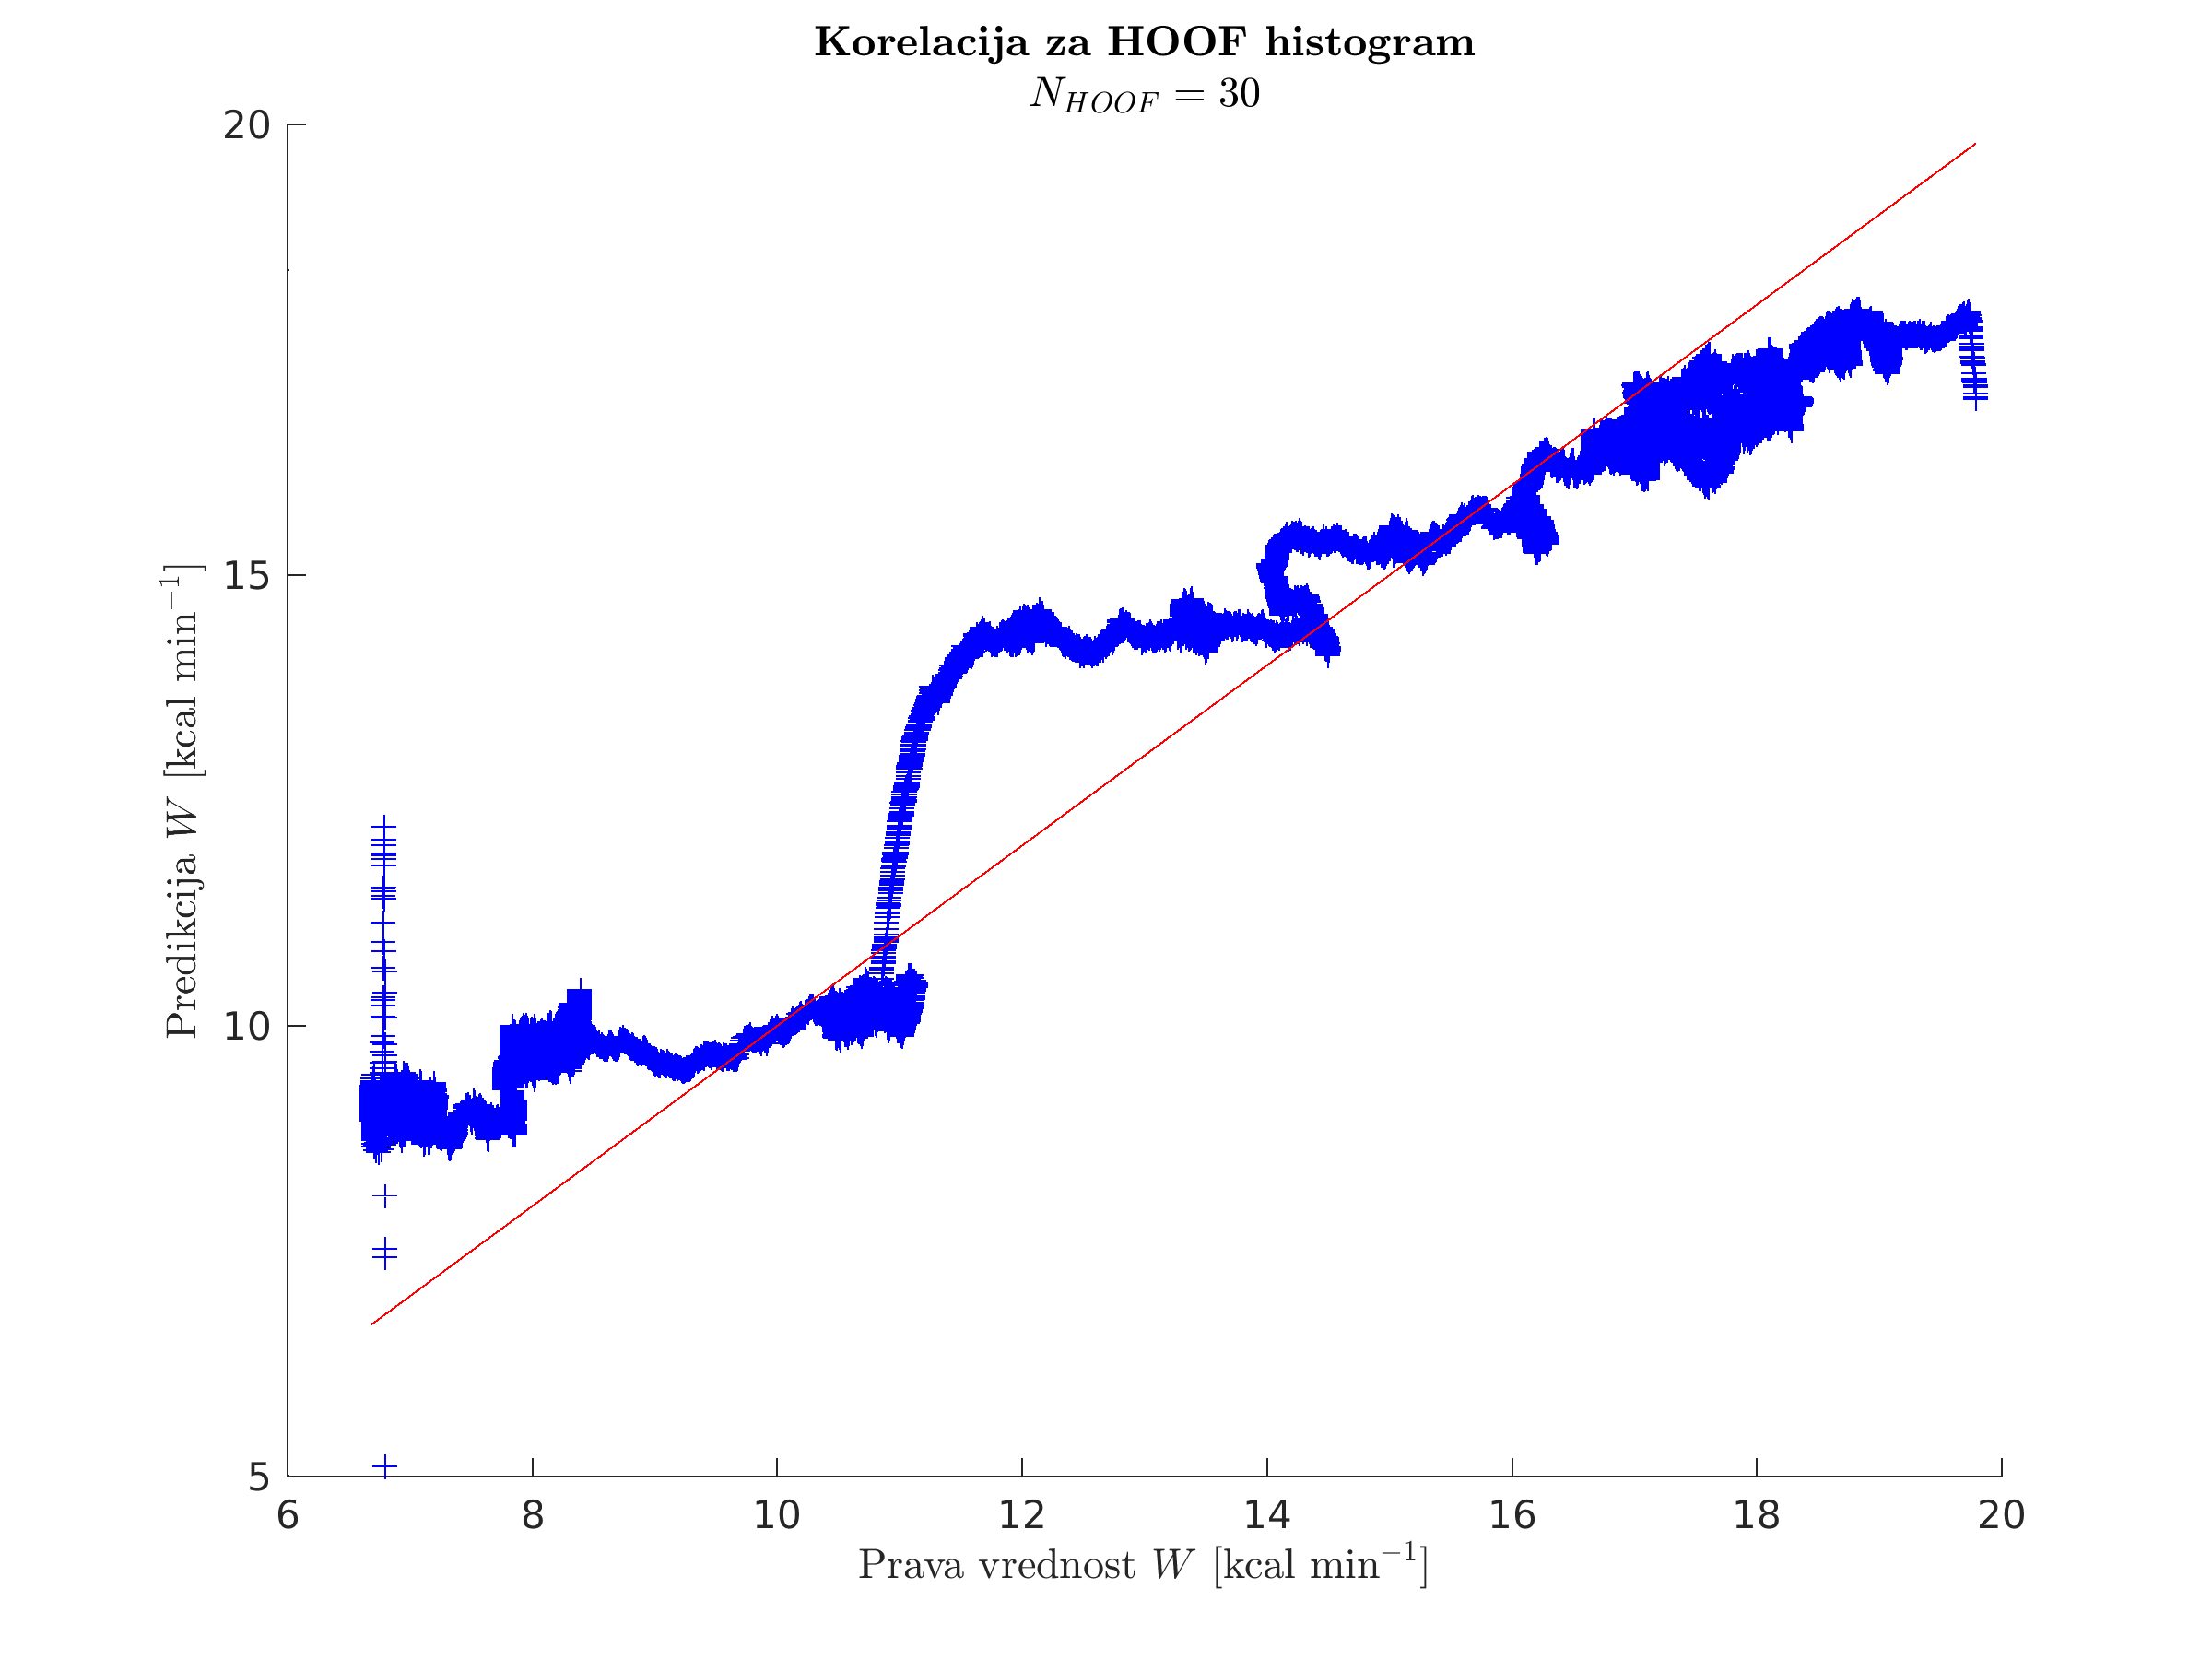
\includegraphics[width=\columnwidth]{./Slike/corr-hoof-30.png}
        \caption{Korelacija $N_{HOOF}=30$.}
        \label{fig:corr-hoof-30}
    \end{subfigure}
    ~
    \begin{subfigure}[t]{0.45\columnwidth}
      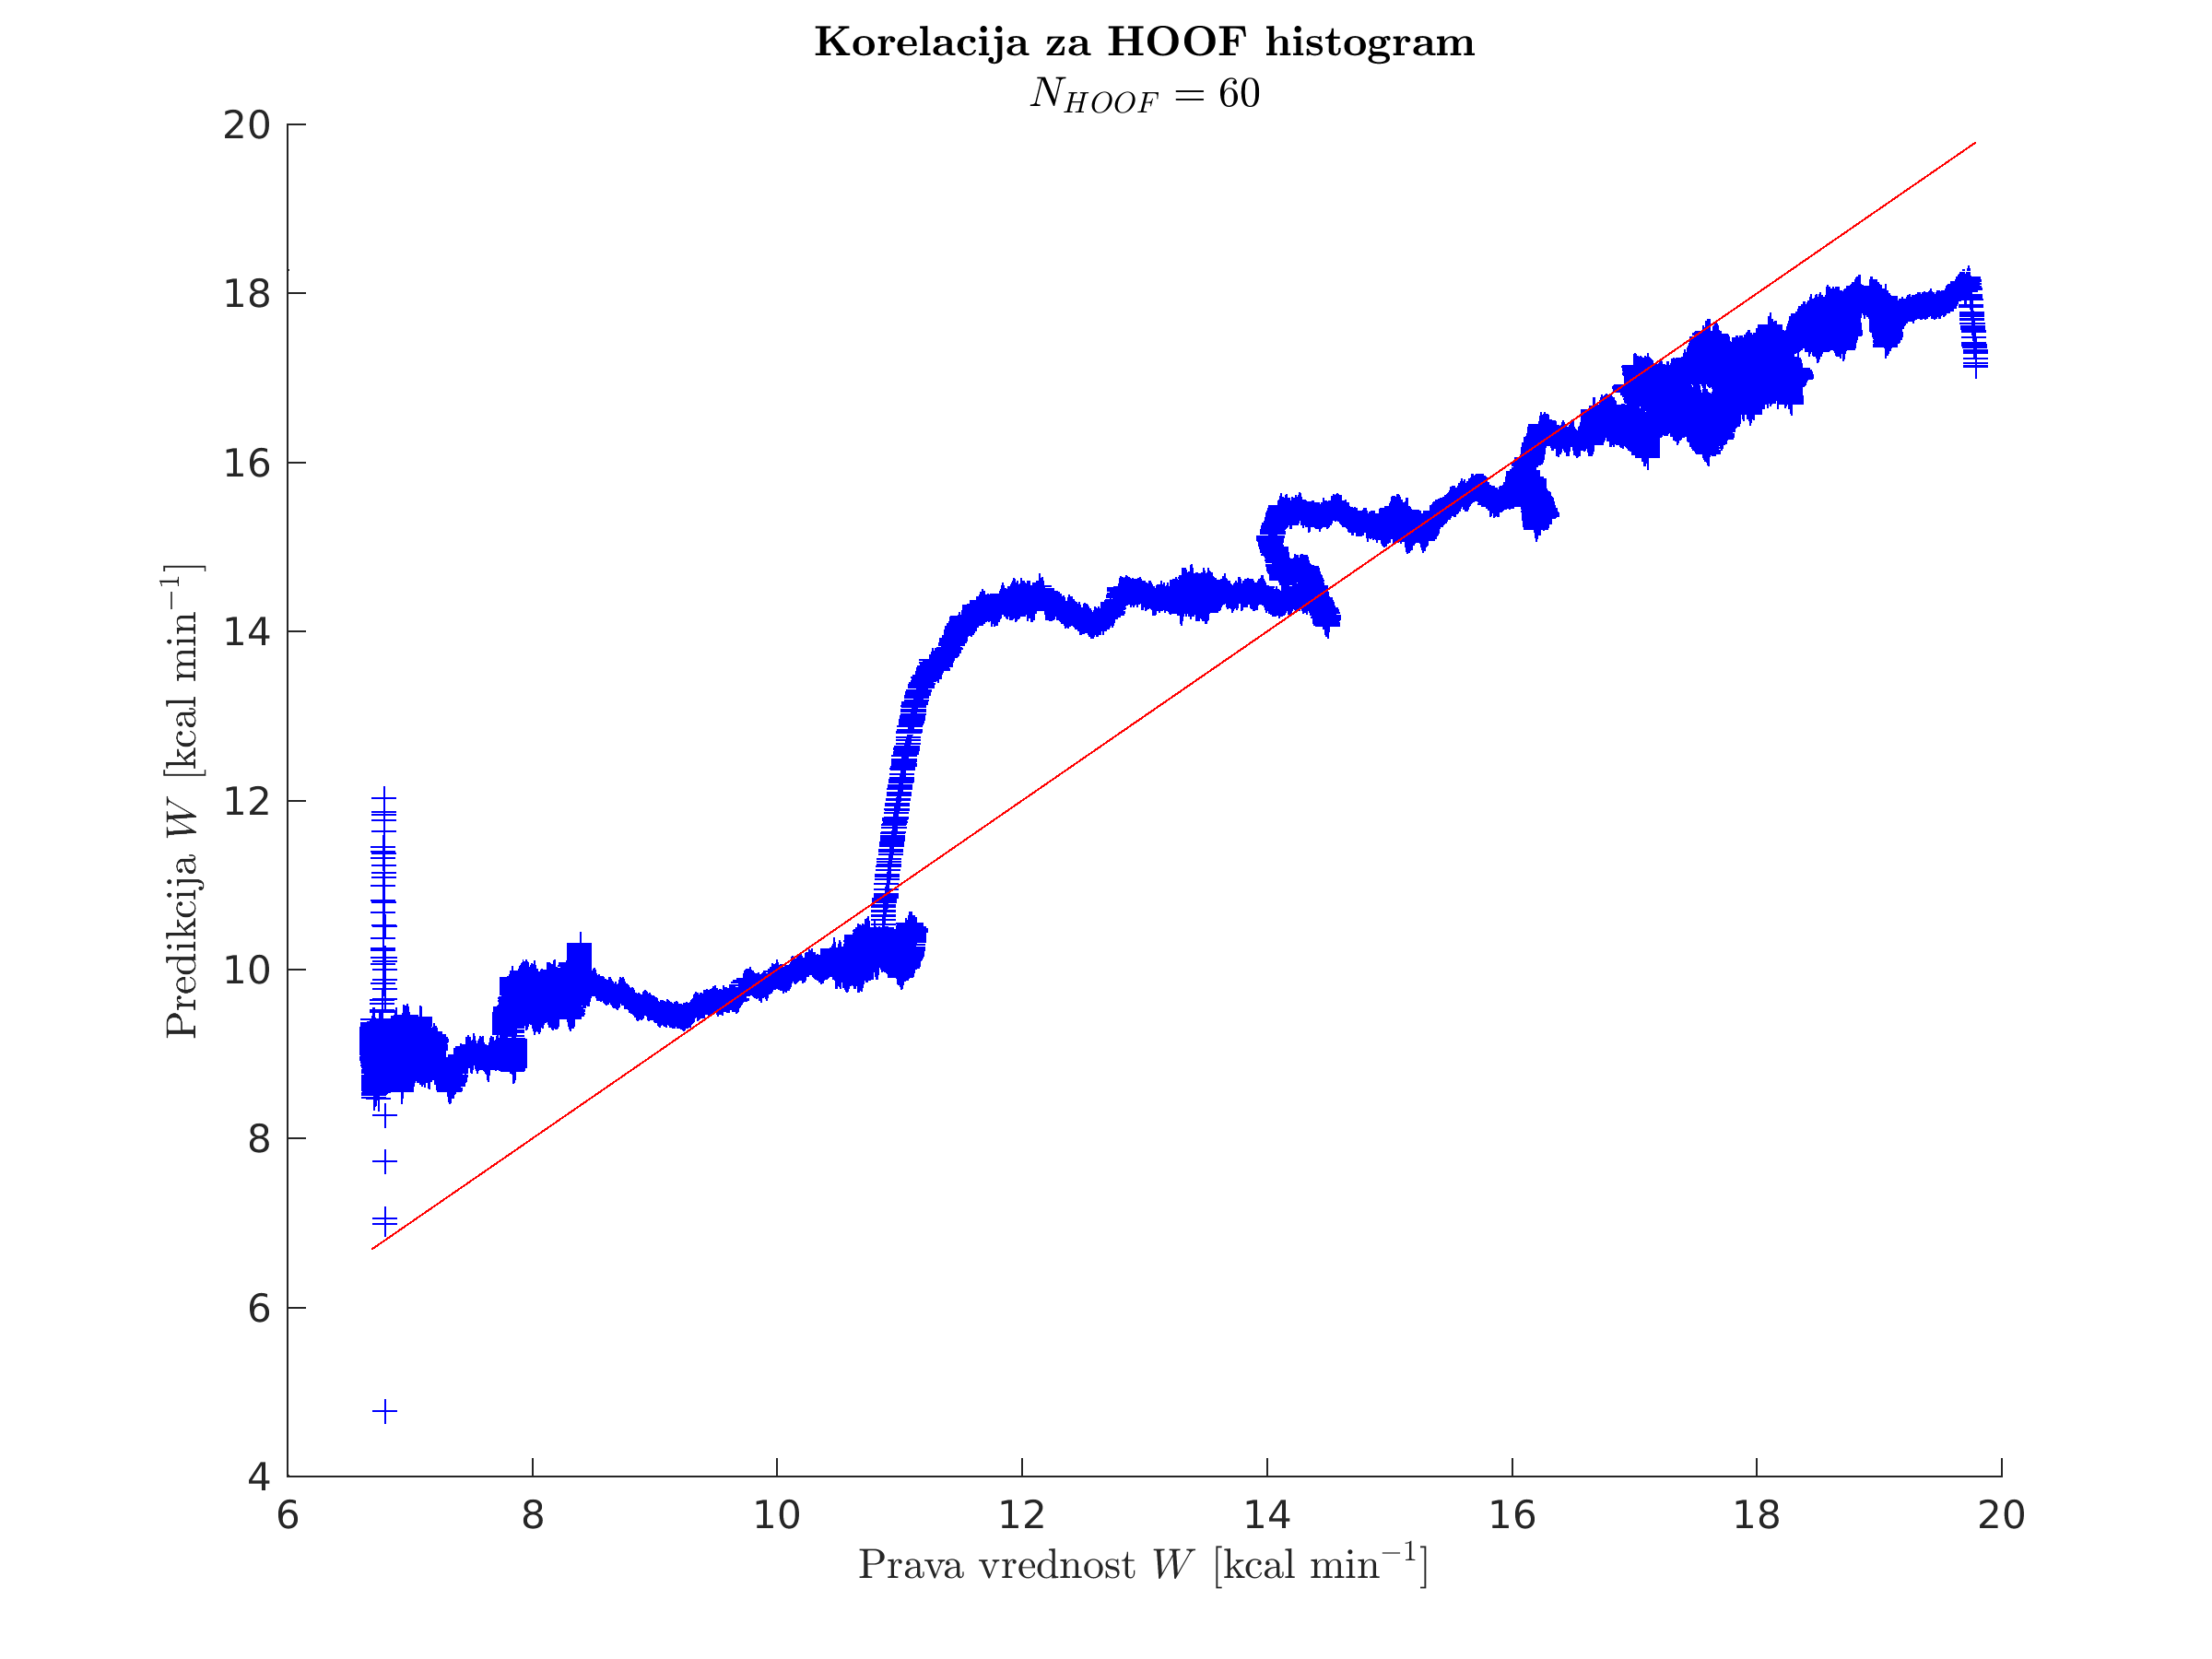
\includegraphics[width=\columnwidth]{./Slike/corr-hoof-60.png}
      \caption{Korelacija $N_{HOOF}=60$.}
      \label{fig:corr-hoof-60}
    \end{subfigure}
    ~
    \begin{subfigure}[b]{0.45\columnwidth}
      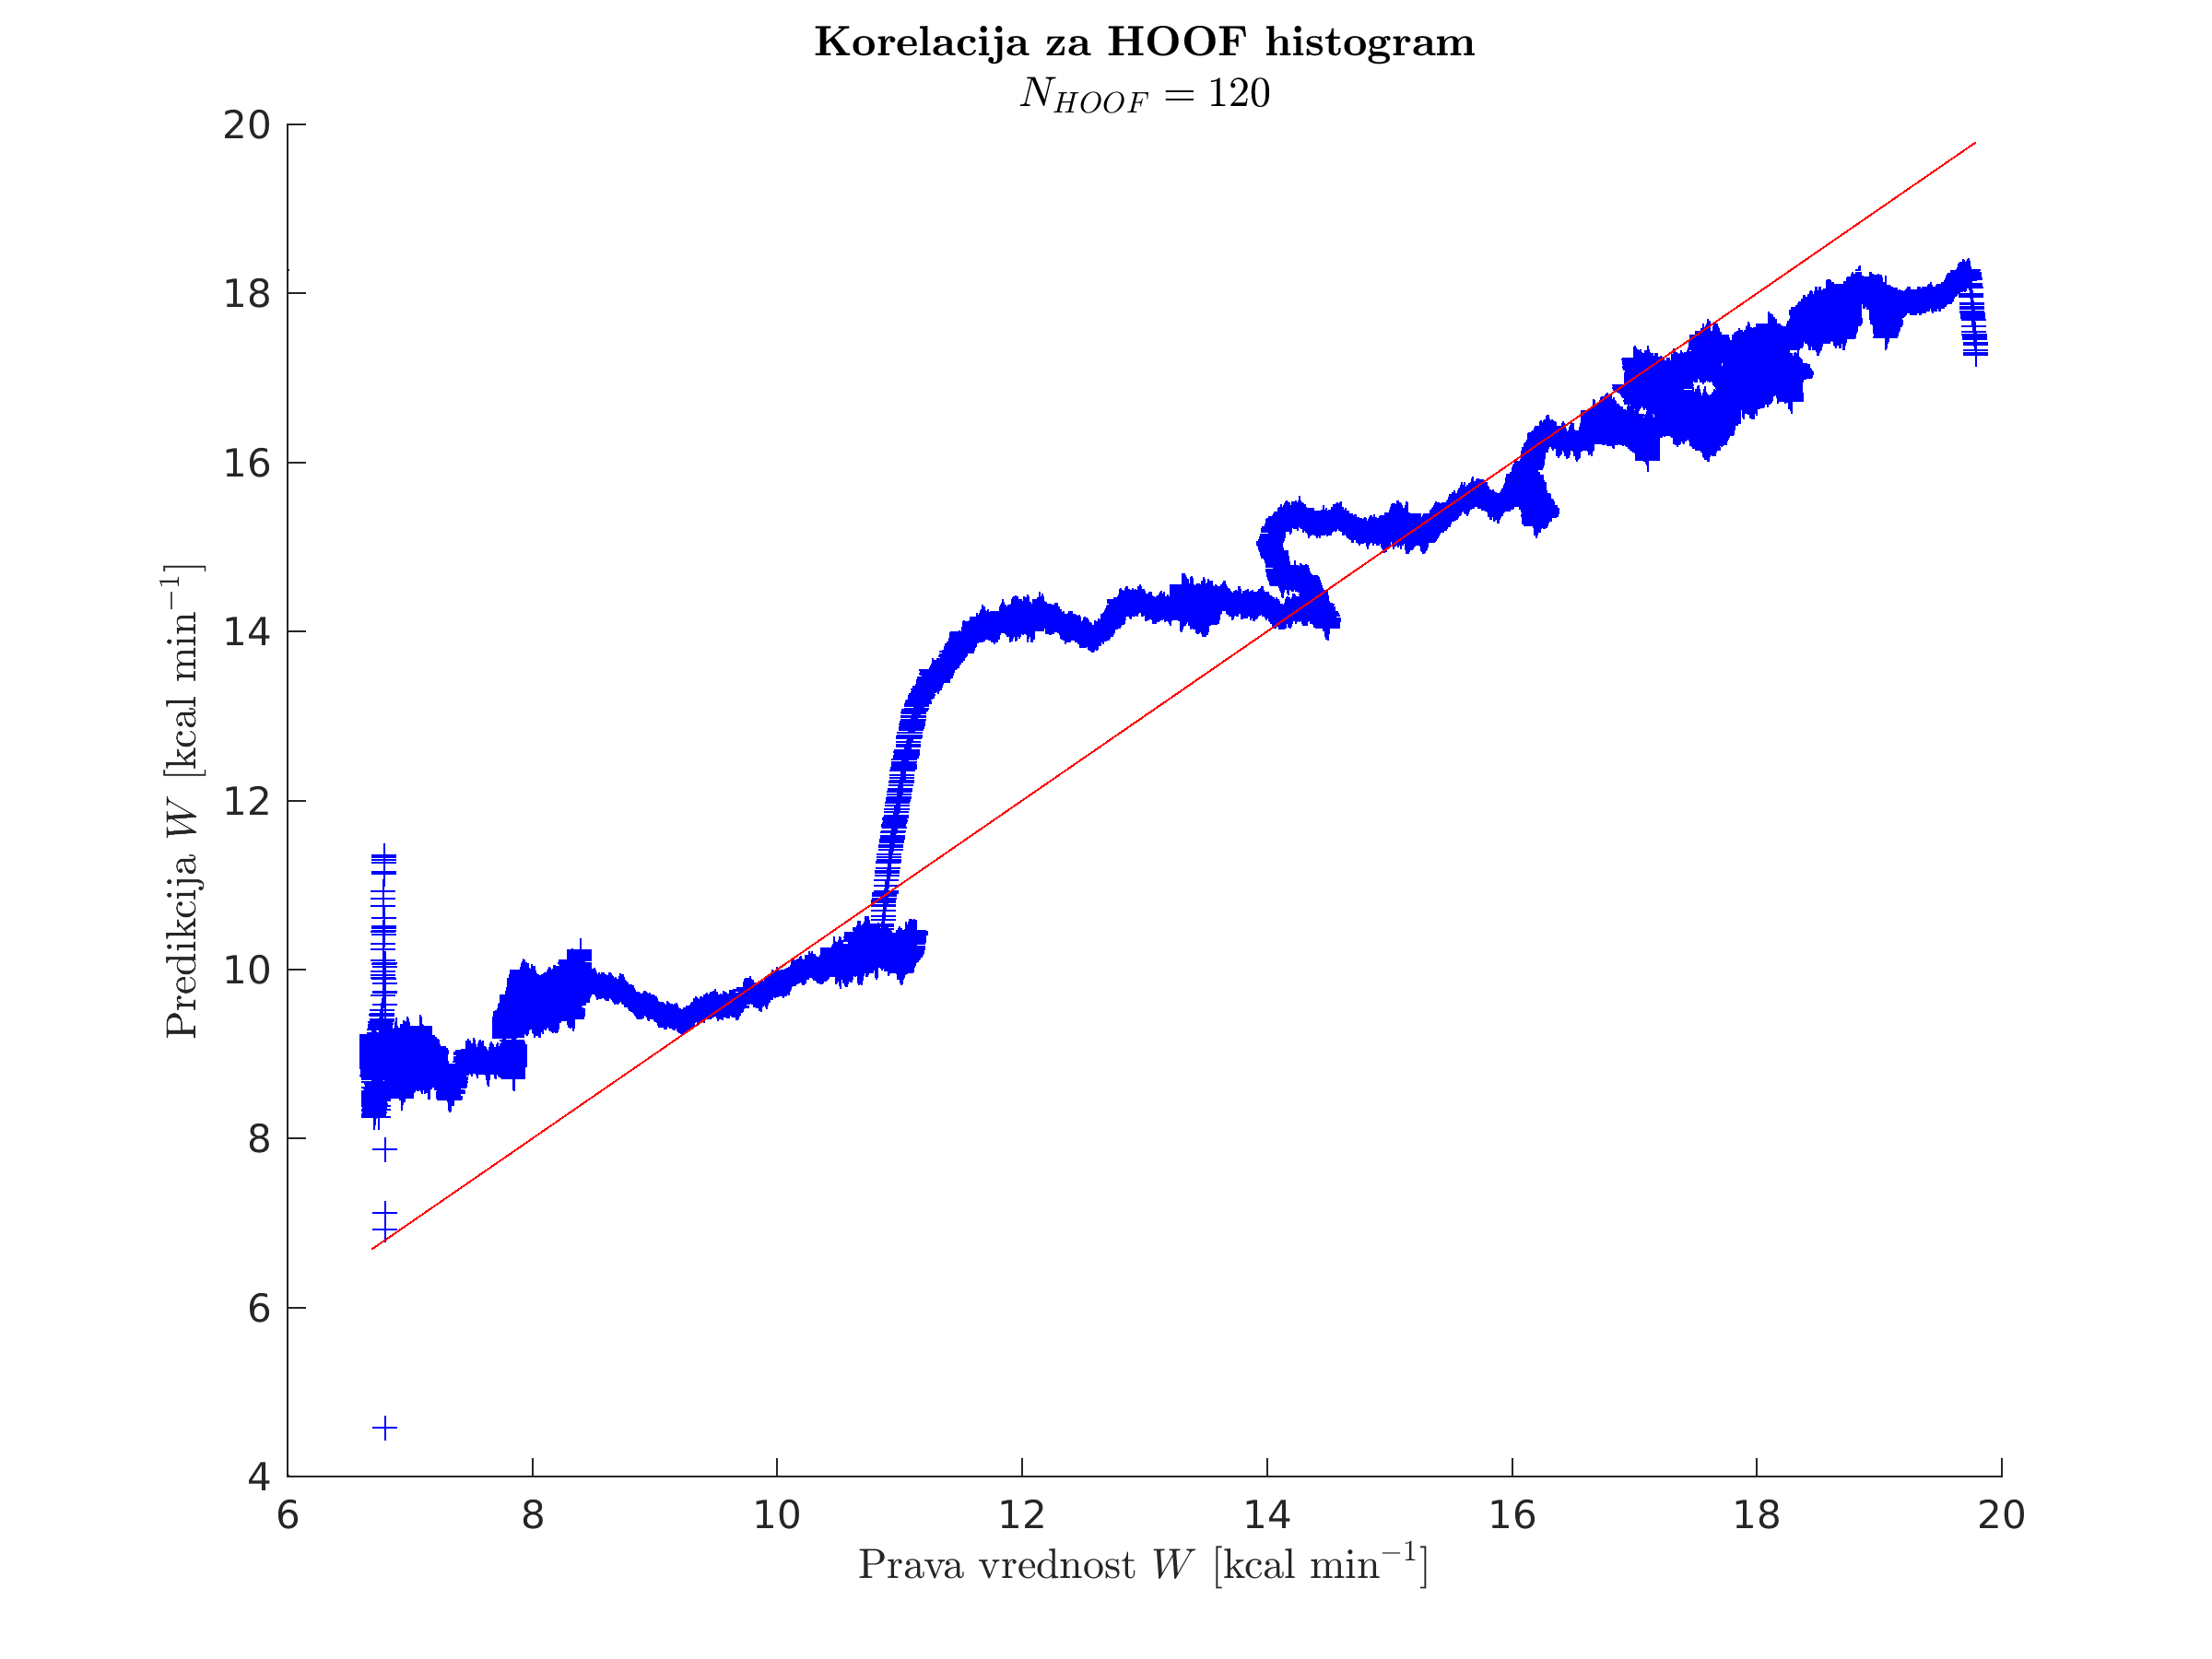
\includegraphics[width=\columnwidth]{./Slike/corr-hoof-120.png}
      \caption{Korelacija $N_{HOOF}=120$.}
      \label{fig:corr-hoof-120}
    \end{subfigure}
    ~
    \begin{subfigure}[b]{0.45\columnwidth}
      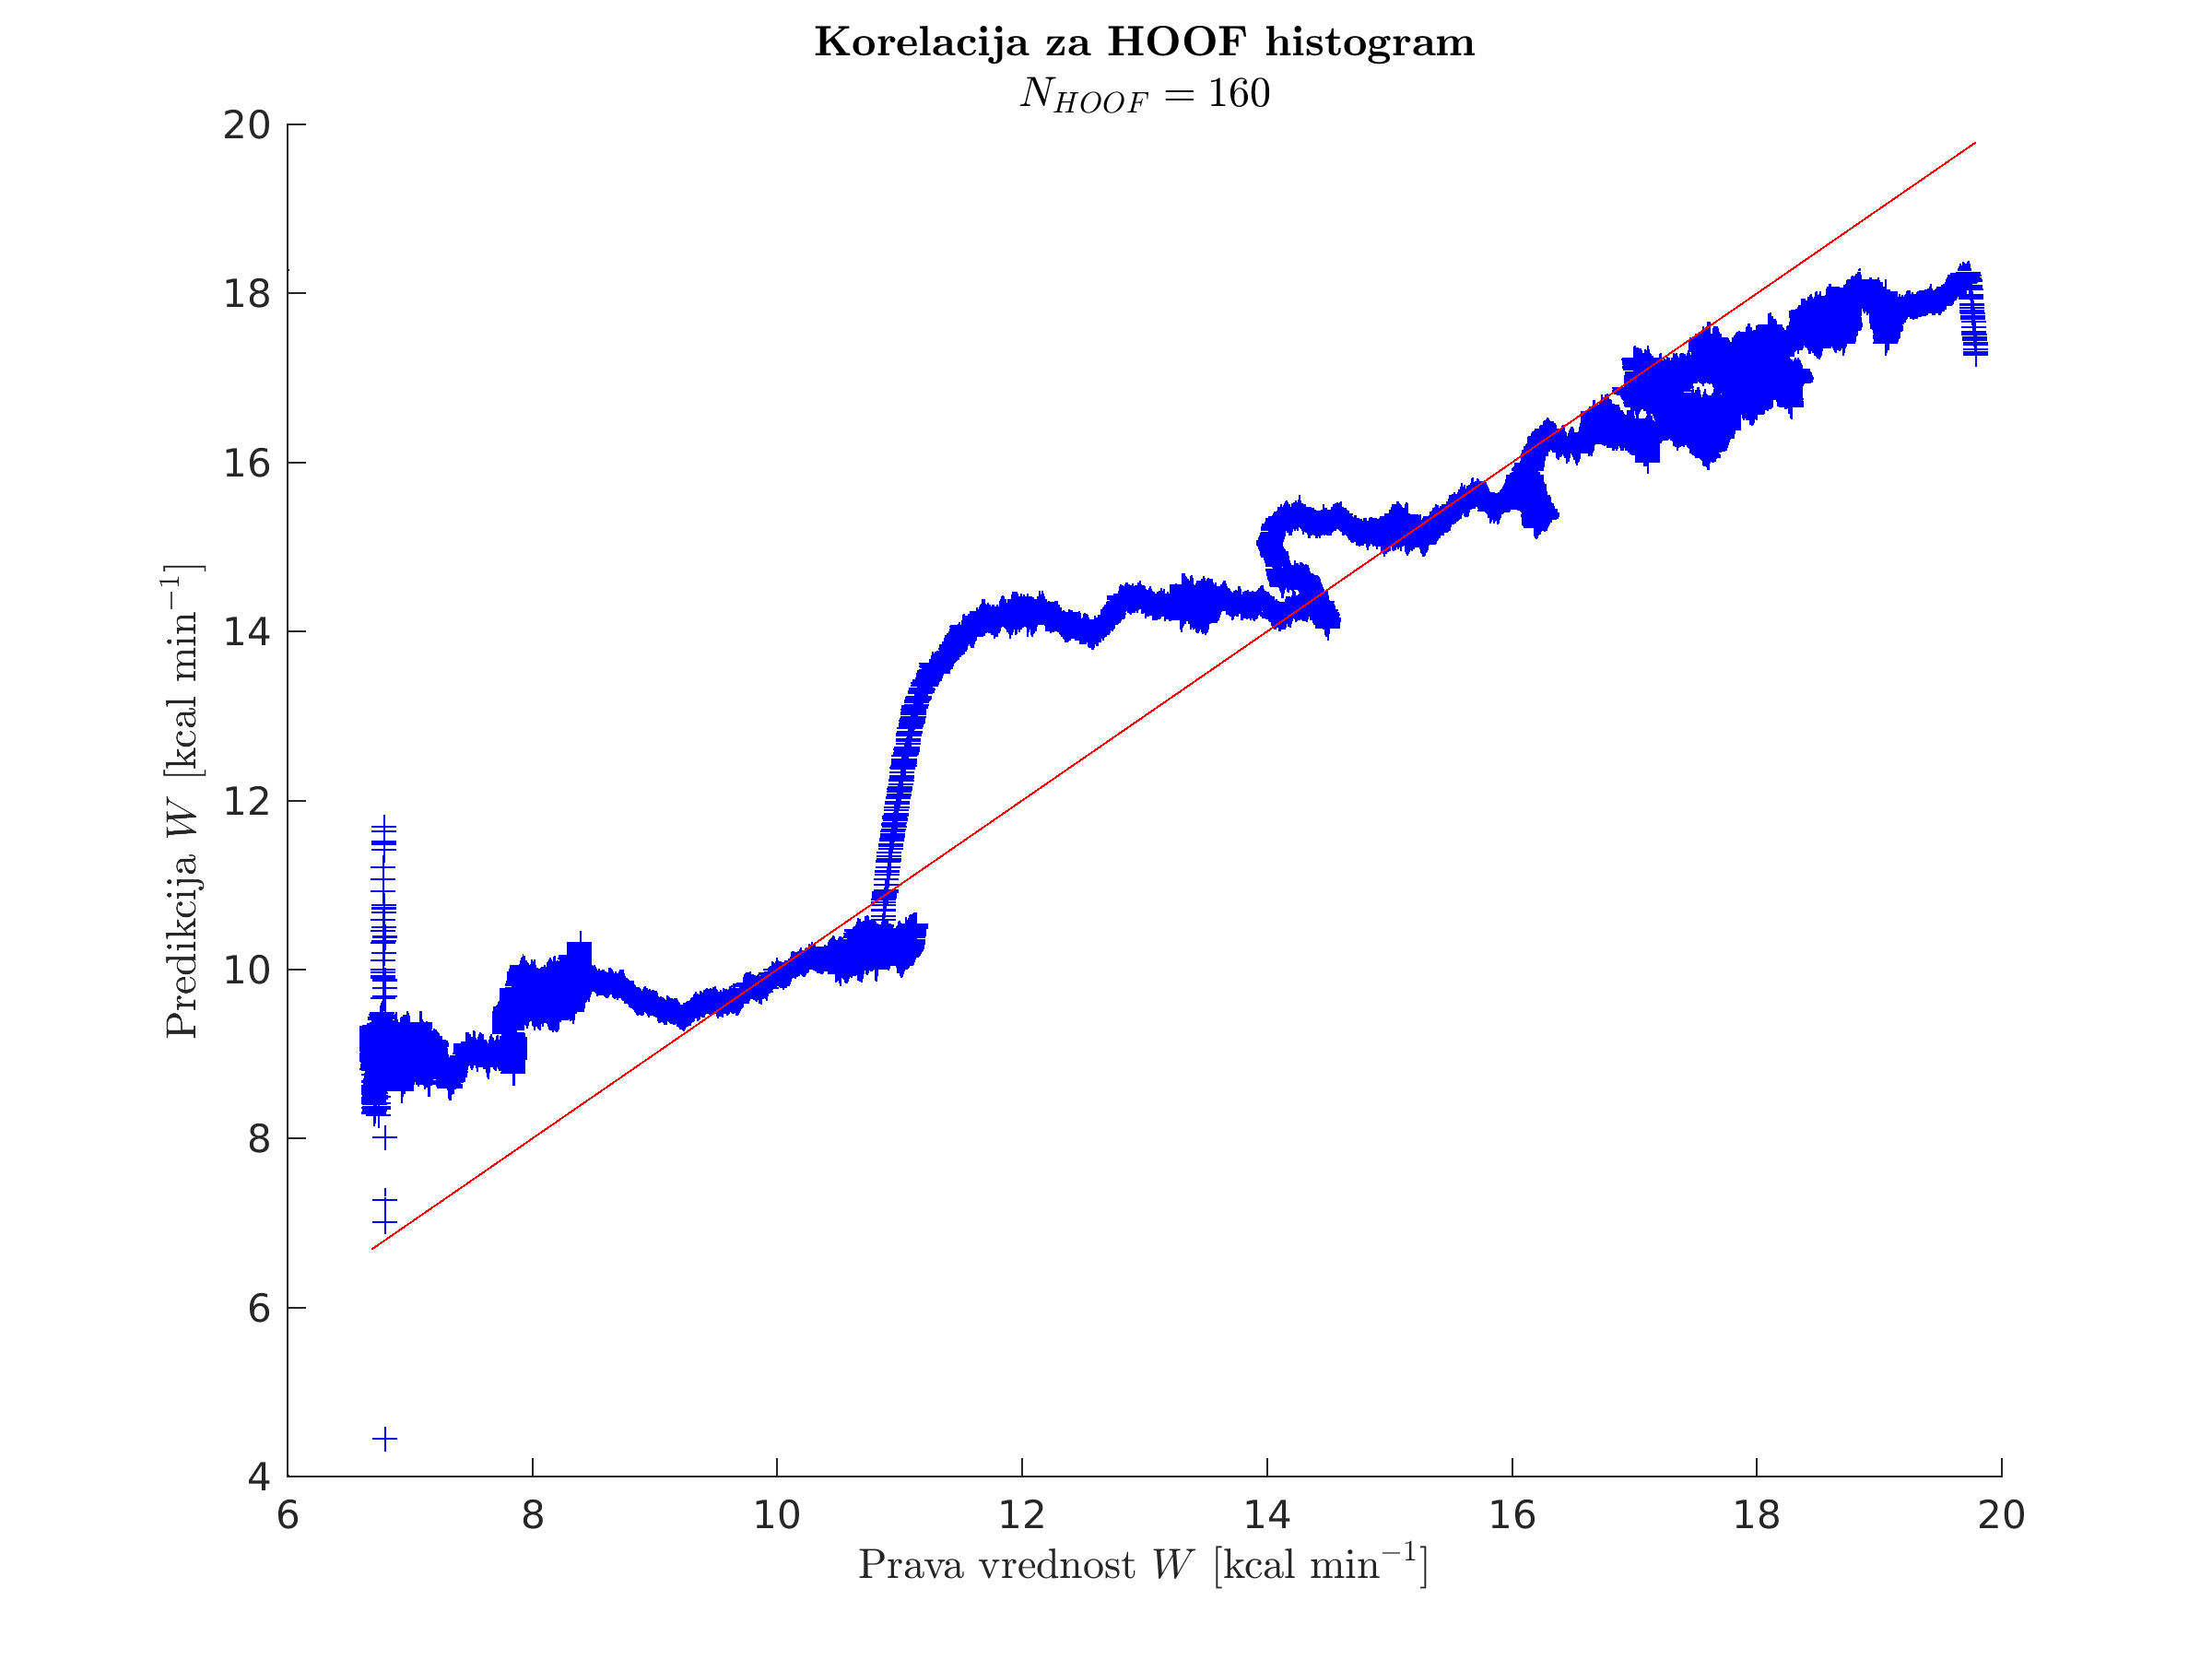
\includegraphics[width=\columnwidth]{./Slike/corr-hoof-160.png}
      \caption{Korelacija $N_{HOOF}=160$.}
      \label{fig:corr-hoof-160}
    \end{subfigure}
    \caption[Grafi korelacij modelov z različnim $N_{HOOF}$]{Grafi korelacij modelov z različnim številom stolpcev $N_{HOOF}$ HOOF deskriptorja. Rezultati so si zelo podobni.}
    \label{fig:corr-hoof}
\end{figure}





\subsection{Optimizacija HAFA deskriptorjev}
Parameter $N_{HAFA}$ smo določili na podlagi rezultatov evaluacije v tabeli \ref{tab:nhafa} in grafov korelacije med referenčnimi podatki in predikcijo \ref{fig:corr-hafa}. Za evaluacijo smo uporabili enak eksperimentalni protokol kot za HOOF značilke v poglavju \ref{sec:hoof}, s to razliko, da smo značilke normirali na intervalu $[0, 1]$ in odstranili stolpec z amplitudami $0.5$. S tem smo odstranili šum, ki se je pojavil, ko ni bilo nobenega gibanja. Amplitudo šuma smo določili, kot maksimalno vrednost amplitude, ki še ni predstavljala gibanja. Optimalni parametri evaluacijske metode so predstavljeni v tabeli \ref{tab:nhafa-param}.


\begin{table}[htb]
	\centering
    \begin{tabular}{S[table-format=2.0] S[table-format=2.3] S[table-format=1.3]  S[table-format=1.3] S[table-format=1.3]}
    \toprule
    \thead{$\mathbf{N_{HAFA}}$} & \thead{$\mathbf{C}$} & \thead{$\mathbf{\gamma}$} & \thead{$\mathbf{\epsilon}$} & \thead{MSE} \\ 
    \midrule
    30 & 8 & 5.657 & 0.616 & 4.329 \\
    60 & 8 & 5.657 & 0.616 & 4.327 \\
    120 & 8 & 5.657 & 0.616 & 4.327 \\
    160 & 8 & 5.657 & 0.616 & 4.327 \\
    \bottomrule
    \end{tabular}
    \caption[Optimalni parameteri RBF jedra modelov za določitev $N_{HAFA}$]{Optimalni parametri RBF jedra za modele z različnim številom stolpcev $N_{HAFA}$ v HAFA deskriptorju.}
    \label{tab:nhafa-param}
\end{table}

V tabeli \ref{tab:nhafa} lahko vidimo, da so rezultati praktično enaki. Za našo metodo smo izbrali $N_{HAFA}=60$, kar v grobem predstavlja $60$ različnih hitrosti z maksimalno amplitudo \SI{60}{px.f^{-1}}.

\begin{table}[htb]
	\centering
    \begin{tabular}{S[table-format=2.0] S[table-format=1.3] S[table-format=1.3] S[table-format=1.3] S[table-format=2.2]}
    \toprule
    \thead{$\mathbf{N_{HAFA}}$} & \thead{$\mathbf{r}$} & \thead{RAE} & \thead{RRSE} & \thead{nSV [\%]}\\
    \midrule%nSV
    30 & 0.984 & 0.213 & 0.231 & 62.08 \\%17879/28799
    \boldentry{2.0}{60} & \boldentry{1.3}{0.984} & \boldentry{1.3}{0.211} & \boldentry{1.3}{0.228} & \boldentry{2.2}{62.60} \\%18028
    120 & 0.984 & 0.211 & 0.228 & 62.63 \\%18037
    160 & 0.984 & 0.211 & 0.228 & 62.63 \\%18037
    \bottomrule
    \end{tabular}
    \caption[Rezultati evaluacije modelov z različnim $N_{HAFA}$]{Rezultati evaluacije modelov z različnim številom stolpcev $N_{HAFA}$ HAFA deskriptorja. Optimalni rezultati so odebeljeni.}
    \label{tab:nhafa}
\end{table}

\begin{figure}[htb]
	\centering
    \begin{subfigure}[t]{0.45\columnwidth}
    	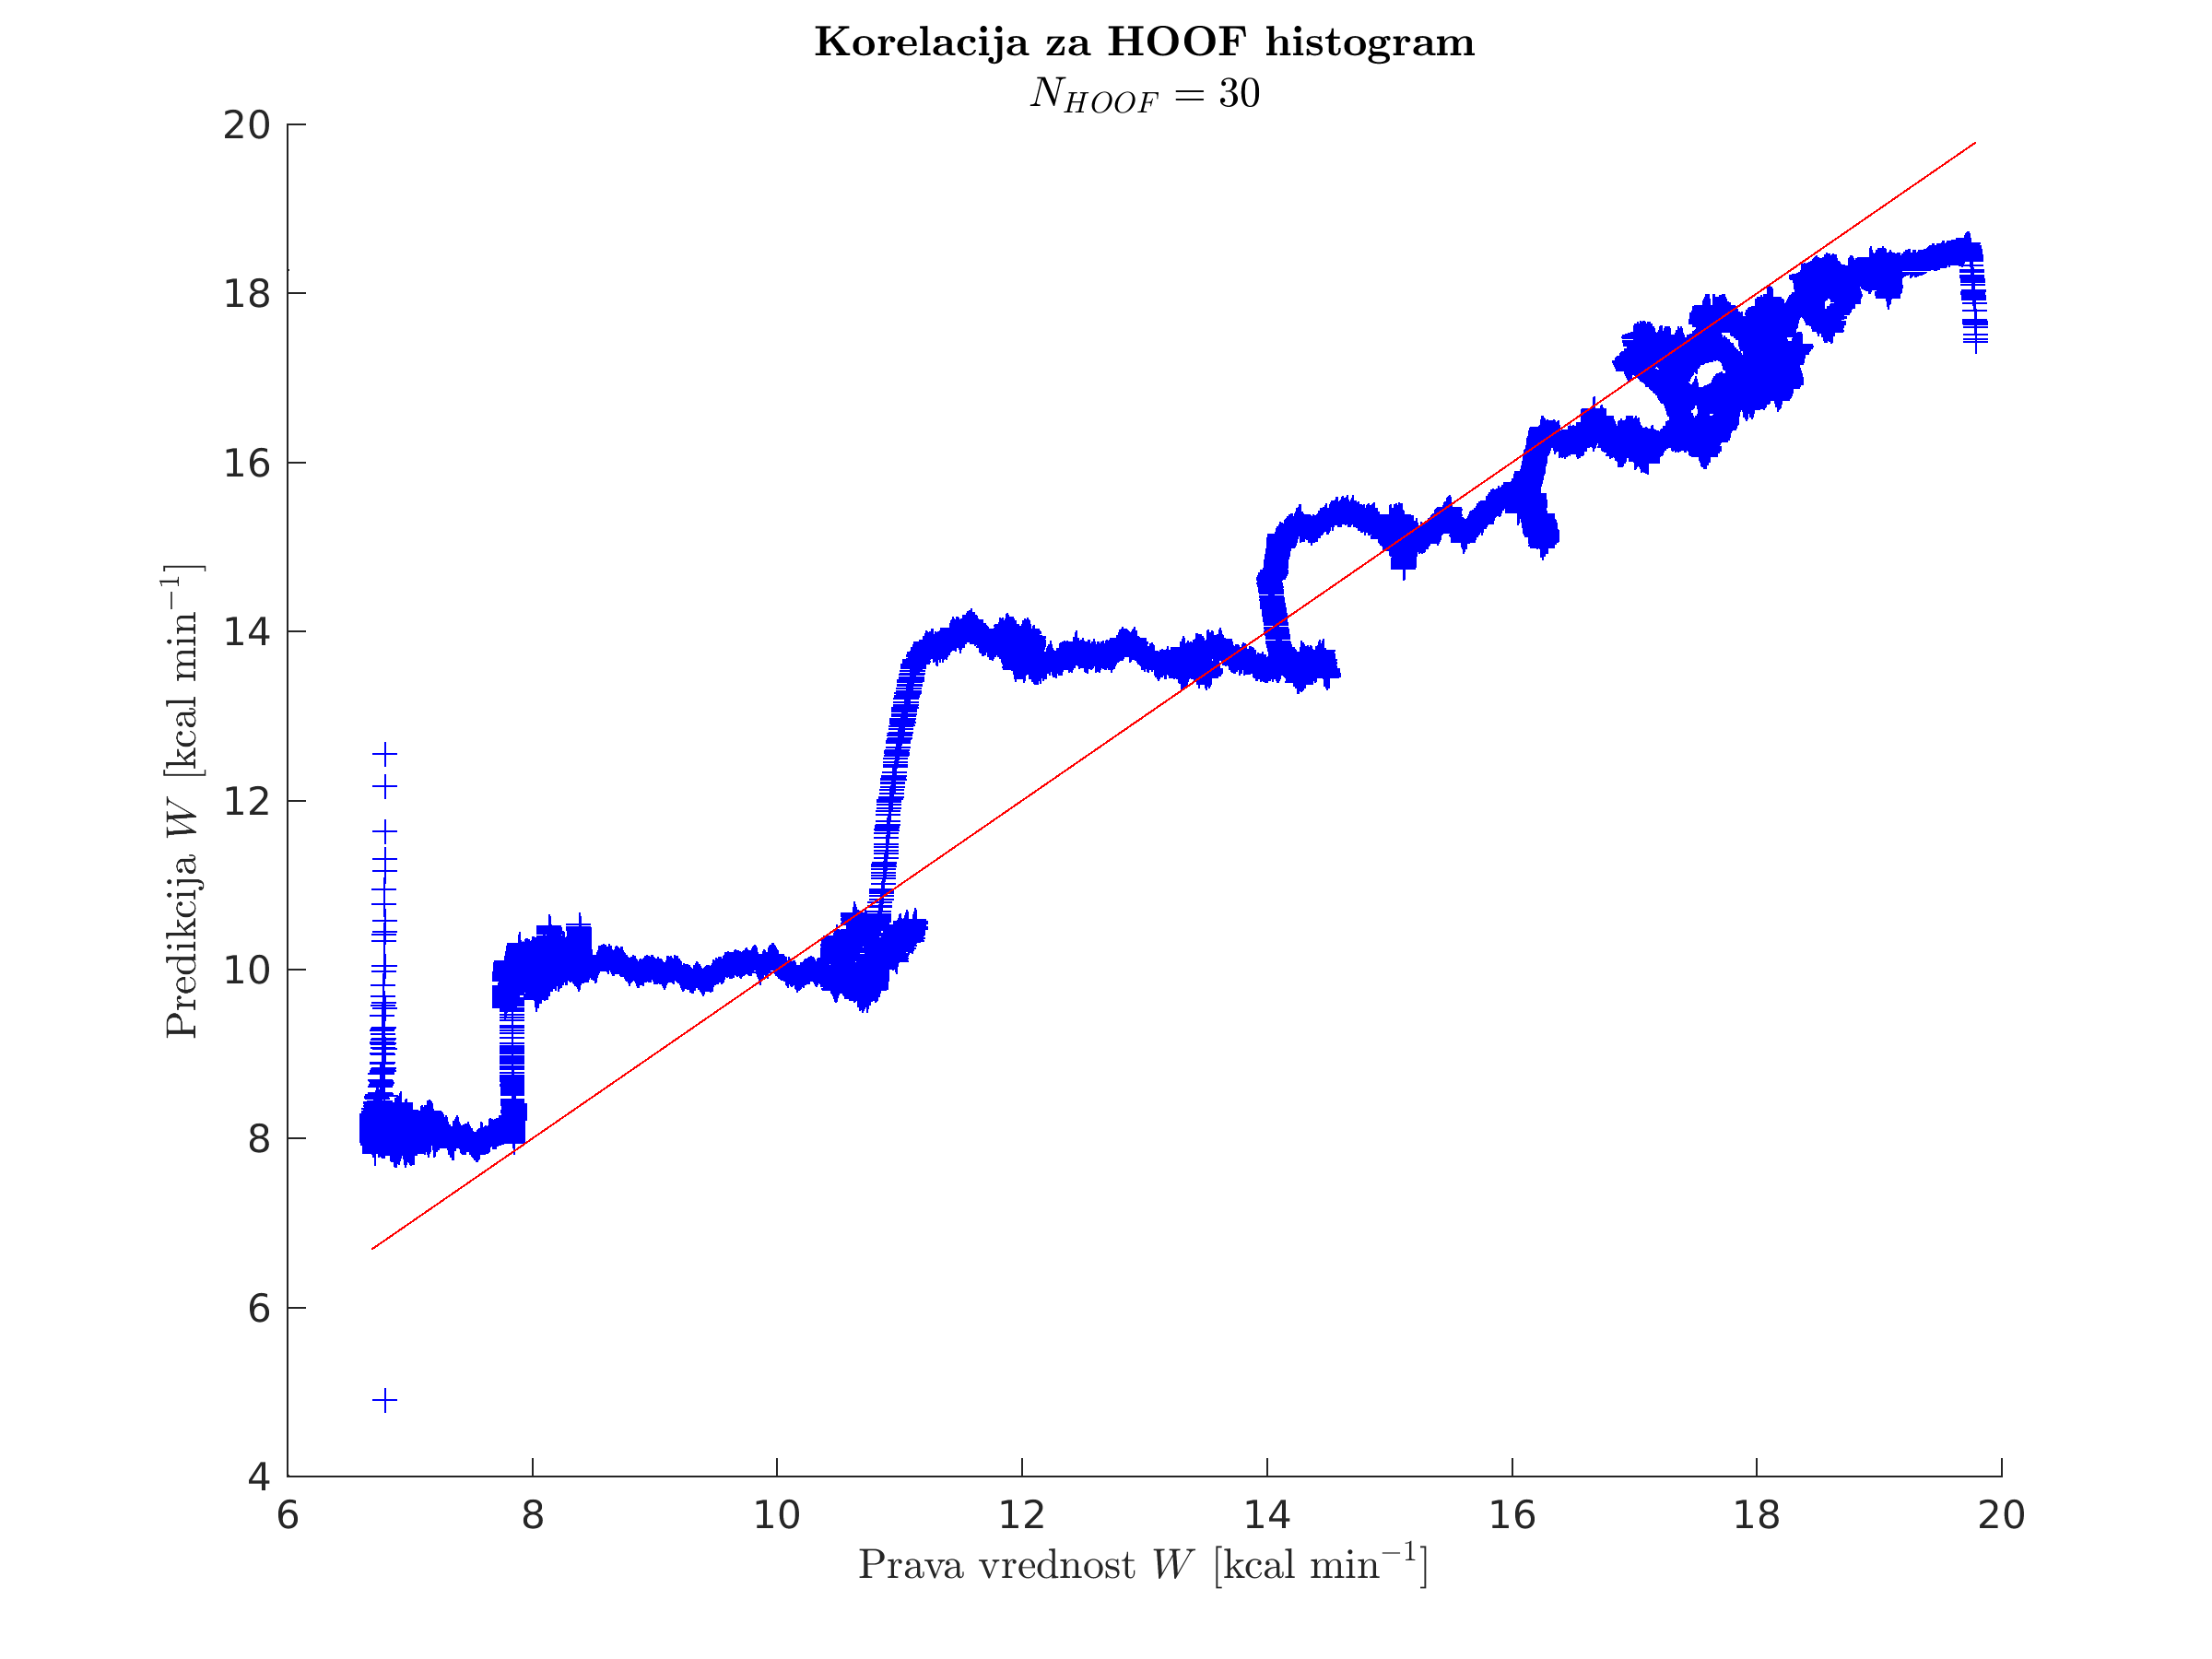
\includegraphics[width=\columnwidth]{./Slike/corr-hafa-30.png}
        \caption{Korelacija $N_{HAFA}=30$.}
        \label{fig:corr-hafa-30}
    \end{subfigure}
    ~
    \begin{subfigure}[t]{0.45\columnwidth}
      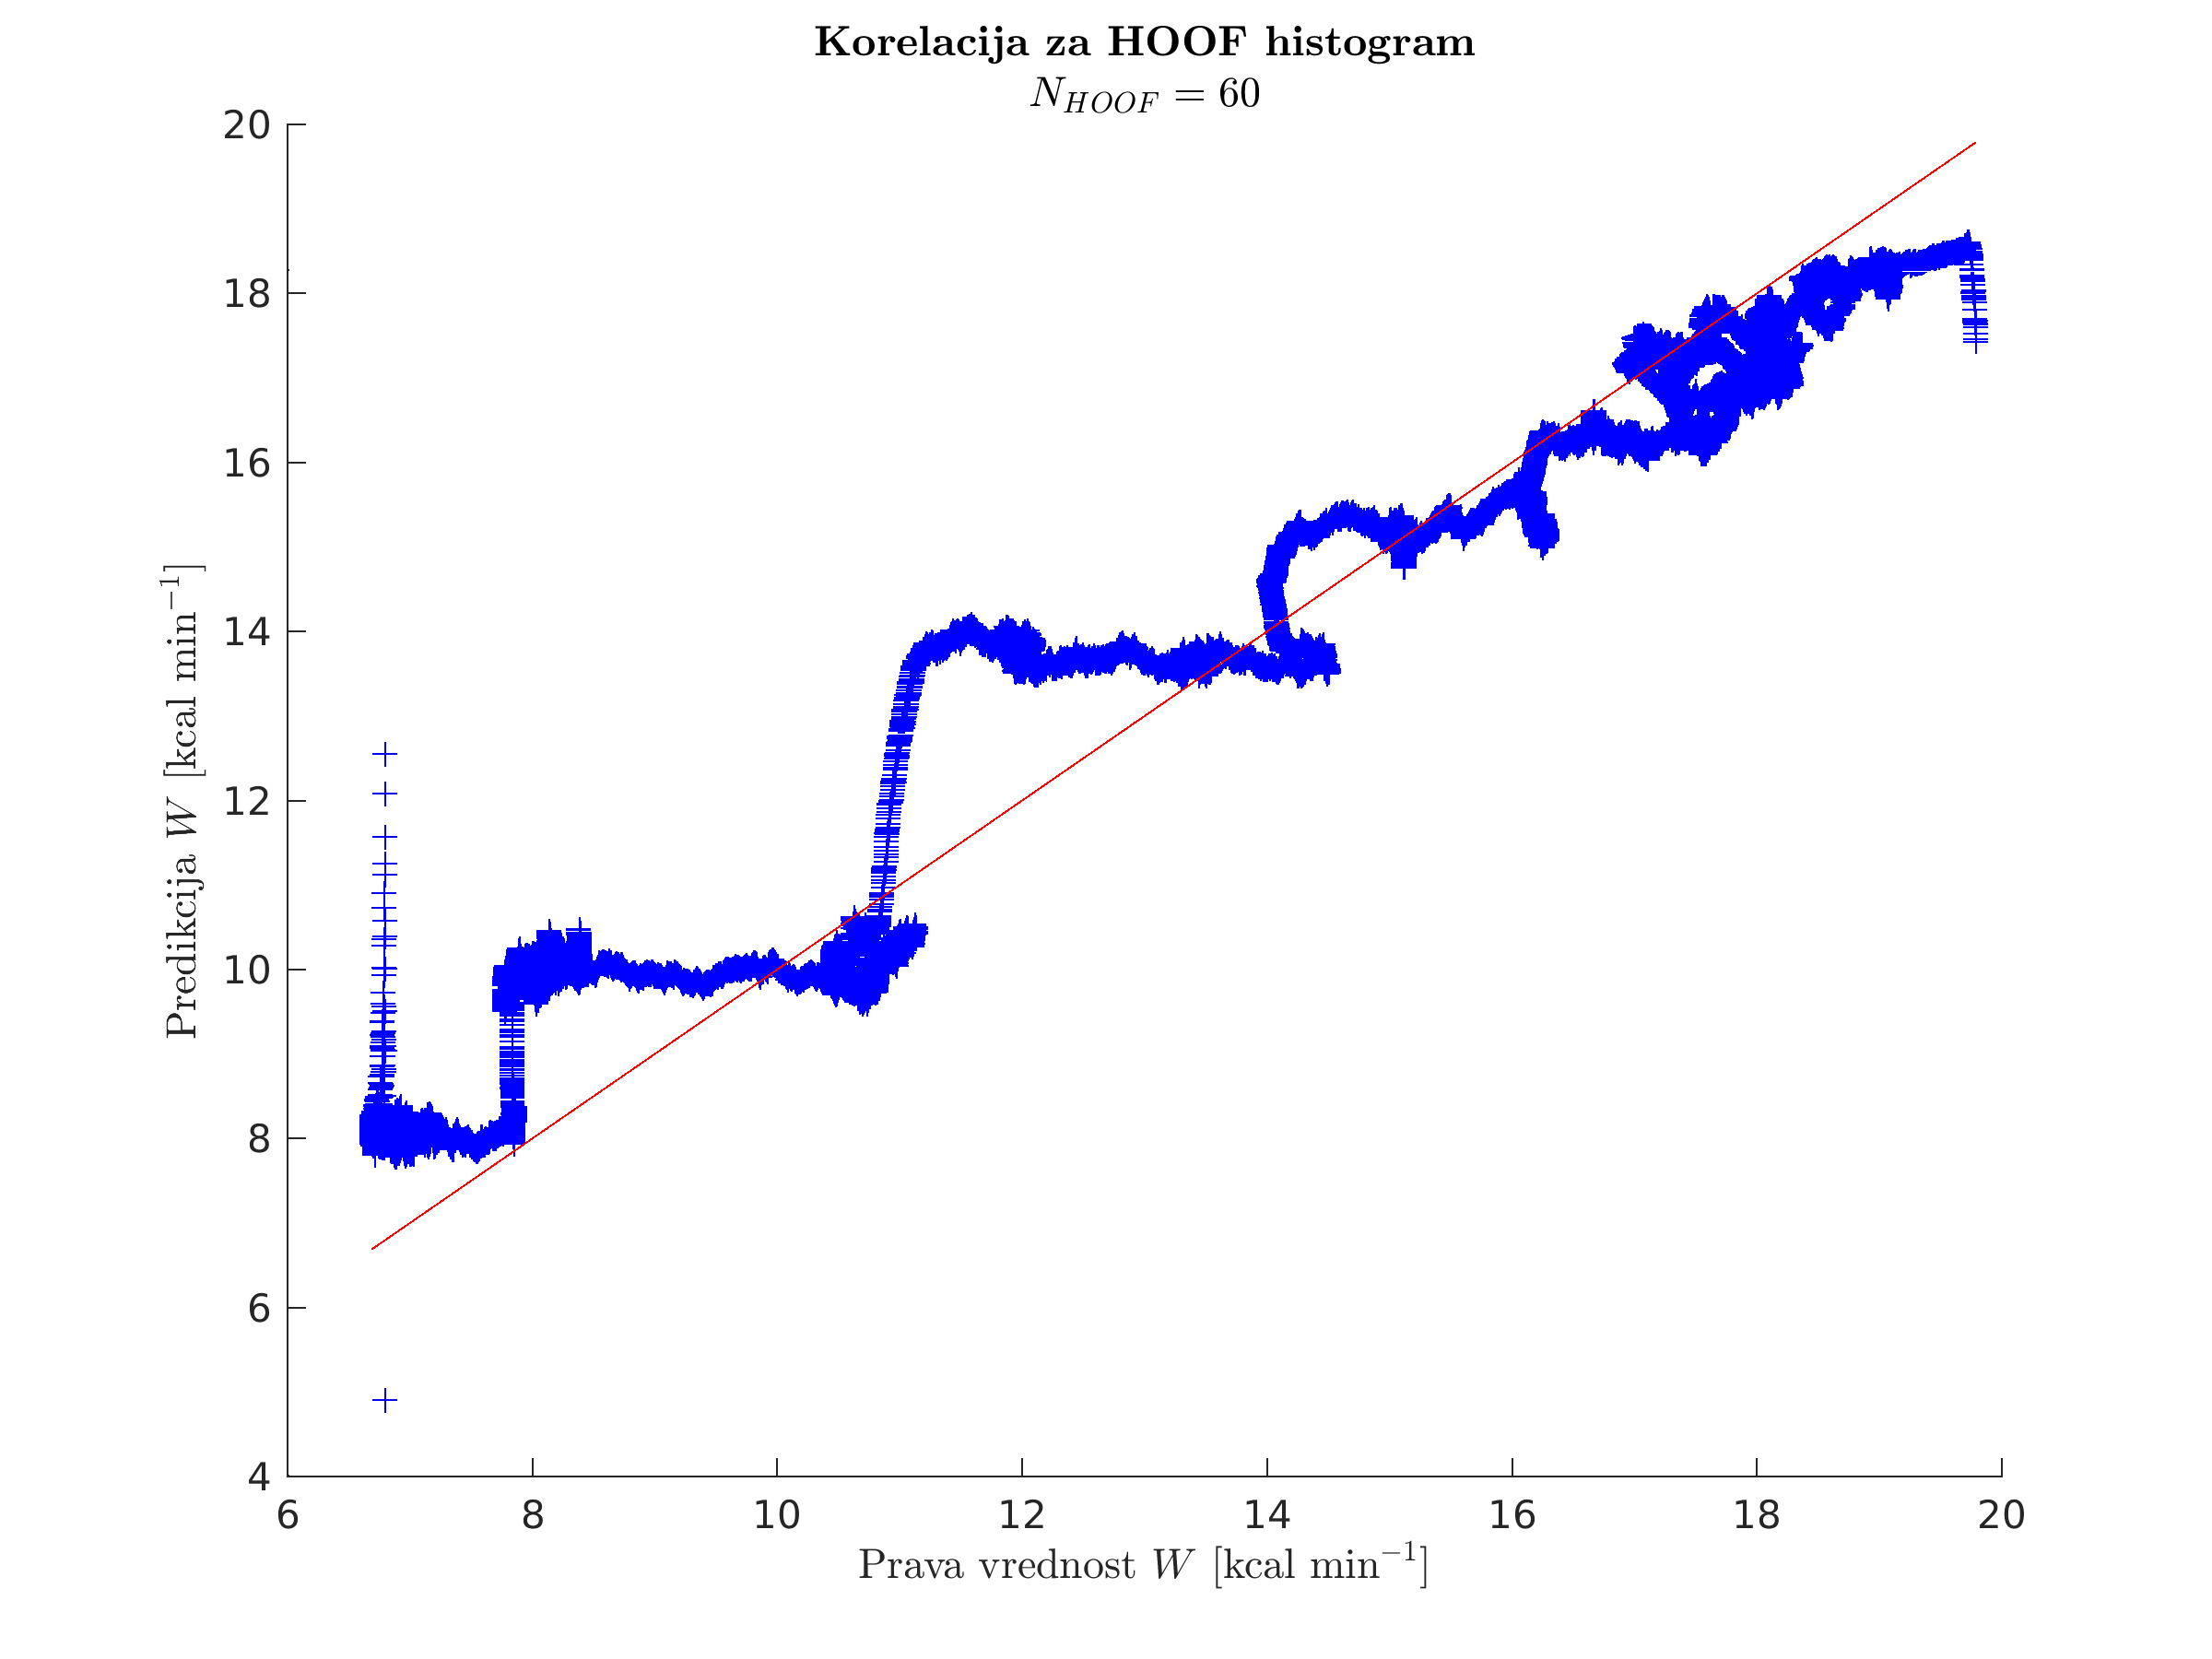
\includegraphics[width=\columnwidth]{./Slike/corr-hafa-60.png}
      \caption{Korelacija $N_{HAFA}=60$.}
      \label{fig:corr-hafa-60}
    \end{subfigure}
    ~
    \begin{subfigure}[b]{0.45\columnwidth}
      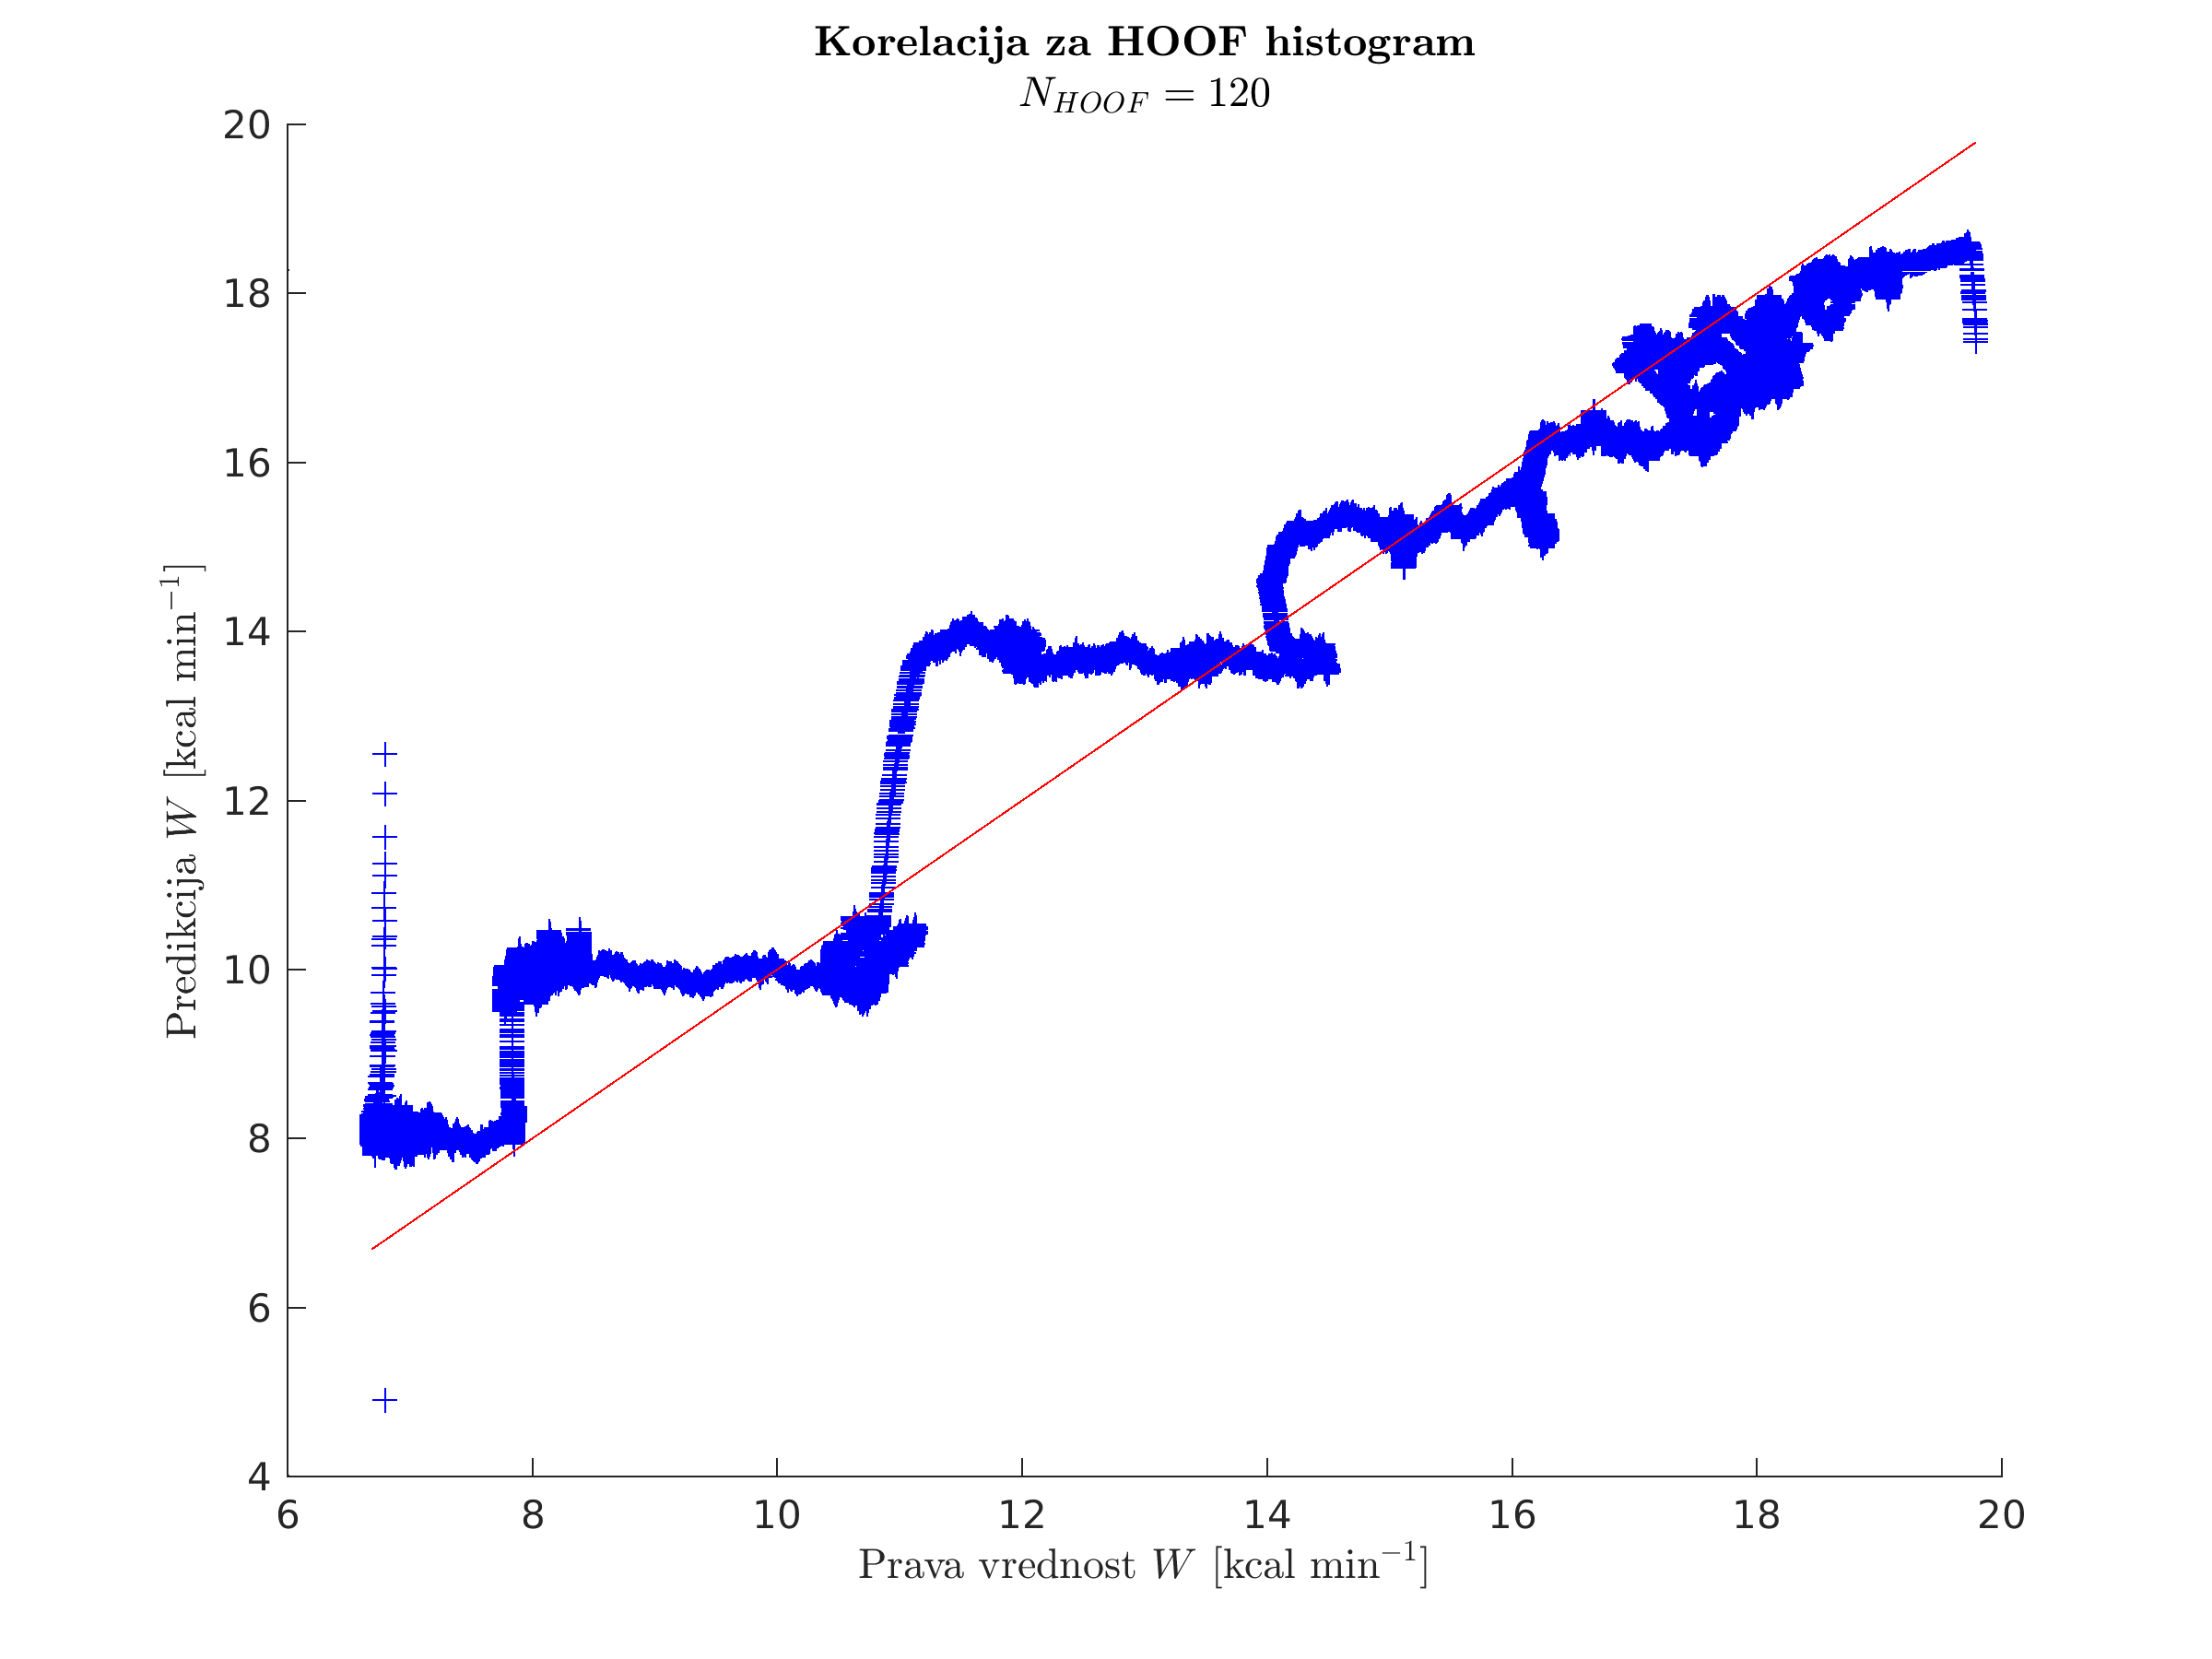
\includegraphics[width=\columnwidth]{./Slike/corr-hafa-120.png}
      \caption{Korelacija $N_{HAFA}=120$.}
      \label{fig:corr-hafa-120}
    \end{subfigure}
    ~
    \begin{subfigure}[b]{0.45\columnwidth}
      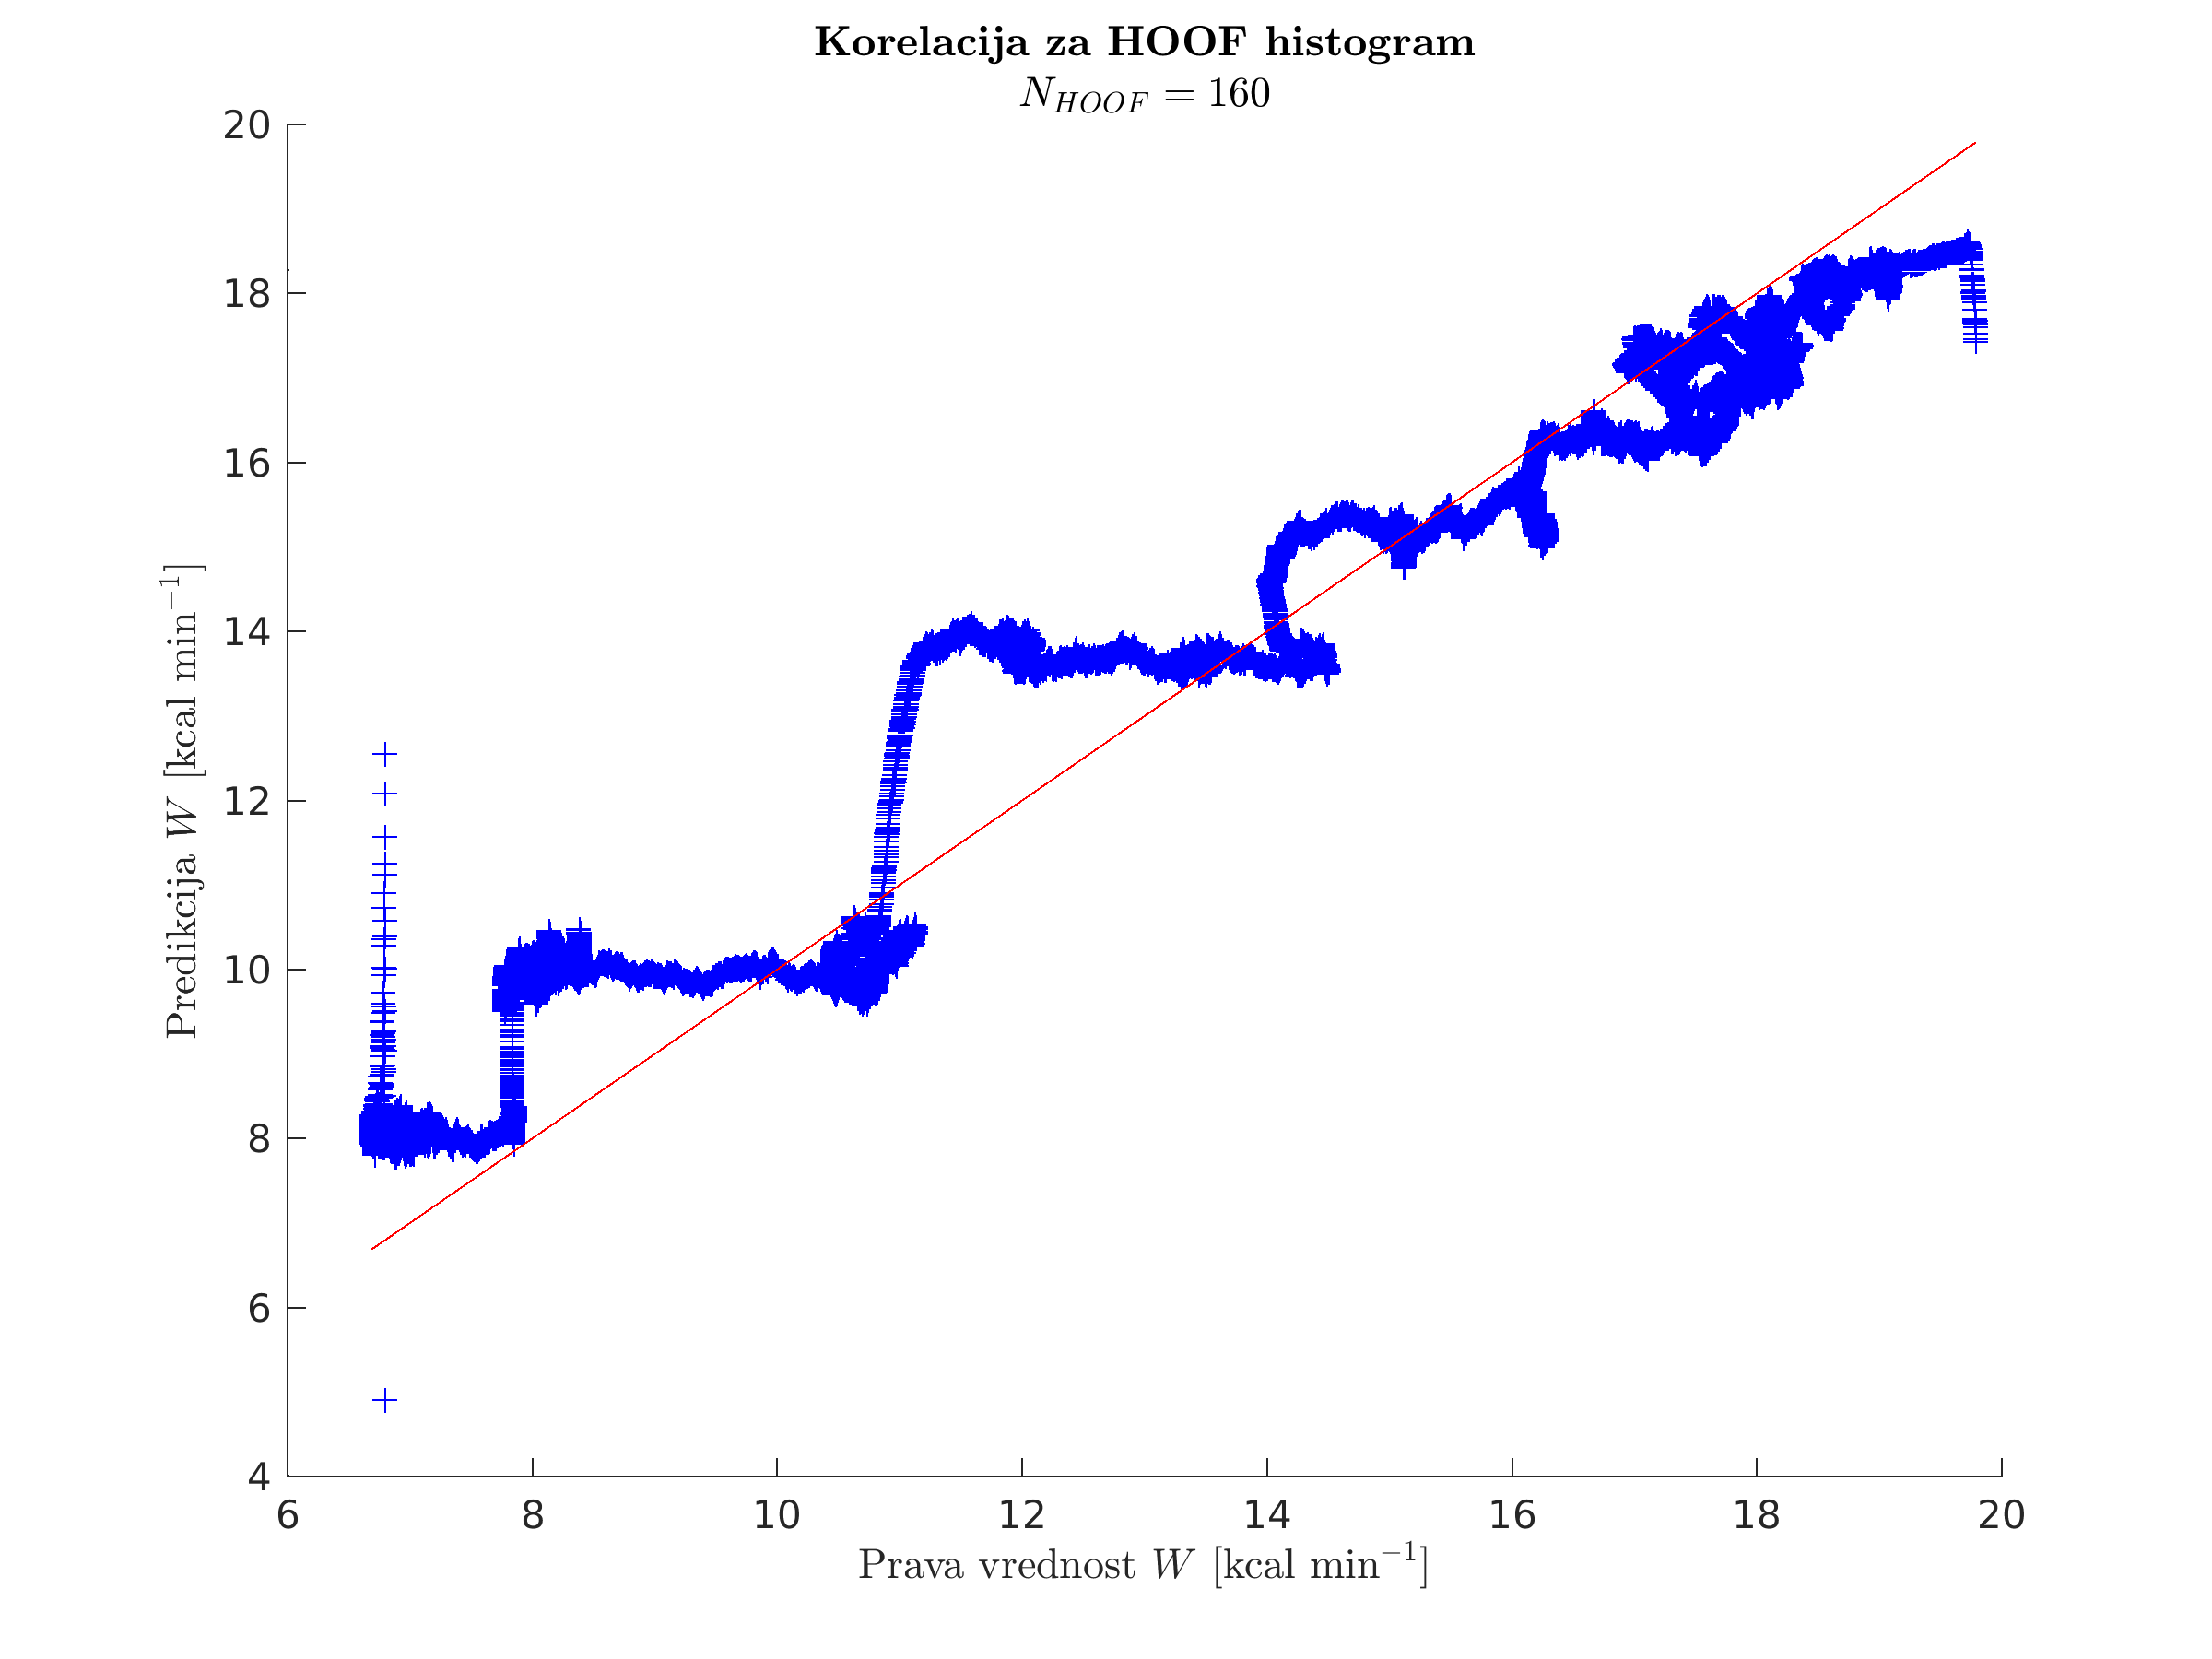
\includegraphics[width=\columnwidth]{./Slike/corr-hafa-160.png}
      \caption{Korelacija $N_{HAFA}=160$.}
      \label{fig:corr-hafa-160}
    \end{subfigure}
    \caption[Grafi korelacij modelov z različnim $N_{HAFA}$]{Grafi korelacij modelov z različnim številom stolpcev $N_{HAFA}$ HAFA deskriptorja. Rezultati so si zelo podobni.}
    \label{fig:corr-hafa}
\end{figure}



\subsection{Normalizacija HAFA deskriptorjev}
% Zakaj naj bi bila ta rešitev dobra
% teorija tovrstne kalibracije
% Kako s to kalibracijo nismo popravili stvari
% In da smo ugotovili da obstaja še prostorski tok, ki bi nam rešil težave
V praksi se pokaže, da normiran HAFA histogram ne... -> To paše pod eksperimente.




\subsection{Izbira deskriptorjev}

Chaudhry et al. \cite{chaudhry2009histograms} predlaga uporabo histogramov orientiranega optičnega toka (HOOF) za estimacijo gibanja. Vendar pa smo v preliminarnih terenskih testiranjih \cite{koporec2017observation} ugotovili, da njihova uporaba v realnih okoliščinah ni zadovoljiva. HOOF deskriptorju smo pripeli HAFA deskriptor in tako dobili razširjeni deskriptor HOOF-HAFA, ki v splošnem daje boljše rezultate, kot lahko vidimo v tabeli \ref{tab:izbira} in na primerjalnih slikah \ref{fig:izbira}.

Pri evaluaciji deskriptorjev HOOF in HOOF-HAFA smo uporabili učne vzorce hrbtne kamere terenskih testov. Evaluirali smo za podatke srčnega utripa $hr$. Srčni utrip smo za gradnjo modelov pretvorili v energijsko porabo $W$ po enačbi \eqref{eq:charlot}. Pridobljene značilke smo normirali na intervalu [0,1] in jih uporabili za učenje regresijskega modela z metodo podpornih vektorjev $\epsilon$-SVR in jedrom RBF. Za določitev optimalnih parametrov, ki so predstavljeni v tabeli \ref{tab:nhoof-param}, smo uporabili optimizacijsko metodo mrežnega iskanja \cite{hsu2003practical}. Rezultate smo filtrirali še s Gaussovim jedrom (predstavljen v \ref{sec:gaussov-filter}) velikosti $6$ in varianco $\sigma=16$. 

\begin{table}[htb]
	\centering
    \begin{tabular}{l S[table-format=2.3] S[table-format=1.3] S[table-format=1.3] S[table-format=1.3]}
    \toprule
    \textbf{Deskriptor} & \thead{$\mathbf{C}$} & \thead{$\mathbf{\gamma}$} & \thead{$\mathbf{\epsilon}$} & \thead{MSE} \\ 
    \midrule
    HOOF & 2.828 & 11.314 & 0.435 & 2.192 \\
    HOOF-HAFA & 5.657 & 2.828 & 0.154 & 1.781 \\
    \bottomrule
    \end{tabular}
    \caption[Optimalni parameteri RBF jedra modelov za izbiro deskriptorjev]{Optimalni parametri RBF jedra za modele z različnim deskriptorjem.}
    \label{tab:izbira-param}
\end{table}


\begin{table}[htb]
	\centering
    \begin{tabular}{l S[table-format=1.3] S[table-format=1.3] S[table-format=1.3] S[table-format=2.2]}
    \toprule
    \textbf{Deskriptor} & \thead{$\mathbf{r}$} & \thead{RAE} & \thead{RRSE} & \thead{nSV [\%]}\\
    \midrule%nSV
    HOOF & 0.992 & 0.336 & 0.317 & \boldentry{2.2}{82.34} \\%2187/2656
    \textbf{HOOF-HAFA} & \boldentry{1.3}{0.991} & \boldentry{1.3}{0.157} & \boldentry{1.3}{0.205} & 89.53 \\%2378
    \bottomrule
    \end{tabular}
    \caption[Rezultati evaluacije modelov z različnim deskriptorjem]{Rezultati evaluacije modelov z različnim deskriptorjem. Optimalni rezultati so odebeljeni. Vidimo lahko, da se bolje odnese razširjeni deskriptor HOOF-HAFA, čeprav model uporablja več podpornih vektorjev. }
    \label{tab:izbira}
\end{table}



\begin{figure}[htb]
	\centering
    \begin{subfigure}[t]{0.45\columnwidth}
      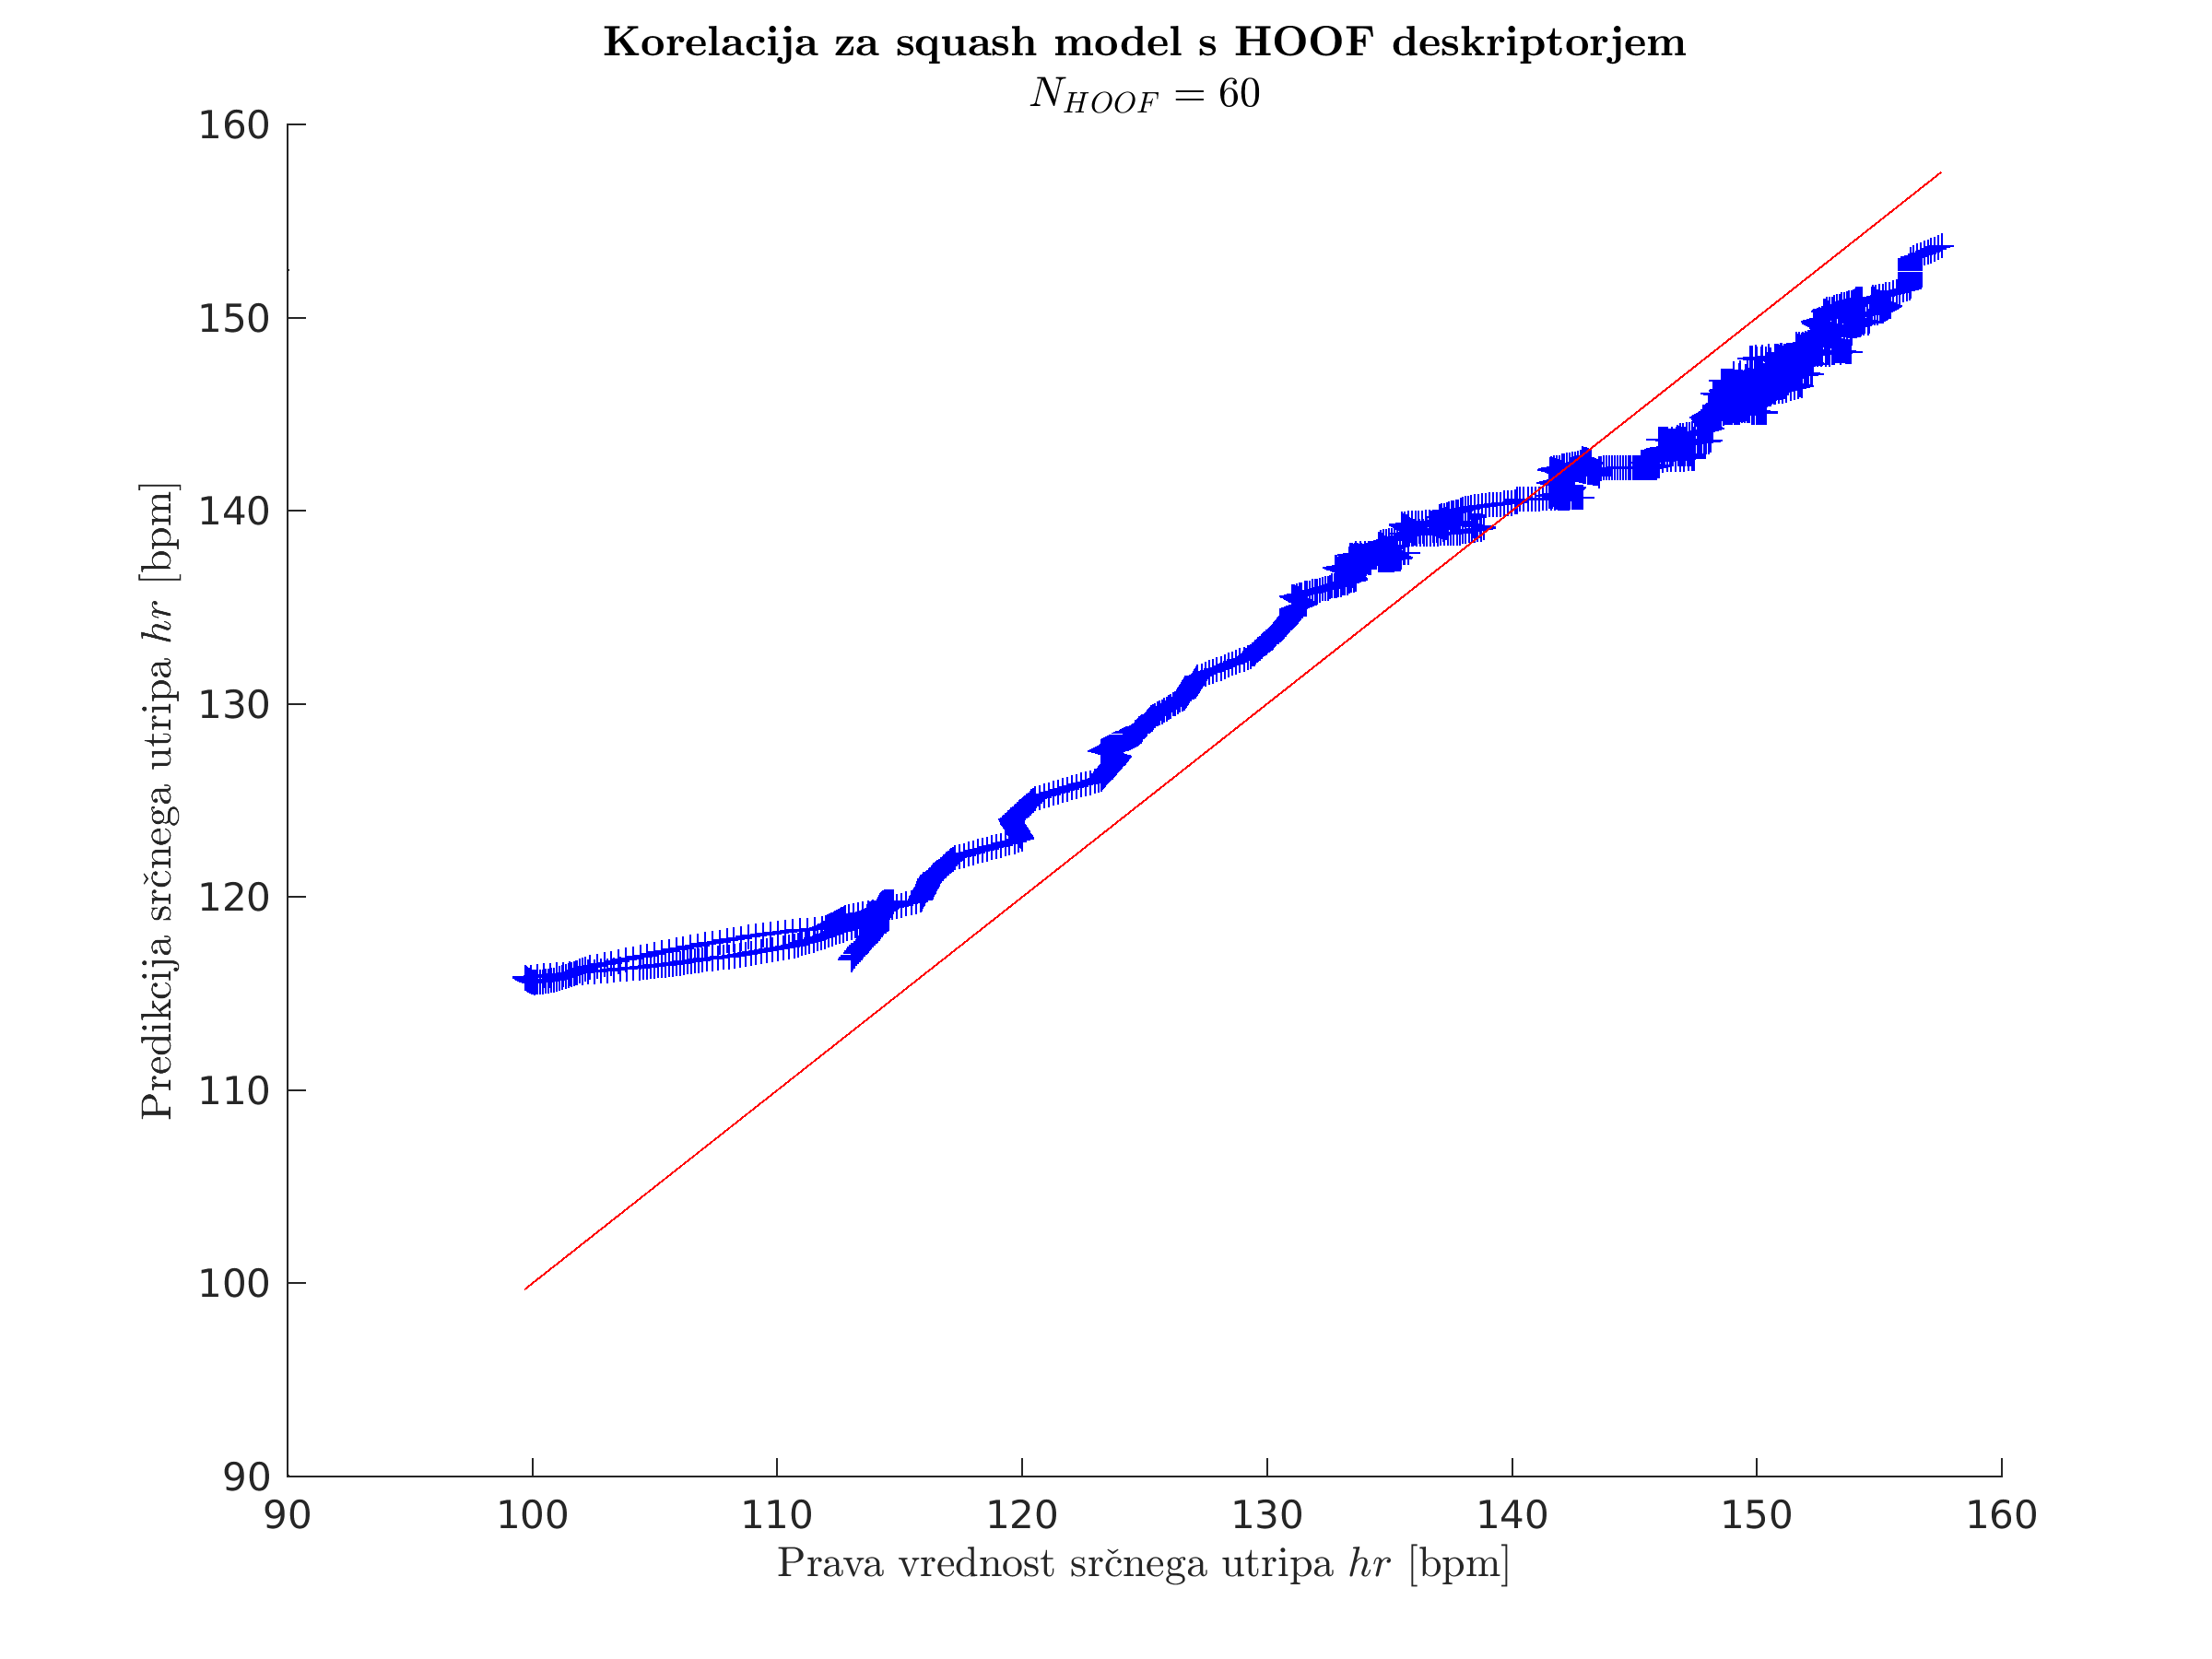
\includegraphics[width=\columnwidth]{./Slike/corr-hoof.png}
      \caption{Korelacija $N_{HOOF}=60$.}
      \label{fig:izbira-hoof}
    \end{subfigure}
    ~
    \begin{subfigure}[t]{0.45\columnwidth}
      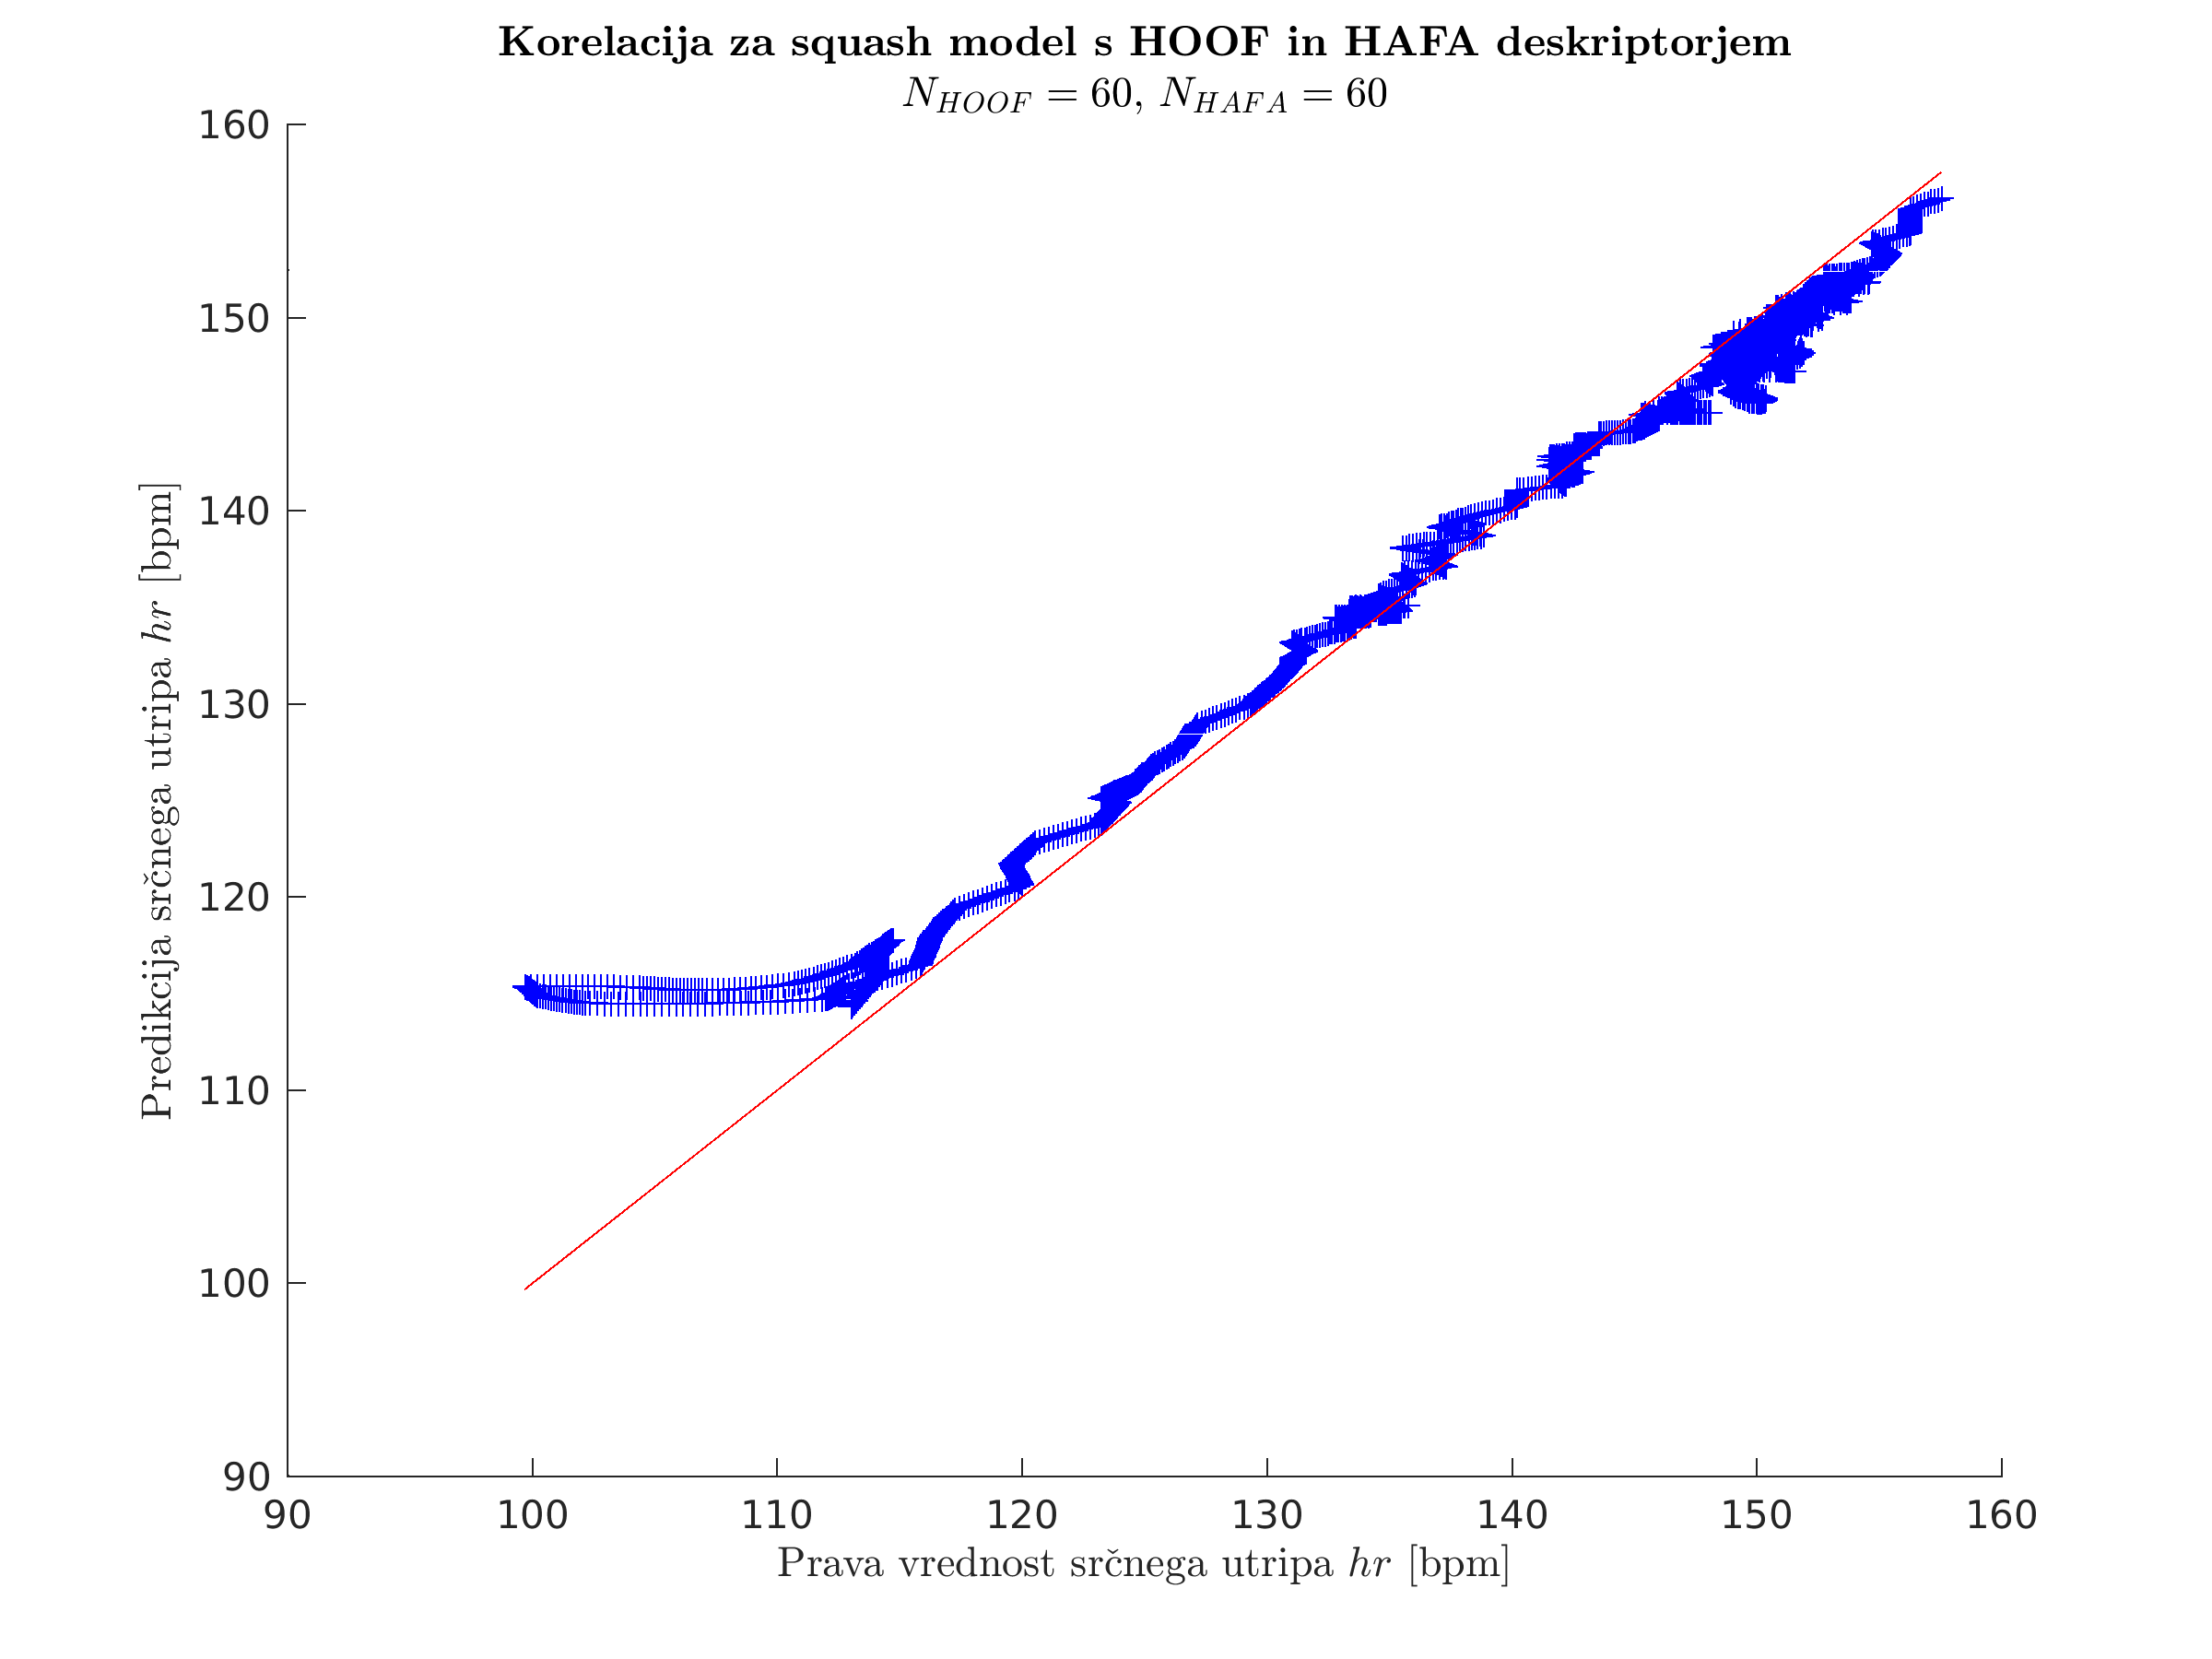
\includegraphics[width=\columnwidth]{./Slike/corr-hoof-hafa.png}
      \caption{Korelacija $N_{HOOF}=60$,\\$N_{HAFA}=60$.}
      \label{fig:izbira-hoofhafa}
    \end{subfigure}
    \caption[Primerjava modelov s HOOF in HOOF-HAFA deskriptorji]{Primerjava grafov korelacij modelov z različnimi deskriptorji. Model \subref{fig:izbira-hoof}) smo naučili s HOOF deskriptorjem. Model \subref{fig:izbira-hoofhafa}) smo naučili s HOOF in HAFA deskriptorjem. Posamezen vzorec je tako vseboval $120$ značilk. Pri primerjavi korelacije lahko opazimo vidno razliko. Model \subref{fig:izbira-hoofhafa}) dokazuje, da je razširjeni deskriptor boljši.}
    \label{fig:izbira}
\end{figure}





\subsubsection{Regresija \texorpdfstring{$\nu$}{nu}-RBF}





\subsection{Optični tok}
Na podlagi opisanih lastnosti metod optičnega toka v poglavju \ref{sec:metode-of} smo se odločili, da bomo v tem delu uporabili diferencialno metodo. Kljub višji računski zahtevnosti, ki ob današnji tehnologiji ne predstavlja več takega problema, smo želeli računati gost optični tok. Z gostim optičnim tokom tako dobimo natačno aproksimacijo polja gibanja za celotno telo. Prav tako nimamo problemov pri estimaciji energijske porabe za hitre gibe, kot bi bilo to v primeru uporabe ujemlanih metod. Ker je glavni namen uporaba in ne implementacija diferencialne metode, smo se osredotočili na Farneb{\"a}ck algoritem, ki je dostopen v knjižnici OpenCV.


\subsection{Prostorski tok}
Ker smo v našem delu za računanje prostorskega toka uporabili Kinect senzorje, smo potrebovali metodo, ki temelji na RGB-D podatkih. Ker je glavni namen uporaba in ne implementacija algoritma prostorskega toka, smo se osredotočili na PD-Flow algoritem, ki je javno dostopen \cite{jaimez2015primal}. Algoritem je podrobneje opisan v poglavju \ref{sec:pd-flow}.





\subsection{Sledilniki}
\subsubsection{Način izbire sledilnikov}\label{sec:pogoji-sledilnikov}
Pri izbiri sledilnikov smo se osredotočili na pogoje, ki jim morajo sledilniki v največji meri zadostiti.

\paragraph{Način sledenja.} Sledilnik mora dobro slediti osebam, ostali objekti niso pomembni. Sledenje mora biti zanesljivo, saj je od njega odvisna merilna napaka. Pri tem moramo upoštevati delovanje tudi v primerih, kadar tarča izgine iz slike. Sledenje mora delovati čimdaljši čas tako, da ne potrebujemo ponovne inicializacije. Inicializacijo sledilnika moramo opraviti samo na prvi sliki zaporedja, kar pomeni, da mora sledilnik vsebovati indirektno učenje (angl. offline training).

\paragraph{Implementacija.} Zaradi uporabe sledilnika v merilnem instrumentu, mora ta delovati v realnem času oziroma čim hitreje. Ker namen tega dela ni implementacija sledilnika, mora biti ta implementiran v prosto dostopni izvorni kodi. 


\subsection{Sledilnik za optični tok}
Na podlagi že prej opisanih pogojev, smo za merilno metodo z optičnim tokom našli sledilnik TLD avtorja Kalal et. al \cite{kalal2012tracking}. Prosto dostopne so tri implementacije sledilnika in sicer v knjižnici ccv (CCV-TLD), v knjižnici OpenCV (OPENCV-TLD) in c++ izvorna koda (NEBEHAY-TLD). Implementaciji iz knjižnic ccv in OpenCV se nekoliko razlikujeta od izvirnega dela \cite{kalal2012tracking}, NEBEHAY-TLD pa je samo prepis matlabove izvorne kode. Ker ni nobena implementacija zadovoljivo delovala na testnih squash posnetkih, smo poskusili še sledilnikom KCF \cite{danelljan2014adaptive} in CORR \cite{danelljan2014accurate}. KCF je implementiran v knjižnici OpenCV, CORR pa v knjižnici Dlib \cite{king2009dlib}. 




\subsubsection{Testiranje sledilnikov}
Sledilnike smo testirali na sekvencah slik \textit{handball1} in \textit{handball2} podatkovne baze VOT2016 \cite{kristan2016visual}. Sledila je še hitra vizualna ocena delovanja na kratkih izsekih video posnetka \cite{squashtv2014squash}.

Pri testiranju sekvenc slik podatkovne baze VOT2016 smo poenostavili rotirajoča referenčna področja detekcij na nerotirajoča področja. Pri tem smo za zgornji levi kot $T_0(x,y)$ in spodnji desni kot $T_1(x,y)$ uporabili enačbo \eqref{eq:vot-bb}, kjer so $\left( x_i, y_i\right), \forall i=1,\ldots,4$ ogljišča rotirajočega referenčnega področja. 

\begin{equation}
\begin{aligned}
	T_0(x,y) &= \left( \min_{i = 1,\ldots,4}\left\{x_i \right\}, 
    \min_{i=1,\ldots,4}\{y_i \} \right) \\
    T_1(x,y) &= \left( \max_{i = 1,\ldots,4}\left\{x_i \right\}, 
    \max_{i=1,\ldots,4}\{y_i \} \right)
\end{aligned}
\label{eq:vot-bb}
\end{equation}

Ker je za naš sledilnik najbolj pomembno zanesljivo delovanje, smo izbrali mero prekrivanja področja.


Video posnetek \cite{squashtv2014squash} smo za potrebe vizualne ocene delovanja na squash posnetkih razdelili na več kratkih izsekov. Pri tem smo uporabili le hrbtne posnetke mirujoče kamere. 

Rezultati testiranja so prikazani v tabeli \ref{tab:region-overlap}. Za izbrane sledilnike smo določili povprečje prekrivanja področja za posamezen posnetek. V tretjem stolpcu je predstavljeno povprečje prekrivanja glede na oba posnetka. Najboljši rezultati so odebeljeni. Po tabeli \ref{tab:region-overlap} se za posnetek \textit{handball1} najbolje izkaže CORR sledilnik. Za posnetek \textit{handball2} smo dobili najboljše rezultate pri sledilniku OPENCV-TLD. V povprečju se najbolje izkaže sledilnik CORR.




\begin{table}[htb]
	\centering
    \begin{tabular}{l S[table-format=1.3] S[table-format=1.3] S[table-format=1.3]}
    \toprule
    \textbf{Sledilnik} & \thead{$\mathbf{\Phi(\mathrm{handball1})}$} & \thead{$\mathbf{\Phi(\mathrm{handball2})}$} & \thead{$\mathbf{\overline{\Phi}}$}  \\
    \midrule%nSV
    NEBEHAY-TLD & 0.035 & 0.130 & 0.083 \\
    CCV-TLD & 0.117 & 0 & 0.117 \\
    OPENCV-TLD & 0.002 & \boldentry{1.3}{0.178} & 0.09 \\
    CORR & \boldentry{1.3}{0.214} & 0.160 & \boldentry{1.3}{0.187} \\
    \textbf{KCF} & {0.161} & {0.166} & {0.164} \\
    \bottomrule
    \end{tabular}
    \caption[Povprečje prekrivanja področja za posamezen sledilnik]{Povprečje prekrivanja področja za posamezen sledilnik in posnetek. V tretjem stolpcu je predstavljeno povprečje prekrivanja glede na oba posnetka. Najboljši rezultati so odebeljeni. Po tabeli \ref{tab:region-overlap} se za posnetek \textit{handball1} najbolje izkaže CORR sledilnik. Za posnetek \textit{handball2} smo dobili najboljše rezultate pri sledilniku OPENCV-TLD. V povprečju se najbolje izkaže sledilnik CORR.}
    \label{tab:region-overlap}
\end{table}


Na sliki \ref{fig:tracker-visual} lahko vidimo primer delovanja sledilnikov za oba posnetka. Referenčni igralec, ki mu morajo slediti ima rumeno majico. Za posnetek \textit{handball1} je predstavljena 15. slika, za posnetek \textit{handball2} pa 111. slika. Rezultati v tabeli \ref{tab:region-overlap} se skladajo z opažanji na sliki \ref{fig:tracker-visual}.

\begin{figure}[htb]
\centering

	\begin{subfigure}[t]{0.45\columnwidth}
      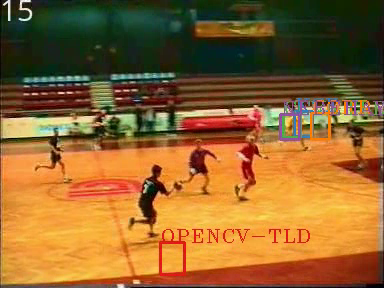
\includegraphics[width=\columnwidth]{./Slike/handball1-example.png}
      \caption{15. slika posnetka \textit{handball1}.}
      \label{fig:handball1}
    \end{subfigure}
    ~
    \begin{subfigure}[t]{0.45\columnwidth}
      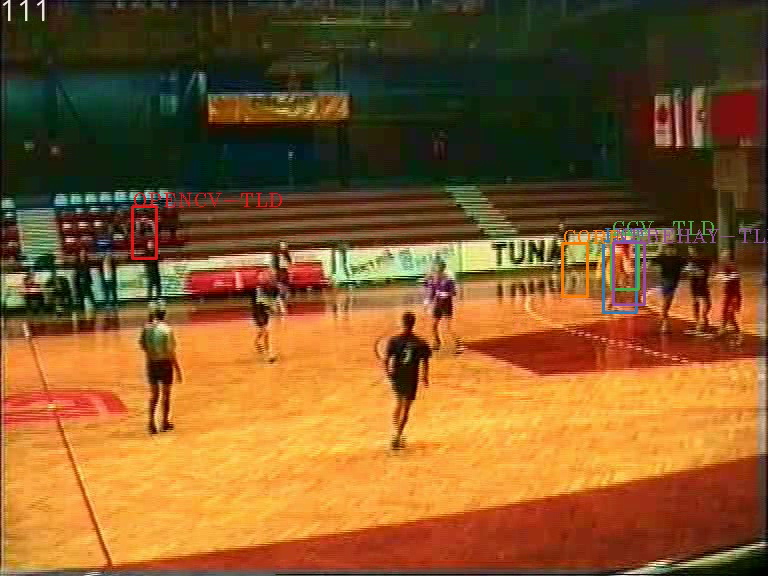
\includegraphics[width=\columnwidth]{./Slike/handball2-example.png}
      \caption{111. slika posnetka \textit{handball2}.}
      \label{fig:handball2}
    \end{subfigure}  
\caption[Primer delovanja sledilnikov za \textit{handball} posnetke]{Primer delovanja sledilnikov za \textit{handball} posnetke. Referenčni igralec, ki mu morajo slediti ima rumeno majico. }
\label{fig:tracker-visual}
\end{figure}




Čeprav smo z mero določili, da se je najbolje izkazal sledilnik CORR, se je pri hitri vizualni oceni sledenja na izsekih posnetka \cite{squashtv2014squash} izkazalo, da najbolje deluje sledilnik KCF. Primer boljšega delovanja KCF sledilnika je slika \ref{fig:squash-tracker-visual}, kjer sledimo modremu igralcu. Na isti sliki posnetka je KCF algoritem našel modrega igralca, medtem ko ga je CORR algoritem zamenjal z drugim igralcem. 



\begin{figure}[htb]
\centering

	\begin{subfigure}[t]{0.45\columnwidth}
      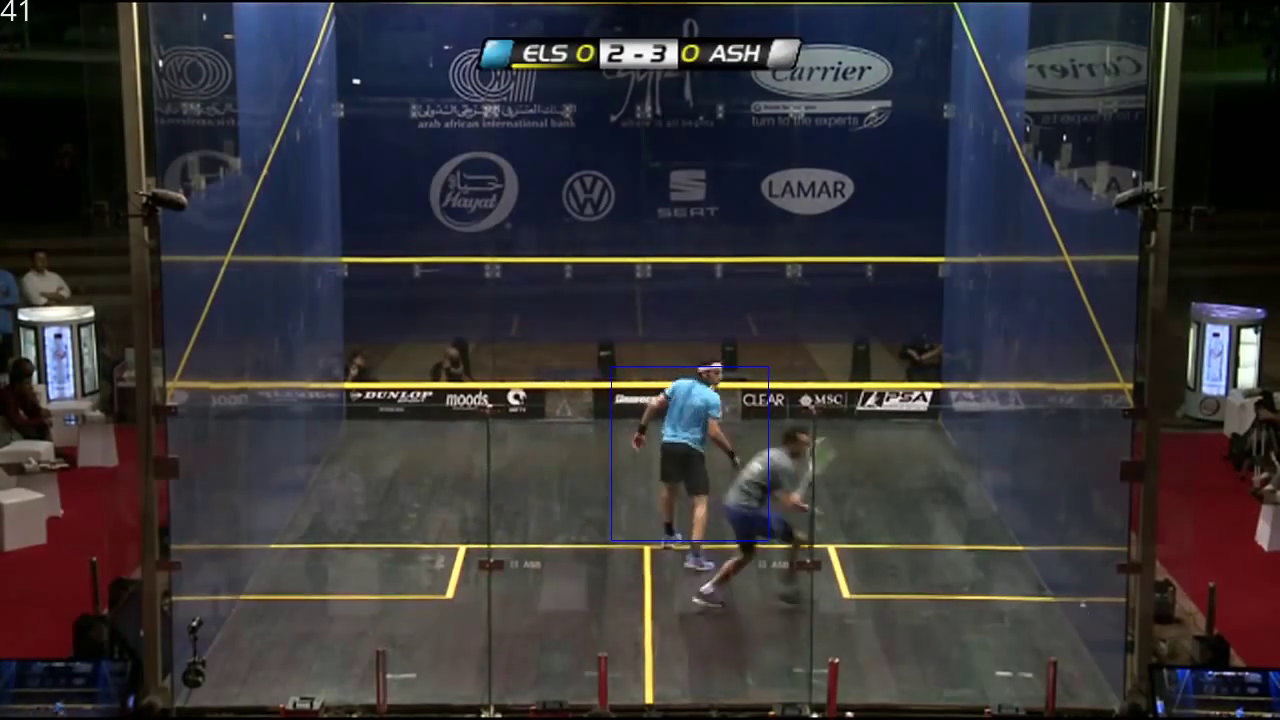
\includegraphics[width=\columnwidth]{./Slike/squash-1-kcf-example.png}
      \caption{41. slika posnetka \cite{squashtv2014squash} s KCF sledilnikom.}
      \label{fig:squash-1-kcf}
    \end{subfigure}
    ~
    \begin{subfigure}[t]{0.45\columnwidth}
      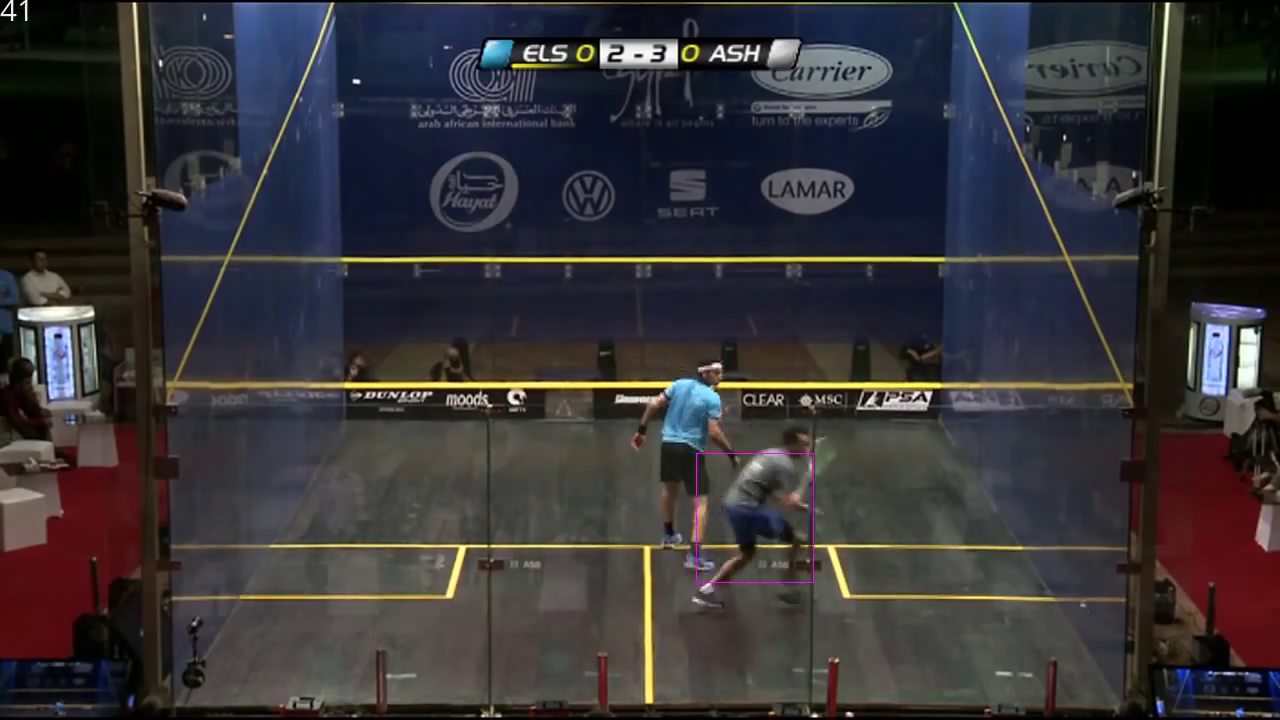
\includegraphics[width=\columnwidth]{./Slike/squash-1-corr-example.png}
      \caption{41. slika posnetka \cite{squashtv2014squash} s CORR sledilnikom.}
      \label{fig:squash-1-corr}
    \end{subfigure}  
\caption[Primer delovanja sledilnikov za squash posnetek]{Primer delovanja sledilnikov za squash posnetek. Gre za identični sliki posnetka, pri čemer smo na sliki \ref{fig:squash-1-kcf} uporabili KCF algoritem, na sliki \ref{fig:squash-1-corr} pa CORR algoritem. Sledilnika sta morala slediti igralcu z modro majico.}
\label{fig:squash-tracker-visual}
\end{figure}


Boljše delovanje KCF je razumljivo, saj prvi testi temeljijo na posnetkih rokometa, drugi pa na squashu, kjer gre za bistveno drugačno igro. Če pogledamo tabelo \ref{tab:region-overlap} ima KCF drugo najboljše povprečje, prav tako pa so si rezultati posameznih posnetkov zelo podobni. 


\subsubsection{Sledilnik za prostorski tok}
Na podlagi pogojev iz poglavja \ref{sec:pogoji-sledilnikov} smo za merilno metodo s prostorskim tokom našli le DS-KCF sledilnik avtorja Hannuna et. al \cite{hannuna2016ds}. 





\subsection{Kalmanov filter}
Za prostor stanj smo izbrali stanje hitrosti $v$ in pospeška $a$ \eqref{eq:stanje}. 

\begin{equation}
\vec{x}(k) = \begin{bmatrix}
					v(k) & a(k)
				\end{bmatrix}^\top 
                \label{eq:stanje}
\end{equation}

Matrika prehajanja stanj je določena z enačbo \eqref{eq:a}.

\begin{equation}
\vec{A} = \begin{bmatrix}
				1 & 1 \\
                0 & 1
			\end{bmatrix} 
            \label{eq:a}
\end{equation}

Za matriko vhodnih stanj $G$ smo izbrali \eqref{eq:g}, s katero modeliramo neznane vhodne parametre hitrosti $v_n$ in pospeška $a_n$ v vektorju $u$ \eqref{eq:u}. 

\begin{equation}
\vec{G} = \begin{bmatrix}
				1 & 0
			\end{bmatrix}^\top 
            \label{eq:g}
\end{equation}

\begin{equation}
\vec{u}(k) = \begin{bmatrix}
					v_{n}(k) & a_n(k)
				\end{bmatrix}^\top 
                \label{eq:u}
\end{equation}


Merilna matrika je predstavljena z enačbo \eqref{eq:h}
\begin{equation}
\vec{H} = \begin{bmatrix}
				1 & 0
			\end{bmatrix}^\top 
            \label{eq:h}
\end{equation}

Za začetno hitrost in pospešek smo izbrali vrednost $0$, ker se naši testi večinoma začnejo v mirovanju. 

Variance šuma modela gibanja, merilnega modela in konvaričane matrike stanja smo določili z uporabo mrežnega iskanja, ki je opisan v poglavju \ref{sec:optimizacija-svm-parametrov}. Pri tem smo uporabili labele učnih vzorcev vseh testov 1. sklopa eksperimentov za referenco, njihove pošumljene ocene pa za meritev. Varianca šuma merilnega modela je tako znašala $\sigma_\vec{z}^2 = 0.04$, varianca šuma modela gibanja pa $\sigma_\vec{x}^2 = 456.13$. Za kovariančno matriko predikcije smo uporabili varianco $\sigma_\vec{P}^2 = 456.13$. Kovariančno matriko modela gibanja smo določili po enačbi \eqref{eq:Q}, kovariančna matrika merilnega modela je bila določena z enačbo \eqref{eq:R} in začetna vrednost kovariančne matrike stanja z \eqref{eq:P}.

\begin{equation}
\vec{Q} = \vec{G} \vec{G}^\top \sigma_\vec{x}^2
\label{eq:Q}
\end{equation}

\begin{equation}
\vec{R} = \sigma_\vec{z}^2
\label{eq:R}
\end{equation}

\begin{equation}
\vec{P}(0) = \begin{bmatrix}
1 & 0 \\
0 & 1
\end{bmatrix} \sigma_\vec{P}^2
\label{eq:P}
\end{equation}





\subsubsection{Optimizacija Gaussovega jedra}
Pri optimizaciji Gaussovega jedra smo določili optimalni standardni odklon $\sigma$ z uporabo dveh metrik, in sicer: koren srednje kvadratične napake (RMSE) in razmerje med signalom in šumom (SNR). Pri RMSE metriki smo določili napako med učnimi vzorci in njihovo predikcijo. Pri SNR metriki smo za signal uporabili referenčne učne vzorce. Za šum smo uporabili rezidualni ali preostali šum. Tega smo dobili z odštevanjem filtriranih vzorcev od referenčnih. SNR metrika tako določa uspešnost izločevanja šuma, RMSE metrika pa pravilnost določevanja kateri podatki spadajo v signal in kateri v šum.


Teste smo izvajali na vseh eksperimentih 1. sklopa, pri čemer smo uporabili $\nu$-RBF jedro s \SI{50}{\%} podpornih vektorjev. Za filtriranje pri mrežnem iskanju smo izbrali najmanjši filter s $\sigma = 1$. Testirali smo naslednje standardne odklone Gaussovega filtra: $1, 3, 5, 11, 21, 31$ in $51$. 

Rezultati povrprečnih vrednosti uporabljenih metrik so vidni v tabeli \ref{tab:gauss}. Za pravilno razlago rezultatov, moramo upoštevati tudi grafe metrik posameznih eksperimentov, ki so prikazani na slikah \ref{fig:sigma1-5}, \ref{fig:sigma-rmse5-21} in \ref{fig:sigma21-51}. 



\begin{table}[htb]
	\centering
    \begin{tabular}{S[table-format=2.0] S[table-format=2.3] S[table-format=2.3]}
    \toprule
    \thead{$\mathbf{\sigma}$} & \thead{RMSE} & \thead{SNR [dB]}  \\
    \midrule%nSV
    1 & \boldentry{2.3}{8.614} & 24.278 \\
    3 & 11.236 & 25.470 \\
    \boldentry{2.0}{5} & 11.596 & 25.746 \\
    11 & 11.783 & 25.746 \\
    21 & 11.842 & 25.975 \\
    31 & 11.871 & 26.194 \\
    51 & 11.907 & \boldentry{2.3}{26.306} \\
    \bottomrule
    \end{tabular}
    \caption[Povprečne vrednosti RMSE in SNR metrik pri optimizaciji parametra $\sigma$ Gaussovega filtra]{Povprečne vrednosti RMSE in SNR metrik pri optimizaciji parametra $\sigma$ Gaussovega filtra. Najmanjši standardni odklon ima najmanjšo napako, vendar je tudi filtriranje majhno. Pri $\sigma=3$ in $\sigma=5$ so še opazne razlike pri filriranju. Za višje vrednosti ni več opazne razlike, vendar pa se napaka povečuje. $\sigma=5$ je tako optimalna vrednosti parametra.}
    \label{tab:gauss}
\end{table}

Najmanjšo napako dobimo, če uporabimo $\sigma=1$, vendar pa imamo pri tem najmanjše filtriranje, zato so rezultati še vedno lahko zelo šumni. Z višanjem parametra filtra, se napaka po metriki RMSE povečuje, vendar ima večji vpliv razmerje SNR, saj je predstavljeno v logaritemski skali. 

\begin{figure}[htb]
\centering
\begin{subfigure}[t]{0.45\columnwidth}
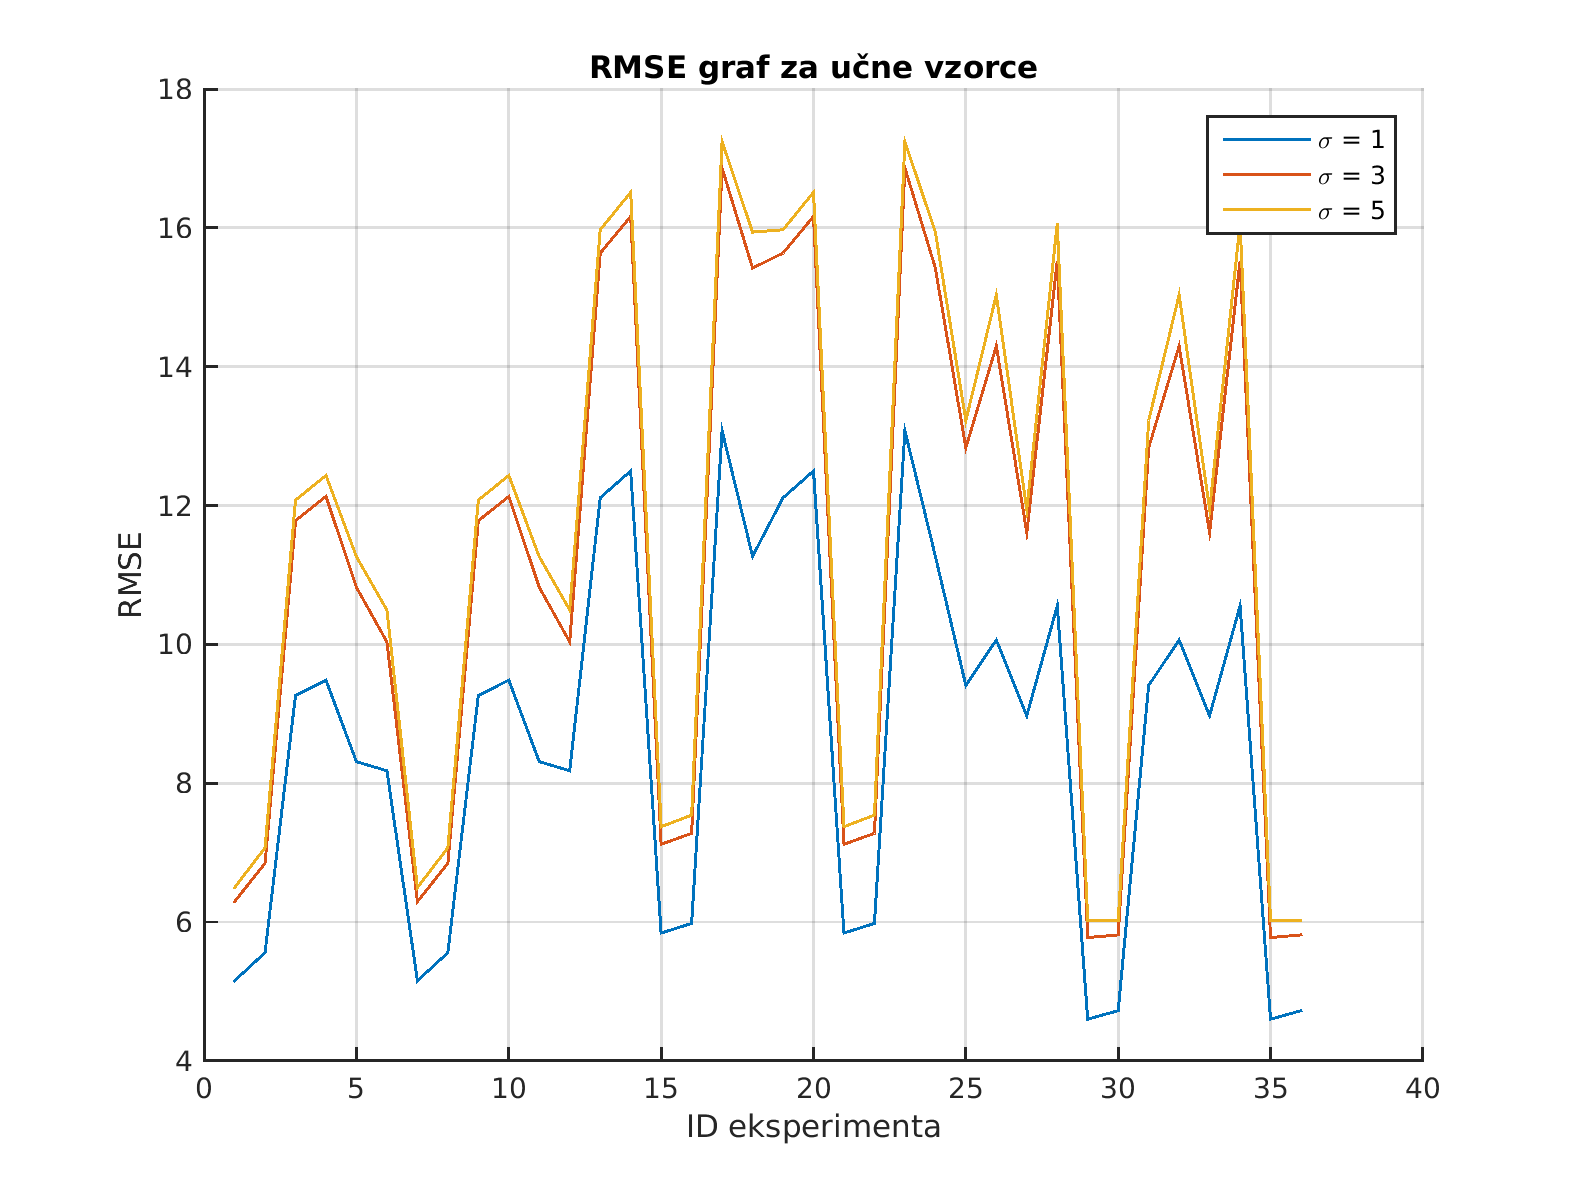
\includegraphics[width=\columnwidth]{./Slike/sigma-rmse1-5.png}
\caption{Graf RMSE  učnih vzorcev }
\label{fig:sigma-rmse1-5}
\end{subfigure}
~
\begin{subfigure}[t]{0.45\columnwidth}
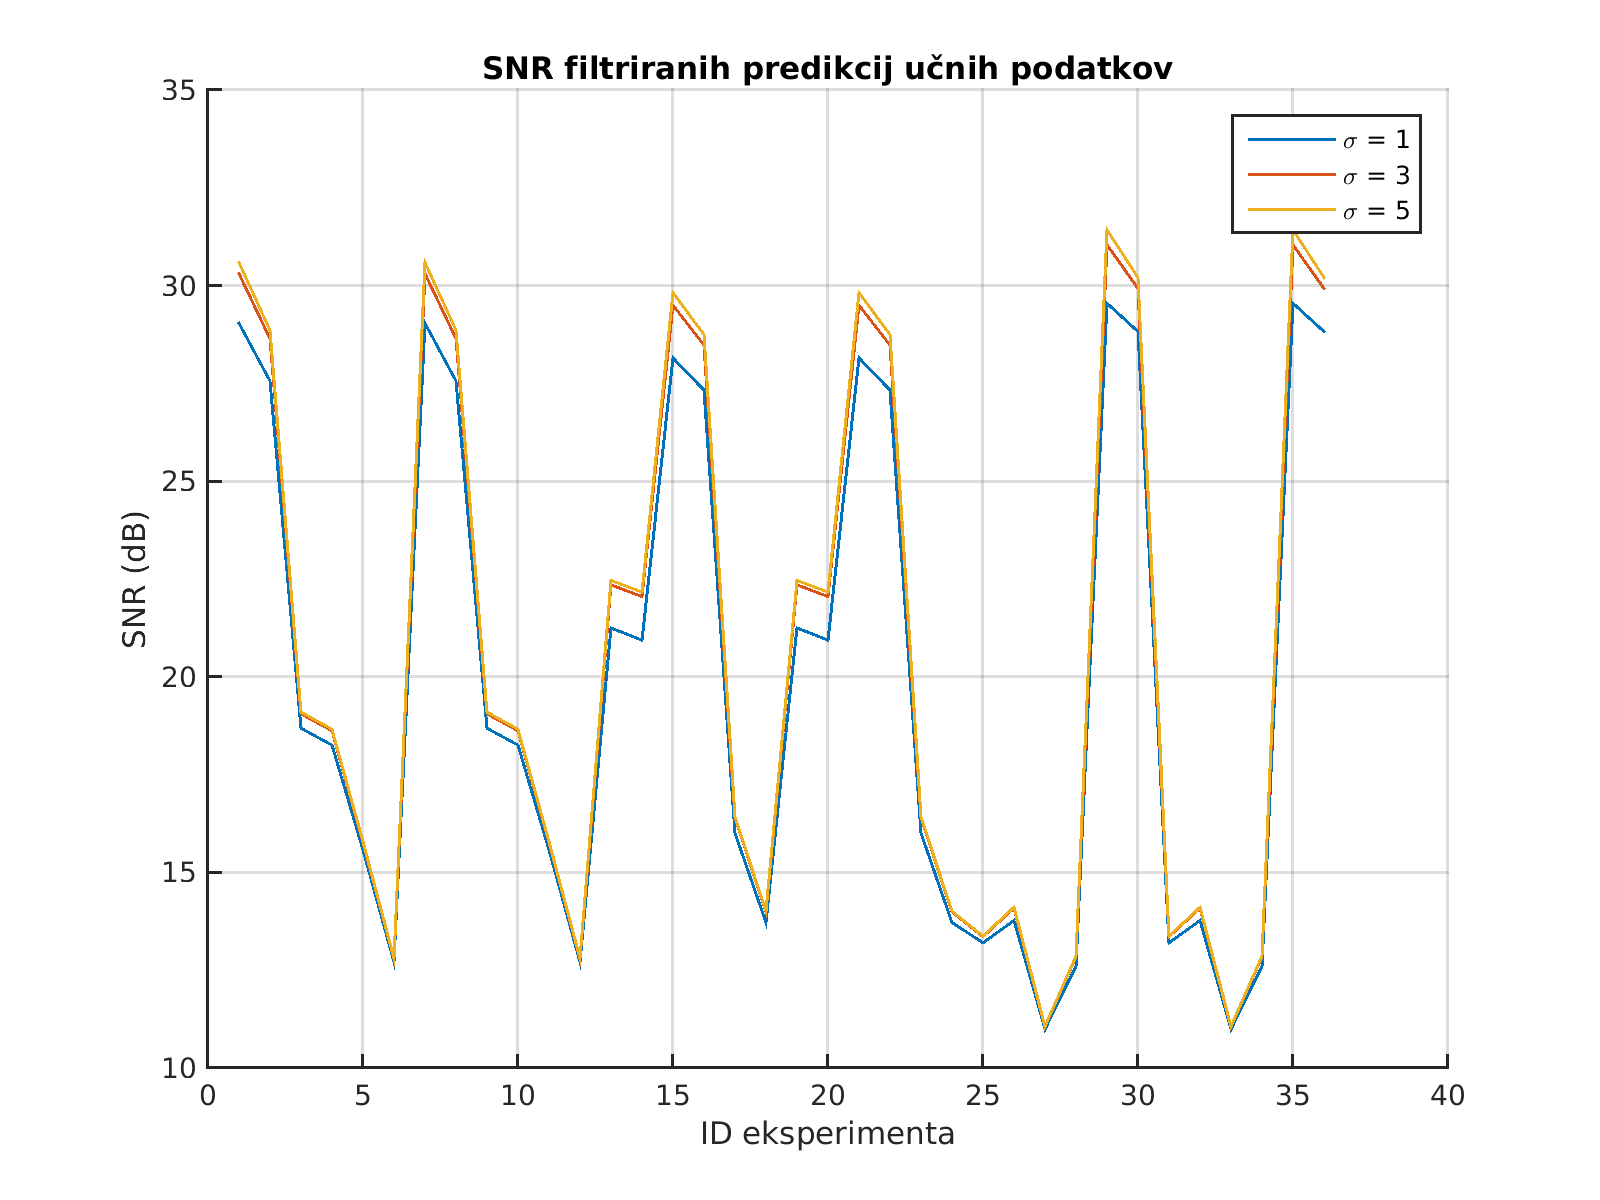
\includegraphics[width=\columnwidth]{./Slike/sigma-snr1-5.png}
\caption{Graf SNR  učnih vzorcev}
\label{fig:sigma-snr1-5}
\end{subfigure}
\caption{Grafa RMSE in SNR učnih vzorcev za \mbox{$\sigma \in [1,5]$}}
\label{fig:sigma1-5}
\end{figure}

Čeprav pri uporabi $\sigma=51$ dobimo največje filtriranje šuma, lahko na slikah grafov opazimo, da se obe metriki bistveno ne razlikujeta za vrednosti parametra na intervalu $[5,51]$. Kljub dobremu filtriranju želimo zagotoviti čim manjšo napako med referenčnim signalom in predikcijo, zato je logična izbira čim manjši standardni odklon. Ker so na sliki \ref{fig:sigma1-5} med $\sigma=3$ in $\sigma=5$ še opazne razlike, lahko zaključimo, da je $\sigma=5$ optimalna izbira parametra za naš problem. 


\begin{figure}[htb]
\centering
\begin{subfigure}[t]{0.45\columnwidth}
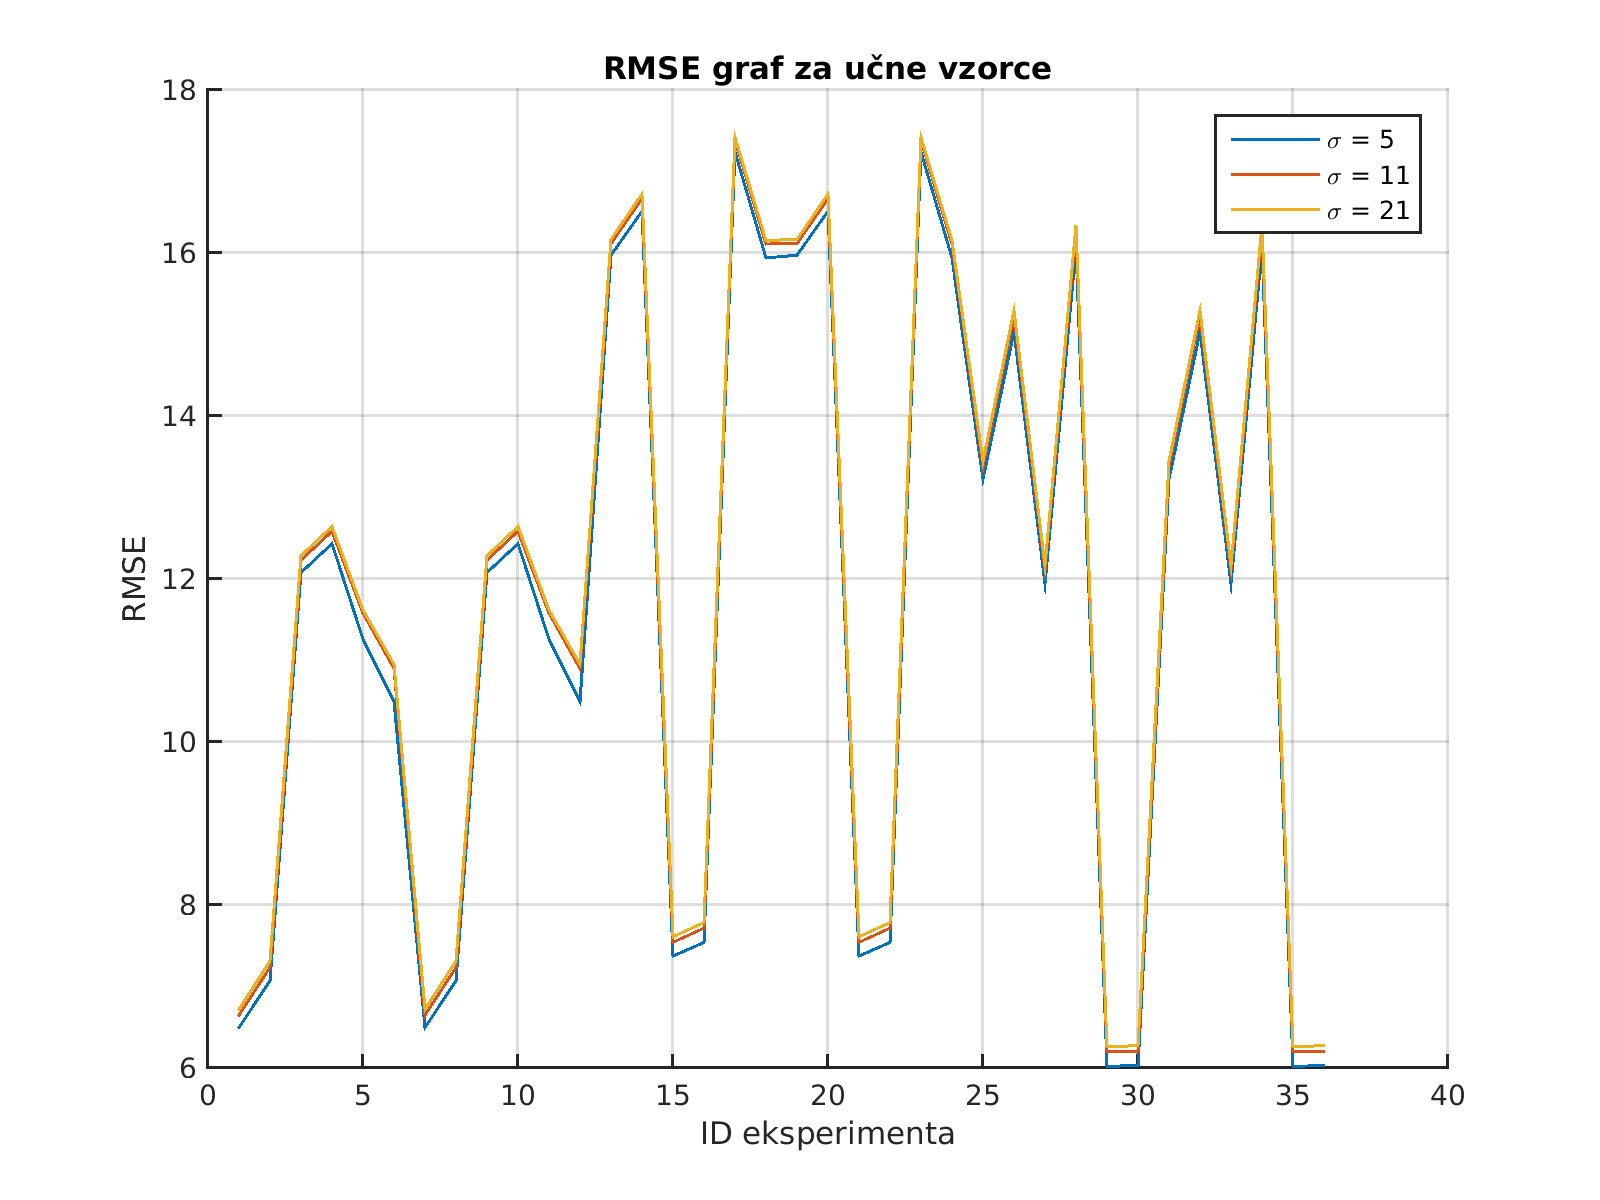
\includegraphics[width=\columnwidth]{./Slike/sigma-rmse5-21.png}
\caption{Graf RMSE  učnih vzorcev}
\label{fig:sigma-rmse5-21}
\end{subfigure}
~
\begin{subfigure}[t]{0.45\columnwidth}
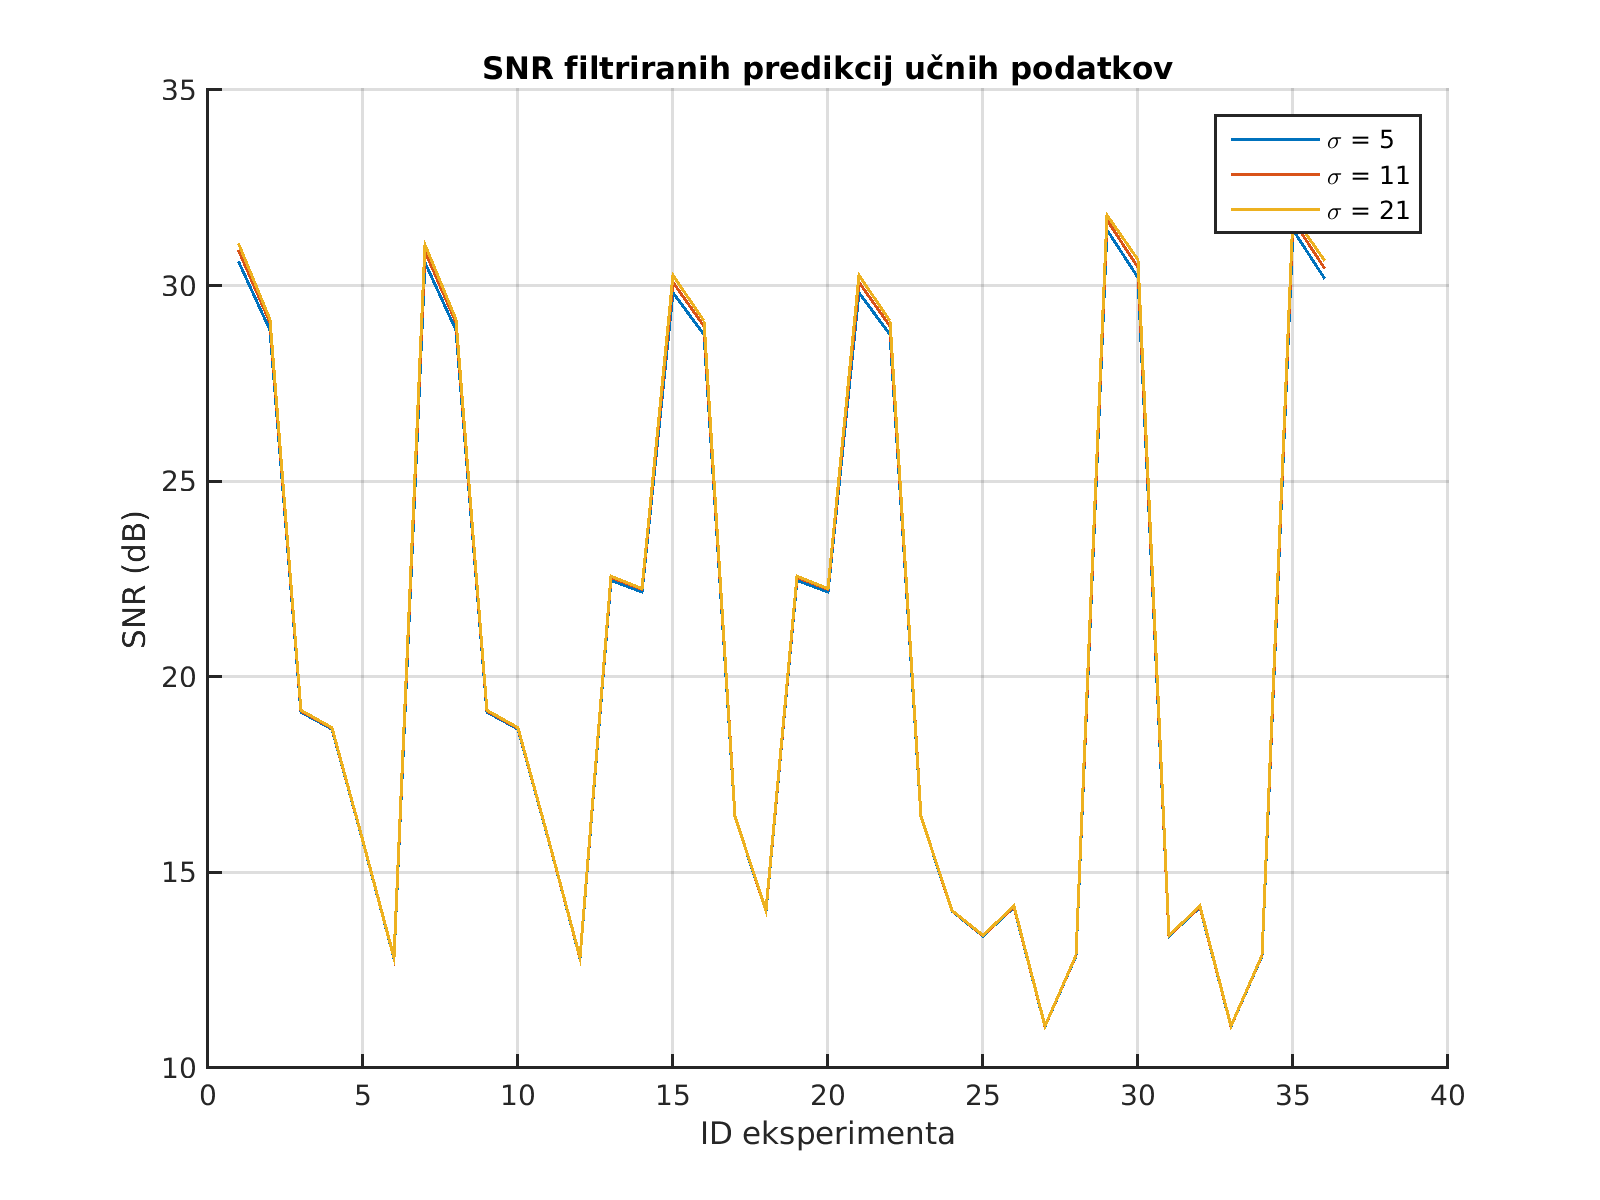
\includegraphics[width=\columnwidth]{./Slike/sigma-snr5-21.png}
\caption{Graf SNR  učnih vzorcev}
\label{fig:sigma-snr5-21}
\end{subfigure}
\caption{Grafa RMSE in SNR učnih vzorcev za \mbox{$\sigma \in [5,21]$}}
\label{fig:sigma5-21}
\end{figure}



\begin{figure}[htb]
\centering
\begin{subfigure}[t]{0.45\columnwidth}
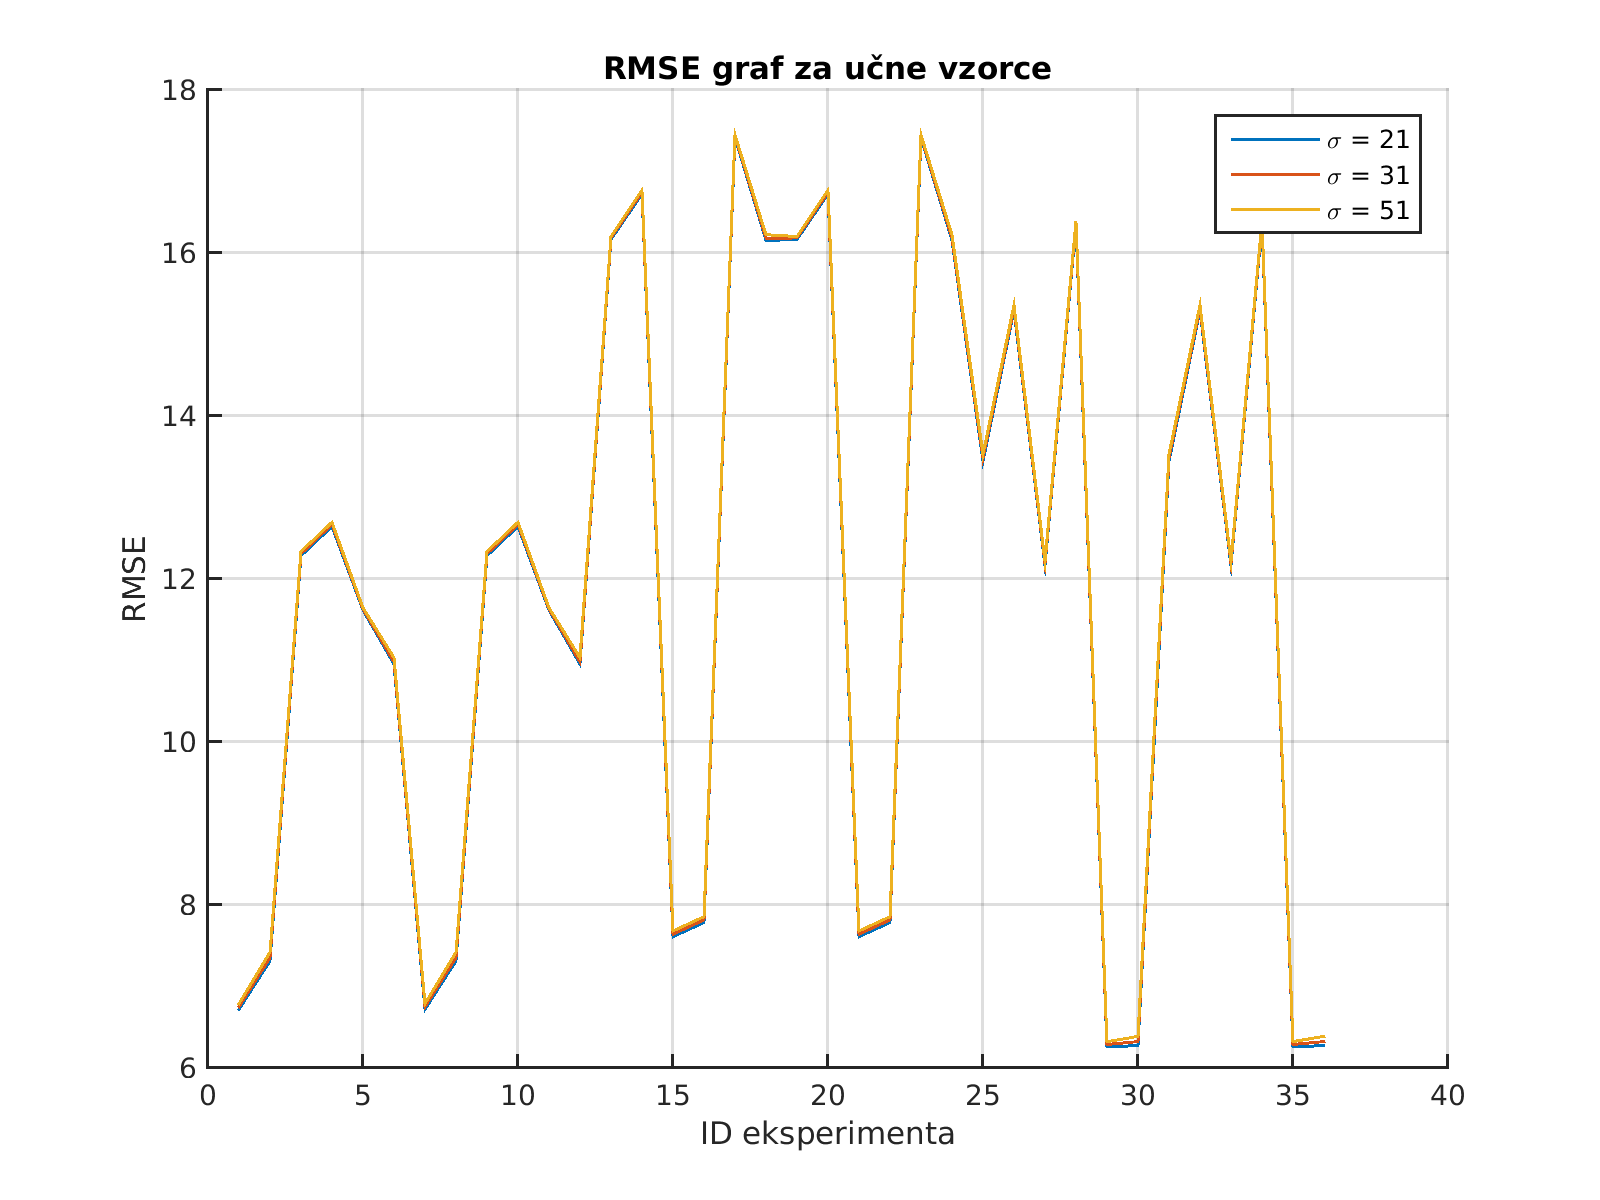
\includegraphics[width=\columnwidth]{./Slike/sigma-rmse21-51.png}
\caption{Graf RMSE učnih vzorcev}
\label{fig:sigma-rmse21-51}
\end{subfigure}
~
\begin{subfigure}[t]{0.45\columnwidth}
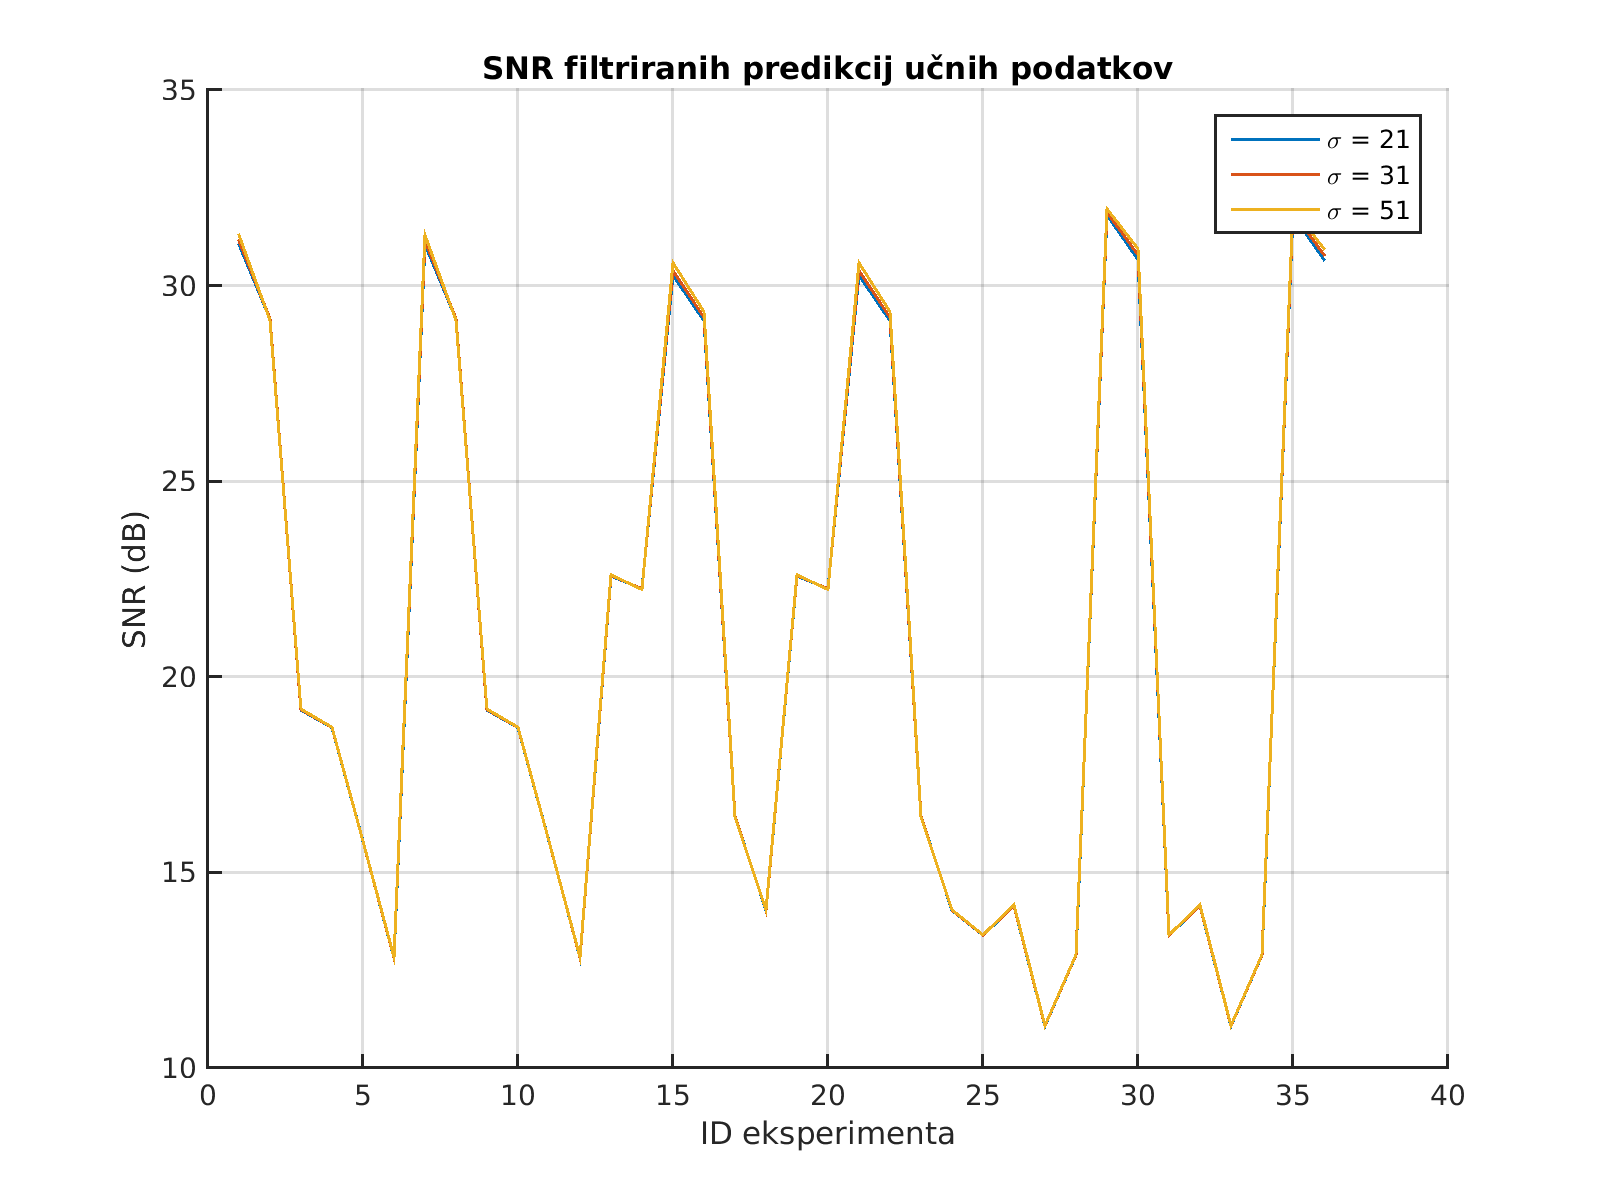
\includegraphics[width=\columnwidth]{./Slike/sigma-snr21-51.png}
\caption{Graf SNR  učnih vzorcev}
\label{fig:sigma-snr21-51}
\end{subfigure}
\caption{Grafa RMSE in SNR učnih vzorcev za \mbox{$\sigma \in [21,51]$}}
\label{fig:sigma21-51}
\end{figure}



\subsection{Implementacija Gaussovega filtra}
Gaussovo jedro smo implementirali po enačbi \eqref{eq:gauss} in ga nato še normirali. Za filtriranje podatkov smo uporabili Matlabovo funkcijo \texttt{filtfilt}, ki je primerna za hitro računanje s filtri z ničelno fazo, saj uporablja tehniko dvosmernega filtriranja.




\subsection{Projektivna transformacija preliminarnih testov}
Projektivno transformacijo smo izvedli s pomočjo matlabovih funkcij \texttt{fitgeotrans} in \texttt{imwarp}. Za vhodne točke smo izbrali robove posamezne slike zaporedja. Za izhodne točke smo izbrali vrednosti v tabeli \ref{tab:projective}, pri čemer so $h$ dolžina slike $w$ širina slike ter $x$ in $y$ slikovni koordinati.

\begin{table}[htb]
\centering
\begin{tabular}{l S[table-format=1.3] S[table-format=1.3] }
	\toprule
	\thead{Točka} & \thead{$\mathbf{x~[\times w]}$} & \thead{$\mathbf{y~[\times h]}$} \\
    \midrule
	$P_0$ & 0 & 0.25 \\
    $P_1$ & 1 & 0 \\
    $P_2$ & 0.125 & 0.75 \\
    $P_3$ & 0.875 & 0.875 \\
    \bottomrule
\end{tabular}
\caption{}
\label{tab:projective}
\end{table}

\subsection{Simulacija vibracij kamere}
Kadar uporabljamo ročne kamere, pogosto pride do tresenja. Vibracije smo simulirali z majhnimi naključnimi premiki in rotacijo posameznih slik iz video zaporedja. Vsako sliko smo transformirali z Evklidsko transformacijo. Pri tem smo translacijo omejili na \SI{4}{\%} velikosti slike. Rotacija je bila omejena na \SI{0.13}{rad}. 

Translacijo in rotacijo smo filtrirali še s Kalmanovim filtrom, tako da smo dobili bolj realistično simulacijo. Za Kalmanov filter smo uporabili enak model, kot je predstavljen v poglavju \ref{sec:kalmanov-filter}. Začetne variance filtra smo določili empirično tako, da smo dobili čimbolj realistične rezultate. Varianca šuma merilnega modela je znašala $\sigma_\vec{z}^2=1024$, variancal šuma modela gibanja pa $\sigma_\vec{x}^2=2$. Za kovariančno matriko predikcije smo uporabili varianco $\sigma_\vec{P}^2=2$.


\subsection{Združevanje slik iz dveh Kinect kamer}
Zaradi ozkega vidnega polja Kinect kamer smo za pokritje celotne širine igrišča potrebovali dve kameri. Zaporedja slik smo pred nadaljno obdelavo morali združiti v eno zaporedje glede na opazovanega igralca.

Zajem iz posameznih kamer ni bil sinhroniziran, zato smo pred združevanjem sinhronizirali posnetka tako, da smo izbrali slike iz posameznega zaporedja z najbolj podobnimi časovnimi žigi. 

\subsubsection{Združevanje z značilkami}
Časovno sinhronizirana zaporedja slik, smo najprej poskušali združiti z metodo panoramskega šivanja slik z uporabo značilk, kot je opisano v delu \cite{brown2007automatic}. Tu smo namesto SIFT značilk uporabili SURF značilke. Združevanje s značilkami se ni obneslo, zato smo to metodo opustili. Primer neuspelega poskusa je prikazan na sliki \ref{fig:zdruzevanje-znacilke}.

\begin{figure}[htb]
\centering
\begin{subfigure}[t]{0.45\columnwidth}
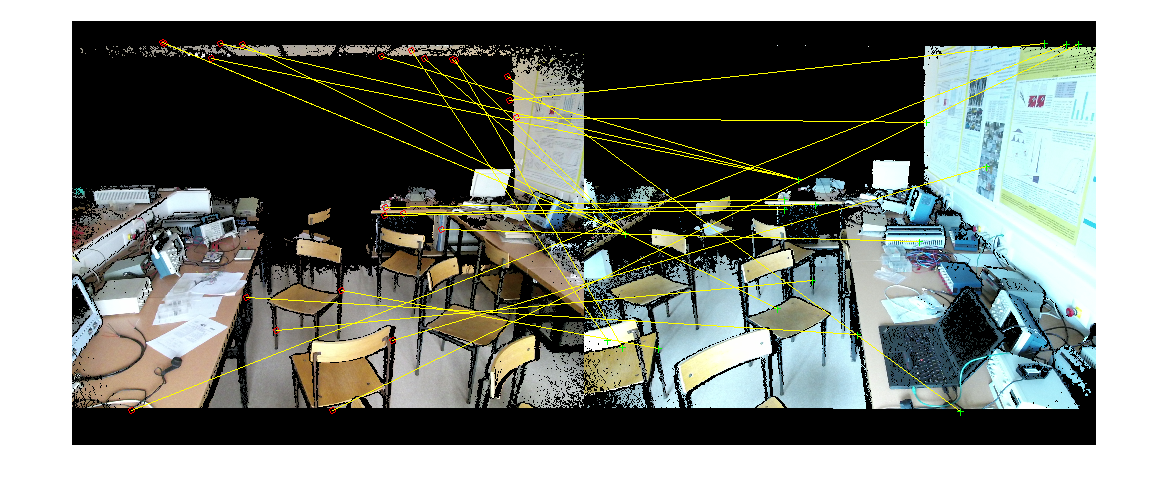
\includegraphics[width=\columnwidth]{./Slike/matched-features.png}
\caption{Ujemajoče SURF značilke}
\label{fig:zdruzevanje-surf}
\end{subfigure}
~
\begin{subfigure}[t]{0.45\columnwidth}
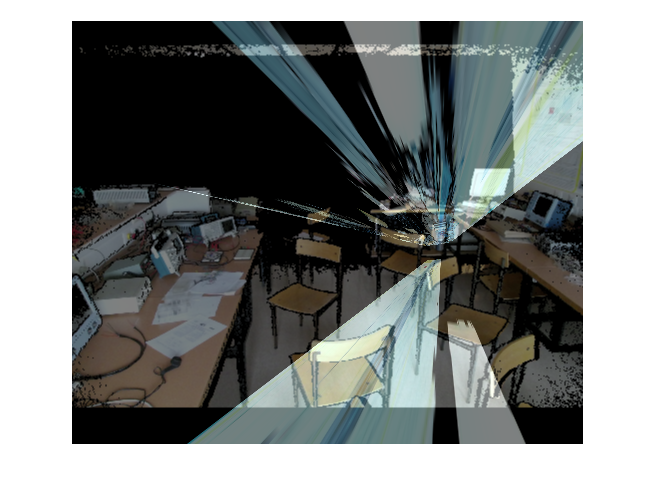
\includegraphics[width=\columnwidth]{./Slike/features-calibration-result.png}
\caption{Rezultat združevanja z značilkami}
\label{fig:zdruzevanje-result}
\end{subfigure}
\caption{Primer neuspelega poskusa združevanja slik iz dveh Kinect kamer s SURF značilkami.}
\label{fig:zdruzevanje-znacilke}
\end{figure}

\subsubsection{Združevanje s kontrolnimi točkami}
Zaporedja slik smo poskušali združiti z ročnim določevanjem kontrolnih točk. Rezultat je bil boljši od združevanja z značilkami, vendar še vedno slab, zato smo tudi to metodo opustili. Primer neuspelega poskusa je prikazan na sliki \ref{fig:zdruzevanje-cp}.

\begin{figure}[htb]
\centering
\begin{subfigure}[t]{0.45\columnwidth}
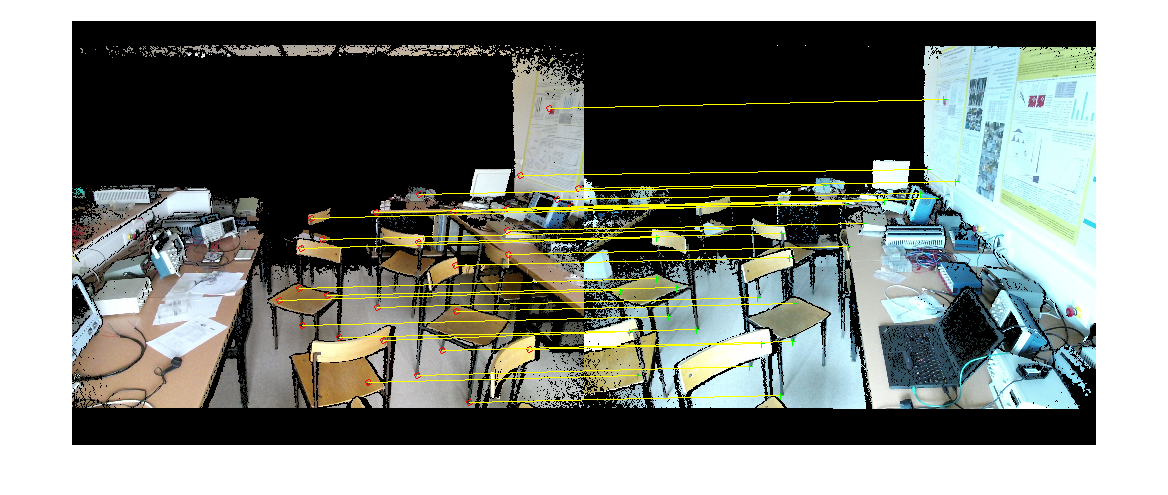
\includegraphics[width=\columnwidth]{./Slike/matched-points.png}
\caption{Ujemajoče kontrolne točke}
\label{fig:zdruzevanje-ujemajoce-cp}
\end{subfigure}
~
\begin{subfigure}[t]{0.45\columnwidth}
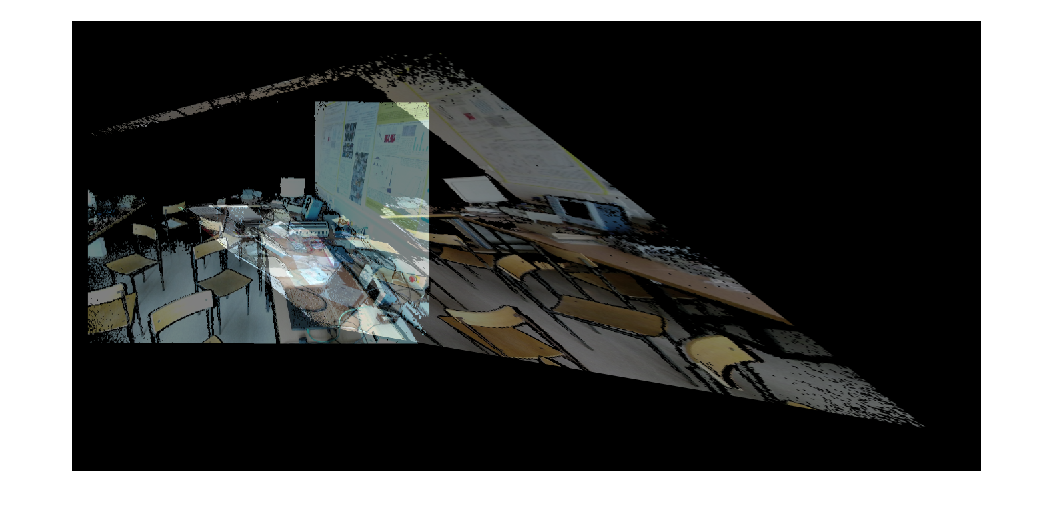
\includegraphics[width=\columnwidth]{./Slike/points-calibration-result.png}
\caption{Rezultat združevanja s kontrolnimi točkami}
\label{fig:zdruzevanje-result-cp}
\end{subfigure}
\caption{Primer neuspelega poskusa združevanja slik iz dveh Kinect kamer s kontolnimi točkami}
\label{fig:zdruzevanje-cp}
\end{figure}


\subsubsection{Prilagojeno združevanje}
Zaradi nezadovoljivih rezultatov klasičnih metod združevanja stereo slik, smo razvili metodo, ki je prilagojena za Kinect kamere. Iz kamer smo pridobili intrinzične parametre infra-redečega (IR) senzora, in sicer: slikovni koordinati goriščne razdalje $f_u$ in $f_v$ ter slikovni koordinati optičnega središča slike (ang. principal point) $c_u$ in $c_v$. Intrinsične parametre smo uporabili za določitev intrizične matrike $\vec{M}_{int}$ po enačbi \eqref{eq:intrinsic}.


Ker pravih ekstrinsičnih parametrov kamer nismo poznali, smo jih le ocenili z metodo določevanja sečišča vidnih polj obeh kamer. Sečišče je prikazano kot rdeča linija na sliki \ref{fig:zdruzevanje}. S to metodo smo določili translacijski vektor $\vec{t} = \left [ t_x~ t_y~ t_z \right]^\top$ in rotacijsko matriko $\vec{R}$ iz Eulerjevih kotov.

S sledenjem igralca z DS-KCF algoritmom, smo s pomočjo projekcijske matrike \eqref{eq:projection-matrix} določili center tarče v metričnih enotah za vsako sliko zaporedja leve in desne kamere. Kadar slikovni element ni vseboval podatkov globine, smo za center tarče izbrali najbližji slikovni element z veljavno globino.

Prva slika združenega zaporedja je bila slika kamere, kjer se igralec prvič pojavi. Nadaljne slike smo izbirali med zaporedjema kamer glede na pozicijo centra tarče. Ko je šel center tarče skozi upragovljeno mejo, ki je na sliki \ref{fig:zdruzevanje} prikazana z modro linijo smo preklopili na drugo kamero. Razdalja med pragom in sečiščem je znašala \SI{200}{mm}.


\begin{figure}[htb]
\centering
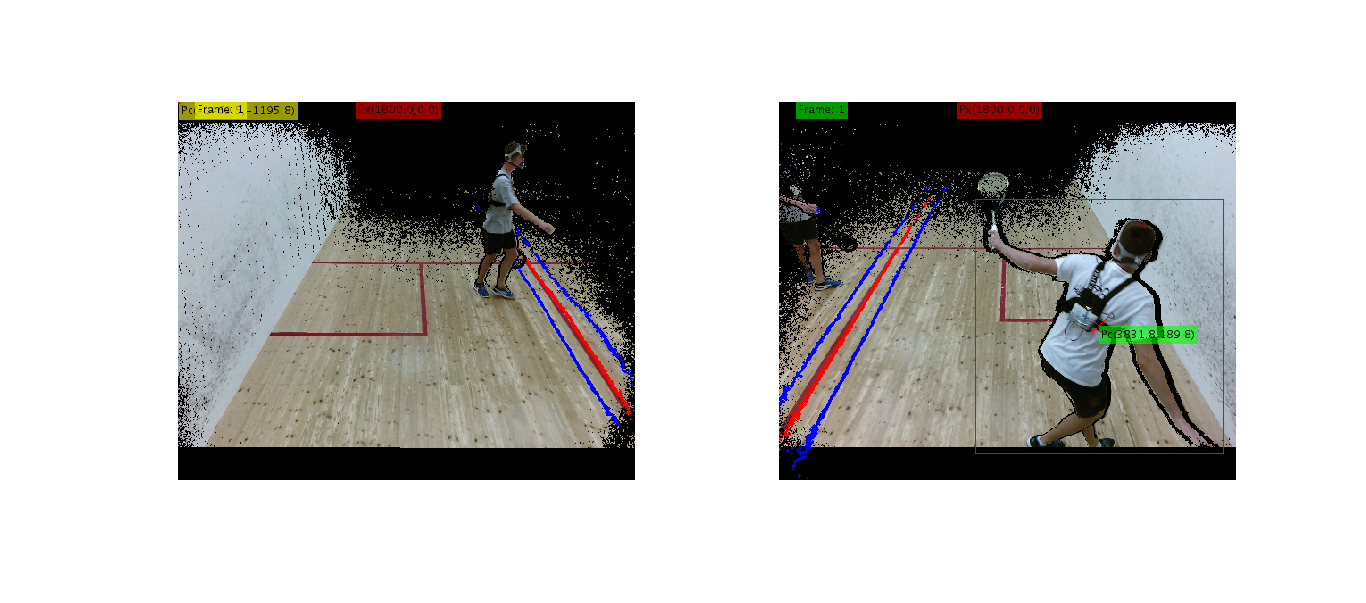
\includegraphics[width=\columnwidth]{./Slike/zdruzevanje-example.png}
\caption[Določevanje sečišča vidnih polj leve in desne Kinect kamere]{Določevanje sečišča vidnih polj leve in desne Kinect kamere. Na sliki sta prikazani prvi sliki zaporedja leve in desne Kinect kamere 1. seta 2. igre terenskega eksperimenta iz 2. faze. Označen je 4. igralec. Zelena barva koordiat središča tarče predstavlja izbrano kamero. Kamera z rumeno barvo ni izbrana. Sečišče je rdeča linija. Modri liniji sta pragova za preklop med kamerama. Ležita \SI{200}{mm} levo in desno od sečišča.}
\label{fig:zdruzevanje}
\end{figure}











\section{Eksperimenti 1. faze}

We present multiple experiments in varied environments, addressing measurement of instantaneous energy consumption, heart rate (considered the proxy for energy consumption) and breathing. In all cases, physiological parameters $eem(t)$, $hr(t)$, $breathing(t)$ were predicted from \emph{one} optical flow image via feature vector at the time $\mathbf{X}(t-lag)$, where $lag$ is the hypothesized delay between the moment certain activity is visible, and the moment it gets expressed in the physiological parameter. No other temporal modeling was used, except for final smoothing of predictions. This resulted in very simple, real-time model, which can be extended with temporal modeling, should the need arise.

\subsection{Treadmill experiment}
The first set of experiments was performed in physiological laboratory, with subject running on a treadmill in the presence of the operator---a doctor, who determined the intensity and duration of workload. Heart rate and energy expenditure were measured for an athlete (age: 26 years, height: \SI{177}{\cm}, weight: \SI{79.1}{\kg}, $VO_2max$: \SI{3705}{\ml\per\min}). Energy expenditure was measured using indirect calorimetry with Cosmed CPET Metabolic Cart. System allows breath-by-breath measurement \cite{beaver1973line}. We used Hans Rudolph face mask with prescribed minimal VD (dead space).

\subsubsection{Data acquisition}
We filmed the treadmill from the two different angles: the side-view and the back-view. The slope of the treadmill was from \SI{1.5}{\%} to \SI{2}{\%}. We filmed in $480 \times 640$ resolution with a \SI{30}{fps} speed. An example of a recording is shown in Figure \ref{fig:moving-components}(\subref{fig:original-frame}).

\subsubsection{Procedure}
We have made two series of tests with 20 minutes between them. Physiological parameters were sampled every \SI{5}{\s}. In the first series we made 8 tests, where every test lasted for 2 minutes. The treadmill's speed was increased by \SI{1}{\km\per\hour} every test. First test had a speed of \SI{6}{\km\per\hour} and the last a speed of \SI{13}{\km\per\hour}. In the second series we made 3 tests. Every test lasted for 5 minutes. Treadmill's speeds were \SI{7}{\km\per\hour}, \SI{10}{\km\per\hour} and \SI{13}{\km\per\hour}. The first set was used for the acquisition of samples for learning, and the other for testing.

\subsubsection{Processing}
We then calculated the optical flow \cite{farneback2003two} with the help of tracking algorithm described in \ref{sec:tracking}. For optical flow we used the following parameters: pyramid scale \num{0.5}, number of pyramid layers \num{3}, averaging window size \num{15}, number of iterations at each pyramid level \num{3}, size of the pixel neighborhood \num{5} and standard deviation of the Gaussian \num{1.2}. An example of the obtained optical flow is shown in Figure \ref{fig:optical-flow}.

\begin{figure}[!htb]
	\centering
	%\includegraphics[width=0.75\linewidth, frame]{./slike/colored-opticalFlow-frame-150.png}
    \caption{The optical flow for $150^{\mathrm{th}}$ frame of the first test from the first series of shots with color coding legend in the bottom left corner. We are using a standard color coding based on \cite{baker2011database}. The maximum amplitude of the optical flow in this figure is \SI{17}{px}.}
    \label{fig:optical-flow}
\end{figure}

HOOF features were calculated according to the method described in \cite{chaudhry2009histograms}.

The models have been generated with support vector regression \mbox{$\epsilon$-SVR} in LIBSVM library, which is more specifically described in \cite{CC01a}. We used RBF kernel that takes the form \eqref{eq:rbf-kernel}. Kernel and regression parameters were optimized with grid search approach described in \cite{hsu2003practical}. We needed to determine  regression penalty parameter $C > 0$, loss function parameter $\epsilon > 0$, and kernel coefficient $\gamma$. 

\begin{equation} \label{eq:rbf-kernel}
		K(\mathbf{x_i}, \mathbf{x_j}) = e^{
        	-\gamma 
        	\begin{Vmatrix}
        		\mathbf{x_i} - \mathbf{x_j}
        	\end{Vmatrix}^2
        }
\end{equation}
%The optimal parameters for each model are presented in Table \ref{tab:optimalni-parametri}.

We have built \num{8} models, divided into two categories: \textit{hr} models, which predict heart rate and \textit{eem} models, which provide the energy expenditure in \si{\kcal\per\min}.

The models are further divided according to the type of input data. We used a side-view camera (abbreviation \textit{sv}), and the back-view camera (abbreviation \textit{bv}). We extended our experiment by incorporating lag between measurements and reference values. With models, marked as \textit{lag}, we checked the proposed time delay between excitation and physiological response.

In experiments with \textit{mixed} abbreviations, we built the model on the data from the one view, and tested it on the another view.

Additional \textit{mixed} model experiment was generated with data from both cameras, side-view and back-view. Recordings from both cameras were concatenated and cropped. 

\subsection{Object tracking}\label{sec:tracking}
In many sports, there are a number of players participating and therefore they are all visible in each video frame. Necessary component of such system will be a tracking functionality, therefore we ran a tracker on treadmill video to check how the method performs if the position of the player is non-stationary and obtained by the tracking algorithm. Results which included tracking step have \textit{tr} abbreviation. 

For object tracking we used KCF tracking framework implemented in OpenCV because it gave us best results. The tracking method is an implementation of \cite{henriques2012exploiting} which is extended to KCF with color-names features. Extension is based on \cite{danelljan2014adaptive}.

Default parameters for tracking were: Gaussian kernel bandwidth $0.2$, linear interpolation factor for adaptation $0.075$, regularization $0.01$, max patch size $6400$, spatial bandwidth $0.0625$, resize features activated to improve the processing speed, training coefficients splitted into two matrices, wrapping around the kernel values not activated, non-compressed descriptors in gray, compressed descriptors in colornames, the PCA method to compress the features activated, compressed size $2$ and compression learning rate $0.15$.

% Cropal sem sliko optičnega toka.
With KCF tracking framework tracked objects were defined with bounding box. The region of interest, where bounding box was calculated, was set on the first frame of every recording. Bounding box was used to crop the region of interest from optical flow image of particular frame and calculated HOOF features on it. If tracker couldn't find an object---it disappeared from our view or there were technical difficulties to calculate correspondences---bounding box didn't exist and all histogram bins were therefore zero.

Finally, cameras may shake, if held manually. We simulated this scenario by artificially introducing random small displacements and rotation into the video. Every frame was transformed with random Euclidean transformation, where translation was limited to \SI{4}{\%} of frame size and rotation to \SI{0.13}{rad}. Random transformations were smoothed with Kalman filter \eqref{eq:kalman}, where the variance of process noise was \num{2}, the variance of model noise \num{1024} and variance for posteriori error covariance \num{2}. The tracking algorithm was run \emph{after} this motion noise was added, and these results are denoted by \textit{sh} abbreviation.

Comparison between the measured physiological parameters (\SI{5}{\s}) sampling, and our predictions at \SI{30}{fps} required interpolation of physiological parameters, which was performed in Matlab.

\subsection{Examining the lag in physiological response}

We explored the problem of the lag in physiological response as well. Based on Figure \ref{fig:zakasnitev}, we found out that between the change in speed of the treadmill and change of the selected physiological parameter there is a delay. This is perfectly acceptable due to the nature of physiological processes. We found out that offset for heart rate is amounted to \SI{15}{\s} and for energy expenditure to \SI{55}{\s}. Offset was included in models with the \textit{lag} abbreviation.

\subsection{Denoising the results}

Because of the noisy output of models, we had to filter them with the Kalman filter \cite{forsyth2002computer}. It is represented by the equation  in state space, where state is the state of speed $v$ and acceleration $a$ with unknown input parameters speed $v_n$ and acceleration $a_n$. The initial velocity and acceleration were $0$. Variance of process noise for all models was \num{0.04}. Variance of model noise was \num{456.13}. Due to the unknown initial values, we used variance \num{456.13} for the posteriori error covariance.

\begin{equation} \label{eq:kalman}
    \begin{bmatrix}
		v(k + 1) \\ a(k + 1)
	\end{bmatrix}
    =
    \begin{bmatrix}
		1 & 1 \\ 0 & 1
	\end{bmatrix}
    \begin{bmatrix}
		v(k) \\ a(k)
	\end{bmatrix}
    +
    \begin{bmatrix}
		1 \\ 0
	\end{bmatrix}
    \begin{bmatrix}
		v_{n}(k) \\ a_n(k)
	\end{bmatrix}
\end{equation}

\begin{figure}[!htb]
	\centering
    %\includegraphics[width=0.8\linewidth]{./slike/hr-eem-lag.eps}
    \caption{The figure shows the delay of physiological parameters response based on the treadmill speed.}
    \label{fig:zakasnitev}
\end{figure}


\subsection{Real-world squash experiment}

The model squash match, consisting of only one set was filmed in $1920 \times 1080$ resolution with RaspberryPi and RaspiCam as a recording device. The heart rate was measured for both players using wearable sensors. First player (age: 45 years, height: \SI{176}{\cm}, weight: \SI{68}{\kg}, gender: male, max heart rate: \SI{179}{bpm}, resting heart rate: \SI{45}{bpm}) was used for training. Second player (age: 17 years, height: \SI{178}{\cm}, weight: \SI{66}{\kg}, gender: male, max heart rate: \SI{203}{bpm}, resting heart rate: \SI{50}{bpm}) was used for testing the model.

To obtain player bounding boxes, tracking~\cite{danelljan2014adaptive} was employed, however the tracker was re-set once each 3 seconds by human operator to guarantee reasonable tracking results. We had to scale our frames to \SI{25}{\%} specifically for tracking, and remap the result to the original resolution later.

Poor initial performance with plain HOOF descriptors in a squash game prompted an extension of HOOF descriptor with amplitude histogram. This necessitated additional scaling step before building SVM model, where all features were scaled to the range $[-1, 1]$. Additionally, measured heart rate was first filtered with the Gaussian kernel of size \num{6} and variance \num{16} to prevent training on overly noisy data. It was then \emph{individualized} to each player by calculating energy expenditure based on basic equation from~\cite{charlot2014improvement}. Predicted results from model were then converted back to heart rate of the \emph{other player} using the same equation. This allowed us to train the model on one player, and test it on another. 

Kalman filter was not used for squash experiments. Because we used Gaussian kernel for filtering in data preprocessing, it was also used for filtering model output. The size of kernel was \num{6} samples and variance was \num{16}.

\subsection{Breathing detection}

To show the generality of the proposed concept, we tested it on a loosely related problem of breathing detection. Different from sport applications, the use cases for such applications would be mainly in medicine, care for the elderly, or surveillance. The concept of optical measurement allows us to perform such measurements from great distance, as long as optical system is able to provide us with the stable image. 

There are already many vision-based patient monitoring applications~ \cite{sathyanarayana2015vision}, one of which is also sleep apnea monitoring. As of \cite{sathyanarayana2015vision} there are two main approaches to monitoring this disorder. One of these is tracking movement of chest region. However, our primary motivation was to test our proposed approach with minimum modifications on a different problem.

\subsubsection{Method}
For this purpose we recorded a video of a male subject, age 42, with history of diagnosed sleep apnea, when sleeping (recording started at 4:45 in the morning and lasted about 30 minutes, part of which was used). The illumination was provided by 60W near-infrared (NIR) LED illuminator, and recording was done again with RaspberryPi and RaspiCam (NIR version, without the NIR blocking filter). Filming was done in  resolution at \SI{25}{fps} which were reduced to \SI{10}{fps} in video pre-processing to increase signal to noise ratio in calculated optical flow (breathing is a slow process). For the recording M12 lens with focal length of \SI{1.8}{mm} was used (wide angle). Recording apparatus was approximately 2 meters from the observed subject. 

\subsubsection{Ground truth}
To obtain reference values for breathing detection, sound was recorded as well using the audio module for RaspberryPi, with the microphone placed at close distance to the subject. Sound was synchronized to the video, and processed to obtain breathing detections based on high sound amplitude. By manual examination, it was established that the detections corresponded to the actual breathing, as heard on the sound track. Detections were subsampled to 10 samples per second, to coincide with the video frame rate.

\subsubsection{Processing}\label{sec:data-preprocessing}
To detect breathing, we observed a section of the subject's back (he was lying face down). That section, measured $384 \times 512$ pixels and covered approximately 2/3 of the subject's back. This was the only part of the image that was involved in any computation. 

Two sections of video in duration of 5 minutes each were selected for training and testing, respectively. The training and testing were done using C-SVC classifier and RBF kernel with parameter optimization. To determine the performance, we formulated the problem as a binary classification problem with classes ''no breathing'' and ''breathing''.

% \begin{table}[h]
%     \centering
%     \begin{tabular}{l r D{.}{.}{-1} D{.}{.}{-1}}
% 		\toprule
%         \textbf{Model name} & \multicolumn{3}{c}{\textbf{Parameters}} \\
%         & \multicolumn{1}{c}{$C$} & \multicolumn{1}{c}{$\gamma$} & \multicolumn{1}{c}{$\epsilon$} \\
%         \midrule
%         hr-sv		&	1024	&	16	&	3.48	\\
%         hr-sv-lag 	&	4096	&	11.31
%         &	2.14	\\
%         hr-bv		&	4096	&	16	&	4.59	\\      
%         hr-bv-lag 	&	1024	&	16	&	2.46	\\
%         eem-sv		&	256	&	16	&	0.81	\\
%         eem-sv-lag	&	256	&	16	&	0.54	\\
%         eem-bv		&	256	&	16	&	1.62	\\   
%         eem-bv-lag	&	256	&	16	&	1.74	\\
%         hr-mixed	&	1024	&	16	&	4.59	\\
%         hr-mixed-lag &	1024	&	16	&	4.59	\\
%         eem-mixed	&	90.51	&	16	&	1.15	\\
%         eem-mixed-lag	&	64	&	16	&	0.93	\\
%         hr-sv-tr	&	1024	&	11.31	&	3.73	\\
%         hr-sv-lag-tr	&	1024	&	16	&	3.03	\\
%         hr-bv-tr	&	256	&	16	&	2.64	\\
%         hr-bv-lag-tr	&	256	&	16	&	3.48	\\
%         eem-sv-tr	&	256	&	11.31	&	0.50	\\
%         eem-sv-lag-tr	&	256	&	16	&	0.31	\\
%         eem-bv-tr	&	64	&	16	&	1.87	\\
%         eem-bv-lag-tr	&	64	&	16	&	1.87	\\
%         hr-sv-tr-sh	&	64	&	16	&	4.59	\\
%         hr-sv-lag-tr-sh	&	64	&	16	&	4.59	\\
%         hr-bv-tr-sh	&	16	&	16	&	1.23	\\
%         hr-bv-lag-tr-sh	&	16	&	11.31	&	2.14	\\
%         eem-sv-tr-sh	&	16	&	16	&	0.62	\\
%         eem-sv-lag-tr-sh	&	16	&	16	&	0.87	\\
%         eem-bv-tr-sh	&	1.41	&	16	&	0.09	\\
%         eem-bv-lag-tr-sh	&	4	&	16	&	1.23	\\
%         hr-bv-lag-tr-sq	&	1024	&	0.25	&	4.59	\\
%         \bottomrule
% 	\end{tabular}
%      \caption{The optimal parameters for individual models, which were obtained by grid search with five-fold cross-correlation, as indicated in \cite{hsu2003practical}. Parameters were used for learning models with the LIBSVM library.}
%     %\caption{Optimalni parametri za posamezne modele, ki smo jih dobili z mrežnim iskanjem s petkratno križno korelacijo, kot je navedeno v \cite{hsu2003practical}. Parametre smo uporabili za učenje modelov v knjižnici LIBSVM.}
%     \label{tab:optimalni-parametri}
% \end{table}

% As said in \ref{sec:data-preprocessing}, predicted results for squash experiment were converted with basic equation from \cite{charlot2014improvement}, because energy expenditure models were used.

\subsection{Laboratorijski eksperimenti}
a

\subsection{Terenski eksperimenti}
a

\section{Eksperimenti 2. faze}
"Opis testa Nowatzky "

Merjenci  so opravili obremenilni test po protokolu Nowatzky. To je stopnjevani test na tekoči preprogi za merjenje maksimalne porabe kisika in oceno aerobne kapacitete  posameznika. Test smo izvajali s pomočjo sistema za direktno ergospirometrijo tipa "breath  by breath" Cosmed K4B2. Uporabili smo  tekočo  preprogo HP Cosmos. Test smo pričeli z ogrevanjem 3 minute s hitrostjo teka 5 km/h, pri naklon preproge 0 \%. Nadaljevali smo s 3 minutnim tekom s hitrostjo 6 km/h. Po treh minutah smo naklon tekoče preproge  dvignili za 2 \% in ga nismo več spreminjali. Po pretečeni minuti na  tretji stopnji (hitrost 6; naklon 2 \%) se je hitrost teka vsaki dve  minuti  povečevala za 1 km/h. Test smo izvajali brez prekinitve do pojava objektivnih oz. subjektivnih razlogov za prekinitev testa. Po koncu testiranja je sledilo še 5 min hoje pri  hitrosti 2 km/h ter 0 \% naklonu.  


\subsection{Laboratorijski eksperimenti}
a

\subsection{Terenski eksperimenti}
a

\section{Rezultati}
All energy consumption and heart rate models were validated on previously described test samples. For comparison between the different models we have chosen validation measures: correlation coefficient (CORR), relative absolute error (RAE) and root relative square error (RRSE) \cite{witten2005data}.The higher the value of the CORR the better, with RAE and RRSE is other way around.

% Dodati moram da sem 8 initial modelov potem cross teste delal
Models were also evaluated with cross testing. This testing was done only by the type of input data---side-view or back-view. \textit{sv} models, that were made with learning samples from side-view camera were first tested with testing samples from side-view camera and then with back-view camera. Hereafter tests with input data from side-view camera are marked with \textit{sv} in brackets and tests with input data from back-view camera are marked with \textit{bv} in brackets.

\subsection{Treadmill results}\label{sec:initial-models}
As can be seen in the Table \ref{tab:initial-models-validation}, we get relatively poor results in the prediction of heart rate.

\begin{table}[!htb]
	\centering
	{\footnotesize
      \begin{tabular}{l S[table-format=3.2, detect-weight, detect-shape, detect-mode] S[table-format=3.2, detect-weight, detect-shape, detect-mode] S[table-format=3.2, detect-weight, detect-shape, detect-mode]}
          \toprule
          \textbf{Model} & \multicolumn{1}{c}{\textbf{CORR}} & \multicolumn{1}{c}	{\textbf{RAE} (\%)} & \multicolumn{1}{c}{\textbf{RRSE} (\%)} \\
          \midrule
          hr-sv(sv) & 0.90 & 75.42 & 76.66	\\
          hr-sv(bv)	&	-0.66	&	104.61	&	110.17	\\
\bfseries hr-sv-lag(sv)		&	\bfseries 0.93	&	\bfseries 74.37	&	\bfseries 75.51	\\
          hr-sv-lag(bv)	&	-0.87	&	138.60	&	136.62	\\
          hr-bv(sv)	&	0.83	&	311.95	&	295.66	\\
          hr-bv(bv)	 	&	0.88	&	81.07	&	79.27	\\
          hr-bv-lag(sv)	&	0.49	&	84.71	&	89.40	\\
          hr-bv-lag(bv) 	&	0.91	&	79.15	&	76.93	\\
          eem-sv(sv)		&	0.87	&	47.08	&	49.75	\\
          eem-sv(bv)	&	-0.75	&	109.27	&	117.62	\\
          \bfseries eem-sv-lag(sv)	&	\bfseries 0.92	&	\bfseries 38.15	&	\bfseries 40.18	\\
          eem-sv-lag(bv)	&	-0.74	&	121.86	&	121.88	\\
          eem-bv(sv)	&	0.61	&	94.92	&	95.92	\\
          eem-bv(bv)		&	0.85	&	44.51	&	56.24	\\
          eem-bv-lag(sv)	&	0.86	&	56.60	&	68.61	\\
          eem-bv-lag(bv)	&	0.90	&	45.51	&	49.50	\\
          \bottomrule        
      \end{tabular}
	}
	\caption{The results of the initial model evaluations with cross testing. For each model, we calculated the correlation coefficient (CORR), relative absolute error (RAE) and root relative square error (RRSE).}
	\label{tab:initial-models-validation}
\end{table}

In terms of using different view angles, we get best results for side-view. We assume that this is due to the fact that with a back-view camera (without any cropping) we also recorded the movement of the operator, who is not visible in side-view recordings. Despite the fact that the HOOF features get rid of the noise of the optical flow, the movement of the operator is intensive enough to be able to influence the results. Worse results for back-view camera could also indicate that we get less descriptive features from it. 
%V smislu uporabe različnih zornih kotov, smo dobili najboljše rezultate pri stranskem pogledu. Predvidevamo, da je to posledica dejstva, da smo s kamero pri hrbtnem pogledu snemali tudi gibanje operaterja, česar pa v stranskem pogledu ni. Kljub dejstvu, da se s HOOF značilkami znebimo šuma optičnega toka, je gibanje operaterja dovolj intenzivno, da bi lahko vplivalo na rezultat.

The results of the models, where we assume the delay between excitation and response are better, which indicates that the assumption is justified.
%Rezultati modelov, kjer smo predpostavili časovni zamik med vzbujanjem in odzivom so boljši, kar nakazuje na to, da je predpostavka upravičena.

Considering cross testing we can see, that all models produce poorer results if we test them with data from different viewing angle.

The best results were obtained in the prediction of the energy expenditure (EEM). Output signals of the best results for the prediction of energy expenditure and heart rate are presented in Figure \ref{fig:rezultat}. The curves of the results have the same form because they are correlated physiological parameters.
%Najboljši rezultat smo dobili pri predikciji hitrosti porabe energije (EEm). Izhodni signali najboljših rezultatov za predikcijo energijske porabe in srčnega utripa so predstavljeni na sliki \ref{fig:rezultat}.

\begin{figure}[!htb]
	\centering
    %\includegraphics[width=0.9\linewidth]{./slike/best-results.eps}
    \caption{The best results for prediction of energy expenditure and heart rate when validating the models. The figure shows the output of models eem-sv-lag(sv) and hr-sv-lag(sv) and the actual value of energy expenditure and heart rate.}
    %\caption{Najboljša rezultata za predikcijo porabe energije in srčnega utripa pri validaciji modelov. Slika prikazuje izhod modelov eem-sv-l in hr-sv-l ter dejanske vrednosti hitrosti porabe energije na minuto in srčnega utripa.}
    \label{fig:rezultat}
\end{figure}

\subsection{Mixed-view experiments}
As in \ref{sec:initial-models}, when comparing models with different physiological parameters in Table \ref{tab:mixed-models-validation}, heart rate models produce worse results. Lag models are better than normal models and best result is still produced by lagged model, which predicts energy expenditure.

\begin{table}[!htb]
	\centering
	{\footnotesize
      \begin{tabular}{l  S[table-format=3.2, detect-weight, detect-shape, detect-mode]  S[table-format=3.2, detect-weight, detect-shape, detect-mode]  S[table-format=3.2, detect-weight, detect-shape, detect-mode]}
          \toprule
          \textbf{Model} & \multicolumn{1}{c}{\textbf{CORR}} & \multicolumn{1}{c}	{\textbf{RAE} (\%)} & \multicolumn{1}{c}{\textbf{RRSE} (\%)} \\
          \midrule
        hr-mixed(sv)	&	0.89	&	67.18	&	68.17	\\
        hr-mixed(bv)	&	0.88	&	59.84	&	61.89	\\
        hr-mixed-lag(sv) &	0.92	&	65.24	&	66.44	\\
        \bfseries hr-mixed-lag(bv) &	\bfseries 0.91	&	\bfseries 57.75	&	\bfseries 60.31	\\
        eem-mixed(sv)	&	0.85	&	45.90	&	53.89	\\
        eem-mixed(bv)	&	0.84	&	57.44	&	62.78	\\
        \bfseries eem-mixed-lag(sv)	&	\bfseries 0.90	&	\bfseries 44.19	&	\bfseries 46.09	\\
        eem-mixed-lag(bv)	&	0.89	&	56.70	&	55.04	\\
          \bottomrule        
      \end{tabular}
	}
	\caption{The results of the mixed model evaluations with cross testing. For each model, we calculated the correlation coefficient (CORR), relative absolute error (RAE) and root relative square error (RRSE).}
	\label{tab:mixed-models-validation}
\end{table}

The main difference in mixed models can be seen, when comparing cross tests. If we compare results from Table \ref{tab:initial-models-validation} and \ref{tab:mixed-models-validation}, we can see that results, when testing models with data from different viewing angle as they were trained, are significantly better. This results indicate that better models could be trained with recordings from different viewing angle.

\subsection{Treadmill with tracking}
Results of models with enabled tracker are represented in Table \ref{tab:tracker-models-validation}. If we compare them with results of initial models in Table \ref{tab:initial-models-validation}, the mean absolute difference of RRSE between them is \SI{28}{\%}. We can assume that this is due to the fact that tracker does not track selected object perfectly. In some cases it cannot find object, or detects wrong object. It can also track only part of the object. This anomalies can affect calculation of physiological parameters.

\begin{table}[!htb]
	\centering
	{\footnotesize
      \begin{tabular}{l S[table-format=3.2, detect-weight, detect-shape, detect-mode] S[table-format=3.2, detect-weight, detect-shape, detect-mode] S[table-format=3.2, detect-weight, detect-shape, detect-mode]}
          \toprule
          \textbf{Model} & \multicolumn{1}{c}{\textbf{CORR}} & \multicolumn{1}{c}	{\textbf{RAE} (\%)} & \multicolumn{1}{c}{\textbf{RRSE} (\%)} \\
          \midrule
        hr-sv-tr(sv)	&	0.93	&	90.82	&	86.55	\\
        hr-sv-tr(bv)	&	-0.18	&	133.17	&	145.74	\\
        \bfseries hr-sv-lag-tr(sv)	&	\bfseries 0.96	&	\bfseries 91.57	&	\bfseries 86.72	\\
        hr-sv-lag-tr(bv)	&	-0.11	&	108.99	&	124.40	\\
        hr-bv-tr(sv)	&	-0.55	&	132.25	&	146.66	\\
        hr-bv-tr(bv)	&	0.89	&	116.38	&	111.78	\\
        hr-bv-lag-tr(sv)	&	-0.62	&	131.09	&	140.59	\\
        hr-bv-lag-tr(bv)	&	0.91	&	118.69	&	113.24	\\
        eem-sv-tr(sv)	&	0.90	&	41.55	&	45.25	\\
        eem-sv-tr(bv)	&	-0.34	&	135.25	&	141.63	\\
        \bfseries eem-sv-lag-tr(sv)	&	\bfseries 0.94	&	\bfseries 31.66	&	\bfseries 37.05	\\
        eem-sv-lag-tr(bv)	&	0.65	&	126.00	&	130.04	\\
        eem-bv-tr(sv)	&	-0.44	&	107.47	&	107.91	\\
        eem-bv-tr(bv)	&	0.91	&	53.21	&	52.92	\\
        eem-bv-lag-tr(sv)	&	-0.68	&	110.55	&	113.64	\\
        eem-bv-lag-tr(bv)	&	0.93	&	41.57	&	51.53	\\
        hr-sv-tr-sh(sv)	&	0.92	&	90.39	&	87.15	\\
        hr-sv-tr-sh(bv)	&	0.84	&	90.98	&	112.00 \\
        \bfseries hr-sv-lag-tr-sh(sv)	&	\bfseries 0.95	&	\bfseries 88.86 	&	\bfseries 86.99	\\
        hr-sv-lag-tr-sh(bv)	&	-0.10	&	111.46	&	118.79	\\
        hr-bv-tr-sh(sv)	&	0.83	&	286.16	&	268.48	\\
        hr-bv-tr-sh(bv)	&	0.87	&	113.11	&	111.15	\\
        hr-bv-lag-tr-sh(sv)	&	0.89	&	293.45	&	275.83	\\
        hr-bv-lag-tr-sh(bv)	&	0.87	&	114.98	&	113.90	\\
        eem-sv-tr-sh(sv)	&	0.90	&	50.18	&	59.92	\\
        eem-sv-tr-sh(bv)	&	0.89	&	119.57	&	128.17	\\
        eem-sv-lag-tr-sh(sv)	&	0.93	&	51.47	&	56.55	\\
        eem-sv-lag-tr-sh(bv)	&	-0.08	&	135.85	&	133.27	\\
        eem-bv-tr-sh(sv)	&	0.75	&	179.11	&	172.30	\\
        eem-bv-tr-sh(bv)	&	0.90	&	52.85	&	54.43	\\
        eem-bv-lag-tr-sh(sv)	&	0.91	&	175.29	&	171.63	\\
        \bfseries eem-bv-lag-tr-sh(bv)	&	\bfseries 0.94	&	\bfseries 50.02	&	\bfseries 48.93	\\
          \bottomrule        
      \end{tabular}
	}
	\caption{The results of the tracker model evaluations with cross testing. For each model, we calculated the correlation coefficient (CORR), relative absolute error (RAE) and root relative square error (RRSE).}
	\label{tab:tracker-models-validation}
\end{table}

The mean absolute difference of RRSE between normal tracking models and models with shaking video is about \SI{30}{\%}. Results are worse with videos that incorporate shaking (motion noise), but this is still acceptable, because the selected tracker can stabilize our video and improve results.

\subsection{Squash match experiments}
If we compare Table \ref{tab:initial-models-validation} and Table \ref{tab:squash-models-validation}, we can see that result for squash model is not far behind one of the best results in initial models, despite the fact that we used different subjects for training and testing. 

\begin{table}[!htb]
	\centering
	{\small
      \begin{tabular}{l D{.}{.}{-1} D{.}{.}{-1} D{.}{.}{-1}}
          \toprule
          \textbf{Model} & \multicolumn{1}{c}{\textbf{CORR}} & \multicolumn{1}{c}	{\textbf{RAE} (\%)} & \multicolumn{1}{c}{\textbf{RRSE} (\%)} \\
          \midrule
        hr-bv-lag-tr-sq	&	0.45	&	68.65	&	54.24	\\
          \bottomrule        
      \end{tabular}
	}
	\caption{The results of the squash match evaluation. For model, we calculated the correlation coefficient (CORR), relative absolute error (RAE) and root relative square error (RRSE).}
	\label{tab:squash-models-validation}
\end{table}

If we further explore our model from realistic data, we can see in Figure \ref{fig:squash-result} that predicted working point is about \SI{7}{bpm} lower. The reason could be that training data is extracted only from one subject. The second reason could be imperfections of used equation from \cite{charlot2014improvement}. Despite these errors a coarse prediction is still possible, even if we don't train the algorithm on the same subject.

% Razlaga rezultatov je, da so vredu, le delovna točka je faljena zaradi majhne variacije učnih vzorcev (učimo namreč le na eni osebi) in pa nenatančnosti same enačbe, ki jo uporabljamo za pretvorbo. Če učimo z eno osebo in probamo na drugi osebi ji lahko napovemo srčni utrip s cca. 7 bpm napake

\begin{figure}[!htb]
	\centering
    %\includegraphics[width=0.9\linewidth]{./slike/squash-result.eps}
    \caption{Result for prediction of heart rate when validating the models. The figure shows the output of model hr-bv-lag-tr-sq and the actual value of heart rate.}
    \label{fig:squash-result}
\end{figure}

\subsection{Breathing experiment}

For breathing detection, which was formulated as a classification problem, we used standard metrics for evaluation of two-class classification problems. With ''breathing'' considered the ''true'' value, and ''not breathing'' the ''false'' we get the following results: false positive rate, FPR = \SI{13}{\%}, true positive rate, TPR = \SI{87}{\%}, false negative rate, FNR = \SI{26}{\%}, true negative rate, TNR = \SI{74}{\%}.

